\documentclass[ALICE,manyauthors]{cernphprep}
%\documentclass[12pt,oneside,a4paper]{book} % This style for A4 format. 


%_____________________________________________________________________________________
%Pour les documentations sur les differents packages, voir le TeX catalogue on line 
%        http://texcatalogue.sarovar.org/index.html,
%_____________________________________________________________________________________


\usepackage[T1]{fontenc}    
    % for output font rendering, T1 rendering
    % textsc into section title http://en.wikibooks.org/wiki/LaTeX/Fonts#Font_encoding
 \usepackage{lmodern}
%\usepackage[varg]{txfonts}   % Web of Conferences font
    % choose specific font, lmodern (default : if installed = cm-super, rendering ok!)
    % There is nothing to change in your document to use CM Super fonts (assuming they are installed), 
    %      they will get loaded automatically if you use T1 encoding. 
    %      For lmodern, you will need to load the package after the T1 encoding has been set
    
%\usepackage[latin1]{inputenc}
\usepackage[utf8]{inputenc} % for input source code, accented characters like French spelling...
\usepackage{graphicx,subfigure}
%\usepackage{subcaption} %for subfigures, added 10.dec.20

%\usepackage[english,francais]{babel}
\usepackage{amsmath}
\usepackage{amssymb}  % boldsymbol, special characters
\usepackage{mathrsfs} % pour le L du lagrangien ...
\usepackage{MnSymbol} % pour fivedots
\usepackage{bbding}   % pour checkmark spéciaux dans tableau d'inventaire
\usepackage{dictsym}  % pour dsaagricultural du tableau d'inventaire
\usepackage{manfnt}   % pour le signe "virage dangereux" \textlhdbend
%\usepackage{marvosym}  % Special Fonts, if need be. http://texdoc.net/texmf-dist/doc/fonts/marvosym/marvodoc.pdf
% \usepackage{eurosym}  % symbole de l'euro, \officialeuro
%     \DeclareUnicodeCharacter{20AC}{\euro}  % i.e. make the translation € UTF-8 char to be the LaTeX € symbol
\usepackage[retainorgcmds]{IEEEtrantools} % equation à la IEEE
\usepackage{multirow}
\usepackage{xspace} 
\usepackage{lineno}     % for line numbering
%\usepackage[showframe=false]{geometry}
\usepackage{changepage} % for managing locally the width allowed for the text = useful for shifting leftwards too wide tables or figure
                        % e.g. \begin{adjustwidth}{-1cm}{} ... \end{adjustwidth}
\usepackage{threeparttable} % for enabling footnote within a table
\usepackage{pdflscape}  % Rotation of tables (better handling), for pdflatex
\usepackage{dcolumn}  % to align column on the decimal point
\usepackage{enumitem} % to be able to have enumerate a,b... A,B... i,ii...
                        % \begin{enumerate}[label=(\alph*)], [label=(\Alph*)], [label=(\roman*)]
\usepackage[normalem]{ulem} % pour tuner le soulignage, [normalem] = pour préserver le comportement normale de emph
\usepackage{longtable}
\usepackage{float}
\usepackage{cellspace, tabularx, booktabs}
\usepackage[figuresright]{rotating}
%\usepackage{garamondx}
\addparagraphcolumntypes{X}

\usepackage{ifthen} % execute code with condition
\usepackage{nicefrac} % to get nice fractions of type x / y

\usepackage{indentfirst}

\usepackage{titlesec} % controls title spacing
\titlespacing{\section}{0pt}{4.5ex plus 1ex minus .2ex}{2.3ex plus .2ex}
\titlespacing{\subsection}{0pt}{4.5ex plus 1ex minus .2ex}{2.3ex plus .2ex}
\titlespacing{\subsubsection}{0pt}{4.5ex plus 1ex minus .2ex}{2.3ex plus .2ex}

\usepackage{feynmp-auto} %to draw Feyman diagram
\usepackage{feynmp}
\DeclareGraphicsRule{*}{mps}{*}{}
%\setlength{\unitlength}{1cm}

% after babel
\usepackage{datetime} % pour afficher l'heure avec la commande \currenttime = \xxivtime

\usepackage[outercaption]{sidecap}
\usepackage{afterpage}
\usepackage{dirtytalk}
\usepackage{textcomp}
\usepackage[export]{adjustbox}% http://ctan.org/pkg/adjustbox
\usepackage{tablefootnote}
\usepackage{diagbox}
\usepackage{cancel}
\usepackage{url}
\usepackage{scrextend}

\usepackage{epigraph} 

%%%%%%%%%%%%%package Romain
% \usepackage[lofdepth,lotdepth,caption=false]{subfig}  
    % FIXME pb incompatible with hyperref apparently, enable to compile the document locally
    % https://tex.stackexchange.com/questions/129791/using-subfloat-with-hyperref
%%%%%%%%%%%%%end package Romain


% Package nécessaire pour les remerciements
% \usepackage{endnotes}
% \renewcommand{\notesname}{Notes de remerciements}



%%% OPTION - pdflatex compiler
\usepackage[pdftex,usenames,dvipsnames,table]{xcolor}
%\usepackage{xcolor}
%\usepackage[pdftex]{graphicx}
\usepackage{eso-pic,graphicx, transparent}
\usepackage{epstopdf}
\DeclareGraphicsExtensions{.jpg,.eps,.png,.pdf}


%%% OPTION - Latex compiler
% \usepackage[usenames,dvipsnames]{color}
% \usepackage[dvips]{graphicx}
% \DeclareGraphicsExtensions{.jpg,.eps,.pdf,.png}
% %\DeclareGraphicsRule{.jpg}{eps}{.jpg.bb}{`./jpeg2ps/jpeg2ps -h #1}
% % % Truc de Julien : permet d'inclure des jpg au lieu d'eps ("wrapper" des jpeg en PS Level 2)
% % % Particulièrement utile pour les fichiers images volumineux 
% % % Voir également le shell script Jpg-DoBdngBox.sh et les fichiers *.jpg.bb
% 
% % \DeclareGraphicsRule{.eps.zip}{eps}{.eps.bb}{`unzip -p #1}%   zipped EPS
% % \DeclareGraphicsRule{.eps.gz}{eps}{.eps.bb}{`gunzip -c #1}%   gzipped EPS
% %         \DeclareGraphicsRule{.jpg}{eps}{.jpg.bb}{`convert #1 eps:-}%         JPEG
% %         \DeclareGraphicsRule{.gif}{eps}{gif.bb}{`convert #1 eps:-}%      GIF
% \DeclareGraphicsRule{.png}{eps}{.png.bb}{`convert #1 eps:-}%      PNG
% %         \DeclareGraphicsRule{.tif}{eps}{.bb}{`convert #1 eps:-}%      TIFF
% \DeclareGraphicsRule{.pdf}{eps}{.pdf.bb}{`convert #1 eps:-}%      PDF-graphics

\usepackage[comma,square,numbers,sort&compress]{natbib}
%\usepackage[numbers,sort&compress]{natbib}
% \usepackage[numbers, sort&compress]{mynatbib} %pour avoir une génération automatique de réf. bib [1-6] au lieu de lister [1, 2, 3, 4, 5, 6].
% \usepackage{hypernat} 
% L'usage de mynatbib = version locale modifiée de natbib est fait pour 
% empêcher la réinterprétation de la commande \newblock de la bibliographie
% En conséquence, tout ce qui est \newblock dans natbib.sty = changer pour "\\"

%\usepackage{cite}

%\renewcommand{\bibsection}{\chapter*{BIBLIOGRAPHIC REFERENCES}}
\usepackage{array} 
        %pour avoir \extrarowheight = gestion de la hauteur de ligne (voir chap. 4)
        % Ajout de hauteur suppl aux lignes pour éviter que la ligne horizontale ne touche le texte.
%        \setlength{\extrarowheight}{3 pt}  %à mettre au dessus du tableau considérée. 0 pt = valeur par défaut
        %Option m{largeur colonne} permet de centrer le texte verticalement (package array)
        
\usepackage{textpos}  % pour la realisation de la page de titre
        \setlength{\TPHorizModule}{10mm}
        \setlength{\TPVertModule}{10mm}
                        % definition de l'unite de base de longueur pour le placement avec textpos

\usepackage{epigraph} %allow rajout d'epigraphe (voir conclusion pour exemple)
        \setlength{\epigraphwidth}{80mm}
        \renewcommand{\epigraphsize}{\footnotesize}
        
%\usepackage{fancyhdr} %modification des bas de pages et en-tetes
%\usepackage{tocbibind} %allow integration de biblio+index dans la TOC(a comparer avec addcontentsline)
%\usepackage{bibunits} %permet de faire une biblio par partie, chapitre, section...
        
\renewcommand{\listfigurename}{Figures}
\renewcommand{\listtablename}{Tables}

%__________ Redefine style of the header top line, with section names
        
\def\MakeUppercase#1{{ \textsf{\small #1} }}
% MakeUppercase is already defined into LaTeX





%__________Mise en place des \newcommand generales
%\newcommand{\Bluecite}[1]{\textcolor{Blue}{\cite{#1}}}
\newcommand{\BoldSubSection}[1]{\noindent \textbf{\textsl{#1}}\\   \addcontentsline{toc}{subsection}{ \textsl{\textcolor{Gray}{\small #1 }}}  }

\newcommand{\SlantedSubSubSection}[1]{ -- \textsl{#1}\\   \addcontentsline{toc}{subsubsection}{ \textsl{\textcolor{Gray}{\small #1 }}}  }


\newcommand{\urlscpt}[1]{\hbox{\scriptsize \url{#1}}}
        % reduce the size of Internet address

\newcommand{\refmark}[1]{\hbox{\scriptsize $^{\ref{#1}}$}}
        %pour pouvoir faire une référence multiple a une note de bas de page
        % voir exemple dans le chap. 4

\renewcommand\descriptionlabel[1]{\hspace\labelsep\normalfont\itshape #1 :}
%in the environment "description", produce labels in italic, with colon at the end


% write roman numbers in your text in lowercase or uppercase
\newcommand{\upperRomannumeral}[1]{\uppercase\expandafter{\romannumeral#1}}
\newcommand{\lowerromannumeral}[1]{\romannumeral#1\relax}


%\renewcommand{\newblock}{\\}
% pour revenir à la ligne après chaque bloc, dans la bibliographie = réinterpréter newblock en \\

\newenvironment{BulletList}%
{ \begin{list}%
        {$\bullet$}%
        {\setlength{\labelwidth}{30pt}%
         \setlength{\leftmargin}{35pt}%
         \setlength{\itemsep}{\parsep}%
         \setlength{\topsep}{\parsep}}}
{ \end{list} }





%__________Definition of colours
% http://cloford.com/resources/colours/500col.htm

% in gray shades
\definecolor{DarkGray}{RGB}{60,60,60}
\definecolor{LightGray}{RGB}{145,145,145}

% in red shades
\definecolor{Sepia}{RGB}{94,38,18}
\definecolor{IndianRed}{RGB}{176,23,31}
\definecolor{OrangeRed4}{RGB}{139,37,0}
\definecolor{DarkRed}{RGB}{139,0,0}

% in orange shades
\definecolor{Orange2}{RGB}{238,154,0}
\definecolor{Goldenrod1}{RGB}{255,193,37}
\definecolor{Goldenrod2}{RGB}{238,180,34} 

% in blue shades
\definecolor{DarkSlateBlue}{RGB}{72,61,139}
\definecolor{Cobalt}{RGB}{61,89,171}
\definecolor{RoyalBlue4}{RGB}{39,64,139}
\definecolor{DodgerBlue4}{RGB}{16,78,139}
\definecolor{SteelBlue4}{RGB}{54,100,139}
\definecolor{DeepSkyBlue4}{RGB}{0,104,139}

% in green shades
\definecolor{LightGreen}{RGB}{0,200,0}





%__________Insertion of source codes


\usepackage{listings}
% In order to include source code from various prog language
% For documentation : 
%   http://en.wikibooks.org/wiki/LaTeX/Source_Code_Listings
%   http://www.ctan.org/tex-archive/macros/latex/contrib/listings/


\lstset{ %
  backgroundcolor=\color{white},          % choose the background color; you must add \usepackage{color} or \usepackage{xcolor}
  basicstyle=\footnotesize\ttfamily,      % the font and size that are used for the code
  breakatwhitespace=false,                % sets if automatic breaks should only happen at whitespace
  breaklines=true,                        % sets automatic line breaking
  captionpos=t,                           % sets the caption-position to top
  commentstyle=\color{LightGray}\upshape, % comment style
  deletekeywords={...},                   % if you want to delete keywords from the given language
  %escapeinside={\%*}{*)},                % if you want to add LaTeX within your code
  extendedchars=true,                     % lets you use non-ASCII characters; for 8-bits encodings only, does not work with UTF-8
  frame=tlbr,                             % adds a frame around the code : single, t b l r, T B L R
  keepspaces=false,                        % keeps spaces in text, useful for keeping indentation of code (possibly needs columns=flexible)
  keywordstyle=\bfseries\color{black},    % keyword style
  identifierstyle=,
  language=C,                        % the default language of the code
  %morekeywords={*,...},                  % if you want to add more keywords to the set
  numbers=left,                           % where to put the line-numbers; possible values are (none, left, right)
  numbersep=8pt,                          % how far the line-numbers are from the code
  numberstyle=\tiny\color{LightGray},     % the style that is used for the line-numbers
  rulecolor=\color{LightGray},            % if not set, the frame-color may be changed on line-breaks within not-black text (e.g. comments (green here))
  showspaces=false,                       % show spaces everywhere adding particular underscores; it overrides 'showstringspaces'
  showstringspaces=false,                 % underline spaces within strings only
  showtabs=false,                         % show tabs within strings adding particular underscores
  stepnumber=1,                           % the step between two line-numbers. If it's 1, each line will be numbered
  stringstyle=\color{Goldenrod2},         % string literal style
  tabsize=2,                              % sets default tabsize to 2 spaces
  caption=\lstname,                       % show the filename of files included with \lstinputlisting; also try caption instead of title
  xleftmargin=10pt,                       % size of the left margin
  belowcaptionskip=1.2\baselineskip,
  aboveskip=1\baselineskip,               % vertical skip above the listings envt
  belowskip=1\baselineskip,
}

\lstdefinestyle{customC++}{
  language=C++
}

\lstdefinestyle{customBash}{
  language=bash
}

\lstdefinestyle{customCmnd}{
  language=sh,
  identifierstyle=\color{blue},
  morecomment=[l][\color{LightGray}]{!\ } % define the rest of the whole line as comments
}

% look-up table to have the listings package fully compatible with UTF-8 extended char (extendedchars has to be true).
\lstset{literate=
  {á}{{\'a}}1 {é}{{\'e}}1 {í}{{\'i}}1 {ó}{{\'o}}1 {ú}{{\'u}}1
  {Á}{{\'A}}1 {É}{{\'E}}1 {Í}{{\'I}}1 {Ó}{{\'O}}1 {Ú}{{\'U}}1
  {à}{{\`a}}1 {è}{{\'e}}1 {ì}{{\`i}}1 {ò}{{\`o}}1 {ò}{{\`u}}1
  {À}{{\`A}}1 {È}{{\'E}}1 {Ì}{{\`I}}1 {Ò}{{\`O}}1 {Ò}{{\`U}}1
  {ä}{{\"a}}1 {ë}{{\"e}}1 {ï}{{\"i}}1 {ö}{{\"o}}1 {ü}{{\"u}}1
  {Ä}{{\"A}}1 {Ë}{{\"E}}1 {Ï}{{\"I}}1 {Ö}{{\"O}}1 {Ü}{{\"U}}1
  {â}{{\^a}}1 {ê}{{\^e}}1 {î}{{\^i}}1 {ô}{{\^o}}1 {û}{{\^u}}1
  {Â}{{\^A}}1 {Ê}{{\^E}}1 {Î}{{\^I}}1 {Ô}{{\^O}}1 {Û}{{\^U}}1
  {œ}{{\oe}}1 {Œ}{{\OE}}1 {æ}{{\ae}}1 {Æ}{{\AE}}1 {ß}{{\ss}}1
  {ç}{{\c c}}1 {Ç}{{\c C}}1 {ø}{{\o}}1 {å}{{\r a}}1 {Å}{{\r A}}1
  {€}{{\EUR}}1 {£}{{\pounds}}1 
}






%__________Mise en place de la structure en chap., section ... + toc

\renewcommand{\thepart} {\Alph{part}.}
\renewcommand{\thechapter} {\arabic{chapter}}
\renewcommand{\thesection} {\thechapter|{\small \Roman{section}}}
\renewcommand{\thesubsection}   {\thesection-{\small \Alph{subsection}}}
\renewcommand{\thesubsubsection} {\thesection-{\small \Alph{subsection}}.{\footnotesize \roman{subsubsection}}}
% pour avoir une structure du type "I.A -1.i" au lieu de "1.1.1.1"


% TOC normal
\setcounter{tocdepth}{3}     % Arret au niveau des subsubsection
\setcounter{secnumdepth}{3}  % Arret de la numerotation au niveau des subsubsections


% - 1.
\usepackage{titlesec}
% definition utilisateur du style des chap., sections, ...

        \usepackage{etoolbox}
        % Bug in sectionning : plus de numéros apparent dans le texte
        % Fix = http://tex.stackexchange.com/questions/299969/titlesec-loss-of-section-numbering-with-the-new-update-2016-03-15
        \makeatletter
        \patchcmd{\ttlh@hang}{\parindent\z@}{\parindent\z@\leavevmode}{}{}
        \patchcmd{\ttlh@hang}{\noindent}{}{}{}
        \makeatother


%font style = \sffamily, \ttfamily, \rmfamily
%font series = \bfseries, \mdseries
%font shape = \upshape, \itshape, \scshape, \slshape
% http://www.math.jussieu.fr/~goutet/latex/seance_6/seance_6.pdf

%\titleclass{\part}{straight}
\titleformat{\part}[display]
  {\normalfont\sffamily\huge\bfseries\color{OrangeRed4}}
  % FIXME {\normalfont\sffamily\huge\bfseries\color{Black}}
  {-- \partname\ \thepart}{20pt}{\Huge}

% \titleformat{\chapter}[display]
%   {\normalfont\sffamily\huge\bfseries\color{Sepia}}
%   % FIXME {\normalfont\sffamily\huge\bfseries\color{Black}}
%   {-- \chaptertitlename\ \thechapter~-- }{20pt}{\Huge}

%\equal{#1}{\string german}
% Title format: chapter
\titleformat{\chapter}[display]
	{\fontsize{30}{20}\selectfont\bfseries\filright}
	{\chaptertitlename}
	{20pt}
	{
	\ifthenelse{\thechapter>0}
	{
	\if\equal{\chaptertitlename}{\string Bibliography}
	 	\hspace{0pt}
	 \else
	 	\fontsize{60}{0}\selectfont\arabic{chapter}\hspace{0pt}\hspace{2mm}{|   }\hspace{0pt}
	 \fi
	 }
	{\hspace{0pt}}
	\fontsize{30}{60}\bfseries 
	}
	
\titleformat{name=\chapter, numberless}[display]
	{\fontsize{30}{20}\selectfont\bfseries\filright}
	{}
	{20pt}
	{\hspace{0pt}\fontsize{30}{20}\selectfont\bfseries\filright}\bfseries 
  
%\titleclass{\section}{straight}  
\titleformat{\section}[hang]
%  {\normalfont\rmfamily\Large\bfseries\color{OrangeRed4}}
  {\normalfont\rmfamily\Large\bfseries\color{RoyalBlue4}}
  % FIXME {\normalfont\rmfamily\Large\bfseries\color{Black}}
  {\Roman{section}}{1em}{}

\titleformat{\subsection}[hang]
  {\normalfont\rmfamily\large\bfseries\color{DarkGray}}
  % FIXME {\normalfont\rmfamily\large\bfseries\color{Black}}
  {~~\Roman{section}-{\small \Alph{subsection}}}{1em}{}

\titleformat{\subsubsection}[hang]
  {\normalfont\rmfamily\large\bfseries\color{DarkGray}}
  % FIXME {\itshape\rmfamily\large\bfseries\color{Black}}
  {~~~~\Roman{section}-{\small \Alph{subsection}}.{\footnotesize \roman{subsubsection}}}{1em}{}

% - 2.
\usepackage{titletoc}
% definition utilisateur du style du TOC ...

\titlecontents{part}%
[2em]% retrait à gauche
{\addvspace{5em plus 0pt}\flushright\bfseries\color{MidnightBlue}}% matériel avant commun aux entrées numérotées ou pas
{\contentslabel{2.0em}}% avant lorsqu'il y a un numéro
{\hspace{-2.0em}}% avant lorsqu'il n'y a pas de numéro
{}% points de suspension et numéro de page
[\addvspace{2em}]% matériel après



\titlecontents{chapter}%
[2.5em]% retrait à gauche
{\addvspace{3em plus 0pt}\bfseries}% matériel avant commun aux entrées numérotées ou pas
{\contentslabel{2.5em}}% avant lorsqu'il y a un numéro
{\hspace{-2.5em}}% avant lorsqu'il n'y a pas de numéro
{\dotfill\contentspage}% points de suspension et numéro de page
[\addvspace{0pt}]% matériel après


\titlecontents{section}%
[4.5em]% retrait à gauche
%{\addvspace{8pt}\mdseries\color{OrangeRed4}}% matériel avant commun aux entrées numérotées ou pas
{\addvspace{8pt}\mdseries\color{RoyalBlue4}}% matériel avant commun aux entrées numérotées ou pas
{\contentslabel{3.5em}}% avant lorsqu'il y a un numéro
{\hspace{-3.5em}}% avant lorsqu'il n'y a pas de numéro
{\dotfill\contentspage}% points de suspension et numéro de page
[\addvspace{0pt}]% matériel après


\titlecontents{subsection}%
[5.5em]% retrait à gauche
{\mdseries\color{DarkGray}}% matériel avant commun aux entrées numérotées ou pas
{\contentslabel{4.5em}}% avant lorsqu'il y a un numéro
{\hspace{-4.5em}}% avant lorsqu'il n'y a pas de numéro
{\dotfill\contentspage}% points de suspension et numéro de page
[\addvspace{-0pt}]% matériel après


\titlecontents{subsubsection}%
[6.5em]% retrait à gauche
{\mdseries\mdseries\color{DarkGray}}% matériel avant commun aux entrées numérotées ou pas
{\contentslabel{5.5em}}% avant lorsqu'il y a un numéro
{\hspace{-5.5em}}% avant lorsqu'il n'y a pas de numéro
{\dotfill\contentspage}% points de suspension et numéro de page
[\addvspace{-0pt}]% matériel après


% - 3 : Corrections nécessaires pour les TOC partiels
\makeatletter
\AtBeginDocument{%
    \def\ttl@gobblecontents#1#2#3#4{\ignorespaces}%
}
\makeatother

% - 4 : Correction nécessaire pour améliorer la référence à une (sous-sous-)section

%\newcommand{\refSection}[1]{\mbox{\kern-0.1em \ref{#1}}}
\newcommand{\refSubSection}[1]{\mbox{\kern-0.6em \ref{#1}}}
\newcommand{\refSubSubSection}[1]{\mbox{\kern-1.2em \ref{#1}}}
        % suite à la redéfinition du style de la hiérarchie (II.A.1.i)
        % faire référence à un paragraphe laisse beaucoup d'espace devant la référence : "Dans le paragaphe      I.C.2.i"













%__________Option de draft : Définition de la version


\newcommand{\version}[2]{ [Version {#1} - {\scriptsize (git rev.{#2})} -  \today, \currenttime] }


% _____ Option 1 - Simple
% to get a light mark in the diagonal of every page
% drawback :    for people commenting on the pdf, the diagonal can mess up 
%               the selection of words you would like to comment on.
%               Said to be inconvenient.
% \usepackage{draftwatermark}
% \SetWatermarkLightness{0.90}
% \SetWatermarkAngle{90}
% \SetWatermarkScale{0.3}
% \SetWatermarkText{\today, \currenttime}


% _____ Option 2 - More complex : to get the draftwatermark in the right margin = https://ctan.org/pkg/background
\usepackage[color=gray]{background}
\backgroundsetup{
    position={+8.7cm,-6cm},
    firstpage=true, % does not work here apparently
    angle=-90,
    opacity=0.5,
    scale=2,
   %contents=Draft % the exact text is set in the master document
}







%__________Option de draft : notes en marge

\usepackage[colorinlistoftodos]{todonotes} % disable, obeyDraft, obeyFinal




\pagestyle{headings}

\usepackage[bookmarks,backref=page]{hyperref}
        % NOTE :
        % For colour choices : https://en.wikibooks.org/wiki/LaTeX/Colors

        \makeatletter
        \Hy@AtBeginDocument{%
        \def\@pdfborder{0 0 1}% Overrides border definition set with colorlinks=true
        \def\@pdfborderstyle{/S/S/W 1}% Overrides border style set with colorlinks=true
                                        % Hyperlink border style will be framed of width 1pt
                                        % https://tex.stackexchange.com/questions/26071/how-can-i-have-colored-and-underlined-links-with-hyperref
        }
        \makeatother

        \hypersetup{colorlinks=true, 
        % NOTE:
        %   - to have coloured frames + have coloured links, uncomment l.89+90 above and colorlinks=true
        %   - to have coloured frames + kill coloured links,   comment l.89+90 above and colorlinks=false
        %   - to kill coloured frames + have coloured links,   comment l.89+90 above and colorlinks=true
        % See https://tex.stackexchange.com/questions/50747/options-for-appearance-of-links-in-hyperref
                    linktocpage,
                    citebordercolor=ForestGreen,
                    linkbordercolor=Red,
                    urlbordercolor=Cerulean,
                    % menubordercolor= [rgb 1 0 0]
                    % filebordercolor= [rgb 0 .5 .5]
                    % runbordercolor= [rgb 0 .7 .7]
                    %allbordercolors=Red
                    citecolor=MidnightBlue, 
                    filecolor=MidnightBlue, 
                    linkcolor=MidnightBlue, 
                    urlcolor=MidnightBlue}
        % \hypersetup{colorlinks,  linktocpage, citecolor=Gray, filecolor=Gray, linkcolor=Gray, urlcolor=Gray} %FIXME : N&B
        \urlstyle{sf} % change the url font for sans serif sf, else rm
        
%\usepackage[backref=page]{hyperref}
\usepackage{backref}

\renewcommand*{\backref}[1]{}
\renewcommand*{\backrefalt}[4]{\footnotesize[{\footnotesize%
    \ifcase #1 Not cited.%
          \or Cited on page~#2.%
          \else Cited on pages #2.%
    \fi%
}]}     

\usepackage{hypernat}   





%_____________________________________________________________________________________
%Pour les documentations sur les differents packages, voir le TeX catalogue on line 
%        http://texcatalogue.sarovar.org/index.html,
%_____________________________________________________________________________________


%__________Definition of scientific commands

%
% 1 - some text editions
%
\makeatletter
\newcommand{\dashover}[2][\mathop]{#1{\mathpalette\df@over{{\dashfill}{#2}}}}
\newcommand{\fillover}[2][\mathop]{#1{\mathpalette\df@over{{\solidfill}{#2}}}}
\newcommand{\df@over}[2]{\df@@over#1#2}
\newcommand\df@@over[3]{%
  \vbox{
    \offinterlineskip
    \ialign{##\cr
      #2{#1}\cr
      \noalign{\kern1pt}
      $\m@th#1#3$\cr
    }
  }%
}
\newcommand{\dashfill}[1]{%
  \kern-.5pt
  \xleaders\hbox{\kern.5pt\vrule height.4pt width \dash@width{#1}\kern.5pt}\hfill
  \kern-.5pt
}
\newcommand{\dash@width}[1]{%
  \ifx#1\displaystyle
    2pt
  \else
    \ifx#1\textstyle
      1.5pt
    \else
      \ifx#1\scriptstyle
        1.25pt
      \else
        \ifx#1\scriptscriptstyle
          1pt
        \fi
      \fi
    \fi
  \fi
}
\newcommand{\solidfill}[1]{\leaders\hrule\hfill}
\makeatother

\newcommand {\stat}     {({\it stat.})~}
\newcommand {\syst}     {({\it syst.})~}

\newcommand{\ie}        {$i.e.$~}
\newcommand{\eg}        {$e.g.$~}
\newcommand{\Eg}        {$E.g.$~}
\newcommand{\Fig}       {\textsc{F}ig.~}
\newcommand{\fig}       {\textsc{f}ig.~}
\newcommand{\Figs}      {\textsc{F}igs.~}
\newcommand{\figs}      {\textsc{f}igs.~}
\newcommand{\Figure}    {\textsc{f}igure~}
\newcommand{\Figures}   {\textsc{f}igures~}
\newcommand{\Tab}       {\textsc{T}ab.~}
\newcommand{\tab}       {\textsc{t}ab.~}
\newcommand{\tabs}      {\textsc{t}abs.~}
\newcommand{\Tabs}      {\textsc{T}abs.~}
\newcommand{\Table}     {\textsc{t}able~}
\newcommand{\Tables}    {\textsc{t}ables~}
\newcommand{\chap}      {\textsc{c}hap.~}
\newcommand{\Chapter}   {\textsc{c}hapter~}
\newcommand{\Chapters}  {\textsc{c}hapters~}
\newcommand{\parag}     {\textsc{p}ar.~}
\newcommand{\appdx}     {\textsc{a}pp.~}
\newcommand{\eq}        {\textsc{e}q.~}
\newcommand{\Eq}        {\textsc{E}q.~}
\newcommand{\opt}        {\textsc{o}pt.~}

\newcommand{\Sec}       {\textsc{S}ec.~}

\newcommand{\tune}      {\emph{tune}}
\newcommand{\tunes}     {\emph{tunes}\xspace}


\newcommand{\orderOf}[1]{\ensuremath{\mathcal{O}}(#1)}

\newcommand{\CheckGr}   {\textcolor{Green}{\normalsize \CheckmarkBold}} 
\newcommand{\SurpriseGr}{\textcolor{Green}{\textbf{!}{\scriptsize !}}}
\newcommand{\Wtf}       {\textcolor{IndianRed}{\textbf{?}!}}
\newcommand{\NB}        {\textcolor{IndianRed}{\HandRight}}
\newcommand{\Caution}   {\textcolor{IndianRed}{\scriptsize \textlhdbend}}
\newcommand{\NoWay}     {\textcolor{IndianRed}{\normalsize \XSolidBrush}\xspace}
\newcommand{\UnderWork} {\textcolor{Blue}{\Large \dsagricultural}}
\newcommand{\ToDo}      {\textcolor{Gray}{\scriptsize \textsc{ToDo}}}


%
% 2 - some notations
%
% \text{} is more general than \mahtrm{} : 
% it does not switch font to roman but just use the given font and write it straight (especially needed into title, sections..).
% http://tex.stackexchange.com/questions/98406/which-command-should-i-use-for-textual-subscripts-in-math-mode

% 2.1 - Physics quantities

\newcommand {\pT}           {\ensuremath{p_{\text{\textsc{t}}}}\xspace}
% \DeclareRobustCommand {\pT}        {\ensuremath{p_{\text{\textsc{t}}}}}
\newcommand {\pZ}           {\ensuremath{p_{\text{\textsc{z}}}}}
\newcommand {\pTlw}         {\ensuremath{p_{\text{\textsc{t}}}^{lw} }}
\newcommand {\pTIdx}[1]     {\ensuremath{p_{\text{\textsc{t},#1}}}}
\newcommand {\pTExp}[1]     {\ensuremath{p_{\text{\textsc{t}}}^{#1}}}
\newcommand {\pTIdxExp}[2]  {\ensuremath{p_{\text{\textsc{t},#1}}^{#2}}}
\newcommand {\pTof}[1]      {\ensuremath{p_{\text{\textsc{t}}} \text{(#1)}}}
\newcommand {\pTchJet}      {\ensuremath{p_{\text{\textsc{t},jet}}^{\text{ch}}}}
\newcommand {\pTchEmJet}    {\ensuremath{p_{\text{\textsc{t},jet}}^{\text{ch+em}}}}

\newcommand {\sigmapT}      {\mbox{$\sigma_{\pT}$}}
\newcommand {\meanpT}       {\ensuremath{\langle p_{\textsc{t}} \kern-0.1em\rangle}}
\newcommand {\mean}[1]      {\ensuremath{\langle #1 \kern-0.1em\rangle}} 
\newcommand {\sqrtSnn}      {\ensuremath{\sqrt{s_\text{\textsc{nn}}}}}
\newcommand {\sqrtS}        {\ensuremath{\sqrt{s}}\xspace}
\newcommand {\vTwo}         {\ensuremath{v_{\text{2}}}}
\newcommand {\vThree}       {\ensuremath{v_{\text{3}}}}
\newcommand {\vFour}        {\ensuremath{v_{\text{4}}}}
\newcommand {\vFive}        {\ensuremath{v_{\text{5}}}}
\newcommand {\vSix}         {\ensuremath{v_{\text{6}}}}
\newcommand {\vN}           {\ensuremath{v_{\text{n}}}}
\newcommand {\eT}           {\ensuremath{E_{\text{\textsc{t}}}}}
\newcommand {\mT}           {\ensuremath{m_{\text{\textsc{t}}}}}
\newcommand {\mTmZero}      {\ensuremath{m_{\text{\textsc{t}}} - m_0}}
\newcommand {\mPart}[1]     {\mbox{$m[ #1 ]$}}
\newcommand {\sigmaM}[1]    {\mbox{$\sigma_m[ #1 ]$}}
\newcommand {\DeltaM}[1]    {\mbox{$\Delta m[ #1 ]$}}
\newcommand {\sigmaIdx}[1][]{%
\ifthenelse{\equal{#1}{}}{\ensuremath{\sigma}}{\ensuremath{\sigma_{ #1 } 
}}
}
%\newcommand {\sigmaIdx}[1]  {\ensuremath{\sigma_{ #1 }}}
\newcommand {\sigmaPDG}     {\ensuremath{\sigma_{\textsc{pdg}}}\xspace}

%\newcommand {\Nsigma}[1]    {\ensuremath{n.\sigma_{ #1 }}}
\newcommand {\Nsigma}       {\ensuremath{n_{\sigma}}\xspace}

\newcommand {\rap}          {\mbox{$y$}}
\newcommand {\rapLab}       {\mbox{$y_{\text{lab}}$}}
\newcommand {\rapCms}       {\mbox{$y_{\text{\textsc{cms} }}$}}
\newcommand {\absrap}       {\mbox{$\left | y \right | $}}
\newcommand {\rapPart}[1]   {\mbox{$\left | y\text{(#1)} \right | $}}
\newcommand {\rapXi}        {\mbox{$\left | y(\rmXi) \right | $}}
\newcommand {\rapJpsi}      {\mbox{$y_{\tiny \rmJpsi}$}}
\newcommand {\abspseudorap} {\mbox{$\left | \eta \right | $}}
\newcommand {\pseudorap}    {\mbox{$\eta$}}
\newcommand {\pseudorapLab} {\mbox{$\eta_{\,\text{lab}}$}}
\newcommand {\pseudorapCms} {\mbox{$\eta_{\text{\textsc{cms} }}$}}
\newcommand {\cTau}         {\ensuremath{c.\tau}\xspace}
\newcommand {\sigee}        {$\sigma_E$/$E$}

\newcommand {\AxEff}        {\ensuremath{\mathscr{A}.\varepsilon}}

\newcommand {\dd}           {\mathop{}\!\text{d}}
\newcommand {\oneOverpipT}  {\ensuremath{1/2\pi\pT}}
\newcommand {\crossSec}[1]  {\mbox{$\sigma_{\scriptsize \rm #1}$}}
\newcommand {\visCrossSec}[1]  {\mbox{$\sigma_{\scriptsize \rm #1}^{visible}$}}
\newcommand {\dsigmady}     {\ensuremath{\text{d}\sigma/\text{d}y}}
\newcommand {\dsigmadpt}    {\ensuremath{\text{d}^{2}\sigma/\text{d}\pT}}
\newcommand {\dsigmadptdy}  {\ensuremath{\text{d}^{2}\sigma/\text{d}\pT\text{d}y}}
\newcommand {\dsigmadptdeta}{\ensuremath{\text{d}^{2}\sigma/\text{d}\pT\text{d}\eta}}
\newcommand {\dsigmaXdy}[1] {\ensuremath{\text{d}\sigma\text{(#1)}/\text{d}y}}
\newcommand {\dsigmaXdpt}[1]{\ensuremath{\text{d}\sigma\text{(#1)}/\text{d}\pT}}
\newcommand {\dsigmaXdptdy}[1]  {\ensuremath{\text{d}^{2}\sigma\text{(#1)}/\text{d}\pT\text{d}y}}
\newcommand {\dNdy}         {\ensuremath{\frac{\text{d}N}{\text{d}y}}}
\newcommand {\dNdeta}       {\ensuremath{\text{d}N/\text{d}\eta}\xspace}
\newcommand {\dNdX}[1]      {\ensuremath{\frac{\text{d}N}{\text{d}\text{#1}}}}
\newcommand {\dNXdy}[1]     {\ensuremath{\text{d}N_\text{#1}/\text{d}y}}
\newcommand {\dNJpsidy}     {\dNXdy{\rmJpsi}}
\newcommand {\dNdpt}        {\ensuremath{\text{d}N/\text{d}\pT }}
\newcommand {\dNXdptdy}[1]  {\ensuremath{\text{d}^{2}N\text{(#1)}/\text{d}\pT\text{d}y}}
\newcommand {\dNdptdy}      {\ensuremath{\frac{\text{d}^{2}N}{\text{d}\pT\text{d}y}}}
\newcommand {\dNdptdeta}    {\ensuremath{\text{d}^{2}N/\text{d}\pT\text{d}\eta }}
\newcommand {\fracdsigmadptdy}  {\ensuremath{ \frac{\text{d}^{2}\sigma}{\text{d}\pT\text{d}y}}}
\newcommand {\fracdNdptdy}  {\ensuremath{ \frac{\text{d}^{2}N}{\text{d}\pT\text{d}y } }}
\newcommand {\fracdNdy}     {\ensuremath{ \frac{\dN}{\dy}}}
\newcommand {\fracdNdyBold} {\ensuremath{ \frac{\bm{\dN}}{\bm{\dy}}}}
\newcommand {\dNXdX}[2]     {\ensuremath{ \frac{\dN_{\text{#1}}}{{\text{d}\textsc{#2}}} }}
\newcommand {\dNXdXdy}[2]   {\ensuremath{ \frac{\text{d}^{2}N_{\text{#1}}}{{\text{d}y\text{d}\textsc{#2}}} }}
\newcommand {\dNXdXdyMix}[2]   {\ensuremath{ \frac{\text{d}^{2}N_{\text{#1}}^{\text{mixed}}}{{\text{d}y\text{d}\textsc{#2}}} }}



\newcommand {\dNdmtdy}      {\ensuremath{\text{d}^{2}N/\text{d}\mT\text{d}y }}
\newcommand {\dN}           {\ensuremath{\text{d}N }}
\newcommand {\Npp}          {\ensuremath{N_{\textsc{\pp}}}}
\newcommand {\dNsquared}    {\ensuremath{\text{d}^{2}N }}
\newcommand {\dsquared}     {\ensuremath{\text{d}^{2} }}
\newcommand {\dpT}          {\ensuremath{\text{d}\pT }}
\newcommand {\dy}           {\ensuremath{\text{d}y}}
\newcommand {\dNdyBold}     {\ensuremath{\bm{\dN/\dy}}}
\newcommand {\dNchdy}       {\ensuremath{\text{d}N_\text{ch}/\text{d}y }}
\newcommand {\dNchdeta}     {\ensuremath{\text{d}N_\text{ch}/\text{d}\eta }}
\newcommand {\dNchdptdeta}  {\ensuremath{\text{d}^{2}N_\text{ch}/\text{d}\pT\text{d}\eta }}
\newcommand {\RAA}          {\ensuremath{R_\text{AA}}}
\newcommand {\RpA}          {\ensuremath{R_\text{pA}}}
\newcommand {\RpPb}         {\ensuremath{R_\text{pPb}}}
\newcommand {\RPbp}         {\ensuremath{R_\text{Pbp}}}
\newcommand {\RAuAu}        {\ensuremath{R_\text{AuAu}}}
\newcommand {\RPbPb}        {\ensuremath{R_\text{PbPb}}}
\newcommand {\Rcp}          {\ensuremath{R_\text{CP}}}
\newcommand {\hPMVzsCorrel} {\ensuremath{(\text{\hPM-V0})}}
\newcommand {\hVzsCorrel}   {\ensuremath{(\text{h-V0})}}
\newcommand {\mPDG}[1][]      {%
\ifthenelse{\equal{#1}{}}{\ensuremath{m_{\textsc{pdg}}}}{\ensuremath{m_{\textsc{pdg}}(#1)}}%
}
\newcommand {\mInv}[1][]      {%
\ifthenelse{\equal{#1}{}}{\ensuremath{m_{ \textrm{inv} }}}{\ensuremath{m_{ \textrm{inv} }\left(#1\right)}}%
}
%\newcommand {\mInv}[1] 	    {\ensuremath{m_{ \textrm{inv} }(#1)}}
\newcommand {\mMassPart}[1] {\ensuremath{m_{ \textsc{#1} }}}
\newcommand {\mMassApart}[1]{\ensuremath{m_{ \overline{\textsc{#1}} }}}


\newcommand {\Nevt}         {\ensuremath{N_\text{evt}}}
\newcommand {\NevtINEL}     {\ensuremath{N_\text{evt}(\textsc{inel})}}
\newcommand {\NevtNSD}      {\ensuremath{N_\text{evt}(\textsc{nsd})}}
\newcommand {\INEL}         {\ensuremath{\textsc{inel}}}
\newcommand {\INELZero}     {\ensuremath{\textsc{inel}>0}\xspace}
\newcommand {\NSD}          {\ensuremath{\textsc{nsd}}}
\newcommand {\dEdx}         {\ensuremath{\textup{d}E/\textup{d}x }\xspace}

\newcommand {\bsTe}      {\ensuremath{\bm{T_e}}}
\newcommand {\bsTb}      {\ensuremath{\bm{T_b}}}
\newcommand {\bsTt}      {\ensuremath{\bm{T_T}}}
\newcommand {\bsCt}      {\ensuremath{\bm{C_T}}}
\newcommand {\bsNt}      {\ensuremath{\bm{n}}}
\newcommand {\bsQt}      {\ensuremath{\bm{q}}}
\newcommand {\bsVt}      {\ensuremath{\bm{V}}}
\newcommand {\bsgVt}     {\ensuremath{\bm{g.V}}}
\newcommand {\bsNb}      {\ensuremath{\bm{n}}}
\newcommand {\bsFp}      {\ensuremath{\bm{f_P}}}
\newcommand {\bsCp}      {\ensuremath{\bm{C_P}}}

\newcommand {\Lint}         {\ensuremath{L_{\text{int}}}}

\newcommand {\rphi}         {\mbox{\ensuremath{(r,\varphi)}}}
\newcommand {\alphaS}       {\mbox{$\alpha_{\textrm{s}}$}\xspace}
\newcommand{\LambdaQCD}     {\mbox{$\Lambda_{\textrm{QCD}}$}\xspace}
\newcommand {\chLeptonAsymm}{\ensuremath{ A_{\ell\ell} }}

\newcommand {\MeanNpart}    {\mbox{\ensuremath{\langle\kern-0.05em N_{part} \kern-0.05em \rangle}}}
\newcommand {\MeanNcoll}    {\mbox{\ensuremath{\langle\kern-0.05em N_{coll} \kern-0.05em \rangle}}}
\newcommand {\sigmaBarlow}  {\ensuremath{\sigma_{Barlow}}\xspace}
\newcommand {\sigmaStat}    {\ensuremath{\sigma_{stat}}}
\newcommand {\sigmaSyst}    {\ensuremath{\sigma_{syst}}}
\newcommand {\sigmaTot}     {\ensuremath{\sqrt{\sigmaStat^2 + \sigmaSyst^2}}}

\newcommand{\rmChiSquare}   {\ensuremath{\chi^2}\xspace}
\newcommand{\rmChiSquareNDF}{\ensuremath{\chi^2 / NDF}\xspace}
\newcommand{\rmNTracklet}   {\ensuremath{N_{tracklets}}\xspace}
\newcommand {\xXzero}       {\ensuremath{\textsc{x}/X_0}\xspace}
\newcommand {\Xzero}        {\ensuremath{X_0}\xspace}


% 2.2 - unit vector for frame basis

\newcommand {\eX}    {\ensuremath{\vec{e}_{\textsc{x}}}}
\newcommand {\eY}    {\ensuremath{\vec{e}_{\textsc{y}}}}
\newcommand {\eZ}    {\ensuremath{\vec{e}_{\textsc{z}}}}

\newcommand {\ePhi}  {\ensuremath{\vec{e}_{\varphi}}}
\newcommand {\eR}    {\ensuremath{\vec{e}_{r}}}


% 2.3 - some generator Names

\newcommand{\Sherpa}        {\textsc{Sherpa}\xspace}
\newcommand{\Herwig}        {\textsc{Herwig}\xspace}
\newcommand{\Herwigplus}    {\textsc{Herwig++}\xspace}
\newcommand{\Epos}          {\textsc{Epos}\xspace}
\newcommand{\EposFour}      {\Epos~4\xspace}
\newcommand{\Pythia}        {\textsc{Pythia}\xspace}
\newcommand{\Pythiaeight}   {\Pythia~8\xspace}
\newcommand{\Hijing}        {\textsc{Hijing}\xspace}
\newcommand{\Rivet}         {\textsc{Rivet}\xspace}
\newcommand{\HepMC}         {\textsc{HepMc}\xspace}

\newcommand{\GeantThree}    {\textsc{Geant3}\xspace}
\newcommand{\GeantFour}     {\textsc{Geant4}\xspace}
\newcommand{\Fluka}         {\textsc{Fluka}\xspace}

%
% 3 - Collisions Systems
%
\newcommand {\pp}        {\ensuremath{\mbox{\text {p\kern-0.05em p}}}\xspace}
\newcommand {\rmpp}      {\ensuremath{\text{p\kern-0.05em p} }}
%\newcommand {\ppBoldMath} {\mbox{$\text{ \mathbf p\kern-0.05em \mathbf p }$}}
\newcommand {\ppbar}     {\mbox{$\text{p}\overline{\text{p}}$}}
\newcommand {\PbPb}      {\ensuremath{\mbox{\text{Pb--Pb}} }}
\newcommand {\rmPbPb}    {\ensuremath{\text{PbPb} }}
\newcommand {\AuAu}      {\ensuremath{\mbox{\text{Au--Au}} }}
\newcommand {\ArAr}      {\ensuremath{\mbox{\text{Ar--Ar}} }}
\newcommand {\CuCu}      {\ensuremath{\mbox{\text{Cu--Cu}} }}
\newcommand {\UU}        {\ensuremath{\mbox{\text{U--U}}   }}
\newcommand {\XeXe}      {\ensuremath{\mbox{\text{Xe--Xe}} }}
\renewcommand {\AA}      {\ensuremath{\text{A--A}          }} % \AA in LaTeX is for the nordic char A with ° on top
\newcommand {\rmAA}      {\ensuremath{\text{AA}            }} % for compact super-/sub-script, need to remove mbox to allow font size to adapt
\newcommand {\pA}        {\ensuremath{\mbox{\text{p--A}}   }}
\newcommand {\rmpA}      {\ensuremath{\text{pA}            }} % for compact super-/sub-script, need to remove mbox to allow font size to adapt
\newcommand {\dA}        {\ensuremath{\mbox{\text{d--A}}   }}
\newcommand {\pPb}       {\ensuremath{\mbox{\text{p--Pb}}  }}
\newcommand {\Pbp}       {\ensuremath{\mbox{\text{Pb--p}}  }}
\newcommand {\dAu}       {\ensuremath{\mbox{\text{d--Au}}  }}
\newcommand {\pAu}       {\ensuremath{\mbox{\text{p--Au}}  }}
\newcommand {\EplusEminus}      {\ee}
\newcommand {\ee}               {\mbox{$\text{e}^+\text{e}^-$}}
\newcommand {\Eplus}            {\mbox{$\text{e}^+$}}
\newcommand {\Eminus}           {\mbox{$\text{e}^-$}}
\newcommand {\MuPlusMuMinus}    {\mbox{$\mu^+\mu^-$}}
\newcommand {\MuPlus}           {\mbox{$\mu^+$}}
\newcommand {\MuMinus}          {\mbox{$\mu^-$}}


%
% 4 - some units
%
\newcommand {\massStyle}[1] {\mbox{\ensuremath{\text{#1}\kern-0.1em /\kern-0.12em c^2}}}
\newcommand {\mass}     {\massStyle{MeV}\xspace}
\newcommand {\kmass}    {\massStyle{keV}\xspace}
\newcommand {\mmass}    {\massStyle{MeV}\xspace}
\newcommand {\gmass}    {\massStyle{GeV}\xspace}

\newcommand {\unitStyle}[1] {\mbox{\ensuremath{\text{#1}}}}
\newcommand {\tev}      {\unitStyle{TeV}\xspace}
\newcommand {\gev}      {\unitStyle{GeV}\xspace}
\newcommand {\mev}      {\unitStyle{MeV}\xspace}
\newcommand {\kev}      {\unitStyle{keV}\xspace}
%\newcommand {\tevBoldMath}  {\mbox{${\rm \mathbf{TeV}}$}}
%\newcommand {\gevBoldMath}  {\mbox{${\rm \mathbf{GeV}}$}}

\newcommand {\momStyle}[1] {\mbox{\ensuremath{\text{#1}\kern-0.1em /\kern-0.12em c}}}
\newcommand {\mmom}     {\momStyle{MeV}\xspace}
\newcommand {\gmom}     {\momStyle{GeV}\xspace}

\newcommand {\fsec}       {\unitStyle{fs}}
\newcommand {\psec}       {\unitStyle{ps}\xspace}
\newcommand {\nsec}       {\unitStyle{ns}\xspace}
\newcommand {\musec}      {\mbox{$\mu\unitStyle{s}$}\xspace}
\newcommand {\millisec}   {\unitStyle{ms}}
\newcommand {\second}     {\unitStyle{s}\xspace}

\newcommand {\MHz}     {\unitStyle{MHz}}
\newcommand {\kHz}     {\unitStyle{kHz}}

\newcommand {\fmC}      {\mbox{$\unitStyle{fm}/\kern-0.12em c$}\xspace}

\newcommand {\fm}       {\unitStyle{fm}\xspace}
\newcommand {\nm}       {\unitStyle{nm}\xspace}
\newcommand {\mum}      {\mbox{$\mu\unitStyle{m}$}\xspace}
\newcommand {\mm}       {\unitStyle{mm}\xspace}
\newcommand {\cm}       {\unitStyle{cm}\xspace}
\newcommand {\m}        {\unitStyle{m}\xspace}

\newcommand {\cmq}      {\mbox{$\cm^2$}}
\newcommand {\mmq}      {\mbox{$\mm^2$}}
\newcommand {\mumq}     {\mbox{$\mum^2$}}

\newcommand {\fmCube}   {\mbox{\unitStyle{fm}$^3$}}

\newcommand {\mug}      {\mbox{$\mu\unitStyle{g}$}}
\newcommand {\mg}       {\unitStyle{mg}}
\newcommand {\gram}     {\unitStyle{g}}
\newcommand {\kg}       {\unitStyle{kg}}

\newcommand {\dens}     {\mbox{$\unitStyle{g}/\unitStyle{cm}^{3}$}}

\newcommand {\dg}       {\mbox{$\kern+0.1em ^\circ$}}


\newcommand {\lumi}     {\mbox{$\cm^{-2}\second^{-1}$}}

\newcommand {\barn}     {\unitStyle{b}}
\newcommand {\fb}       {\unitStyle{fb}}
\newcommand {\pb}       {\unitStyle{pb}}
\newcommand {\nb}       {\unitStyle{nb}}
\newcommand {\mub}      {\mbox{$\mu\unitStyle{b}$}}
\newcommand {\mb}       {\unitStyle{mb}}
\newcommand {\kb}       {\unitStyle{kb}}

\newcommand {\invmub}   {\mbox{$\mub^{-1}$}}
\newcommand {\invnb}    {\mbox{$\nb^{-1}$}}
\newcommand {\invpb}    {\mbox{$\pb^{-1}$}\xspace}
\newcommand {\invfb}    {\mbox{$\fb^{-1}$}}
\newcommand {\invb}     {\mbox{$\barn^{-1}$}}

\newcommand{\Lagr}{\mathcal{L}}


%
% 5 - some particles
%
% For particles, there one may always use romant font -> mathrm

\newcommand{\hPM}           {\ensuremath{h^{\pm}}}
\newcommand{\ePlusMinus}    {\mbox{$\mathrm {e^{\pm}}$}}
\newcommand{\electron}      {\mbox{$\mathrm {e}$\xspace}}
\newcommand{\muPlusMinus}   {\mbox{$\mathrm {\mu^{\pm}}$}}
\newcommand{\muon}   	    {\mbox{$\mathrm {\mu}$}\xspace}
\newcommand{\rmNeutrinoMu}  {\mbox{$\dashover{\nu}_{\mu}$}\xspace}

\newcommand{\etaZero}       {\mbox{$\mathrm {\eta^0}$}}
\newcommand{\piZero}        {\mbox{$\mathrm {\pi^0}$}}
\newcommand{\piMinus}       {\mbox{$\mathrm {\pi^-}$}}
\newcommand{\piPlus}        {\mbox{$\mathrm {\pi^+}$}}
\newcommand{\piPlusMinus}   {\mbox{$\mathrm {\pi^{\pm}}$}}
\newcommand{\piMinusPlus}   {\mbox{$\mathrm {\pi^{\mp}}$}}
\newcommand{\rmPiPlusMinus} {\piPlusMinus}
\newcommand{\rmPiPM}        {\piPlusMinus\xspace}
\newcommand{\rmPiMP}        {\piMinusPlus}
\newcommand{\rmPiPlus}      {\piPlus}
\newcommand{\rmPiMinus}     {\piMinus}
\newcommand{\rmPi}          {\mbox{$\mathrm {\pi}$}\xspace}

\newcommand{\rhoMes}         {\mbox{$\mathrm {\rho}$}\xspace}
\newcommand{\rhoZero}        {\mbox{$\mathrm {\rhoMes^0}$}}
\newcommand{\rhoMinus}       {\mbox{$\mathrm {\rhoMes^-}$}}
\newcommand{\rhoPlus}        {\mbox{$\mathrm {\rhoMes^+}$}}

\newcommand{\rmKaon}     {\mbox{$\mathrm {K}$}\xspace}
\newcommand{\Kzs}        {\mbox{$\mathrm {K^0_S}$}\xspace}
\newcommand{\rmKzero}    {\ensuremath{\mathrm {K^0}}}
\newcommand{\rmAKzero}   {\ensuremath{\mathrm {\overline{K^0}}}}
\newcommand{\rmKzeroS}   {\Kzs}
\newcommand{\rmAKzeroS}  {\ensuremath{\mathrm {\overline{K^0_S}}}}
\newcommand{\Kzl}        {\mbox{$\mathrm {K^0_L}$}}
\newcommand{\rmKzeroL}   {\Kzl}
\newcommand{\Kminus}     {\mbox{$\mathrm {K^-}$}\xspace}
\newcommand{\rmKminus}   {\Kminus}
\newcommand{\Kplus}      {\mbox{$\mathrm {K^+}$}\xspace}
\newcommand{\rmKplus}    {\Kplus}
\newcommand{\Kplusmin}   {\mbox{$\mathrm {K^{\pm}}$}\xspace}
\newcommand{\Kminplus}   {\mbox{$\mathrm {K^{\mp}}$}\xspace}
\newcommand{\rmKPlus}    {\rmKplus}
\newcommand{\rmKMinus}   {\rmKminus}
\newcommand{\rmKPM}      {\Kplusmin}
\newcommand{\rmAKstarZero}{\mbox{$\overline{\mathrm{K}}^{*0}$}\xspace}
\newcommand{\rmKstarZero}{\mbox{$\mathrm{K}^{*0}$}\xspace}
\newcommand{\rmKstarPlus}{\mbox{$\mathrm{K}^{*+}$}}
\newcommand{\rmKstarMinus}{\mbox{$\mathrm{K}^{*-}$}}
\newcommand{\rmPhiMes}   {\mbox{$\mathrm {\phi(1020)}$}\xspace}
\newcommand{\rmPhi}   	{\mbox{$\mathrm {\phi}$}\xspace}

\newcommand{\proton}    {\mbox{$\mathrm {p}$}\xspace}
\newcommand{\pbar}      {\mbox{$\mathrm {\overline{p}}$}\xspace}
% \newcommand{\pOrPbar}   {\mbox{$\mathrm{\vcenter{\offinterlineskip \vskip-0.1ex\hbox{\tiny \kern-0.05em- \kern-0.3em-} \vskip+0.2ex\hbox{p}}^{\protect \tiny ^{\hdots} \kern-0.75em _{+} \kern-.7em}}$ }}
\newcommand{\pOrPbar}   {\mbox{$\mathrm {p^{\pm}}$}}


\newcommand{\rmLambdaZ}         {\mbox{$\mathrm {\Lambda}$}\xspace}
\newcommand{\rmAlambdaZ}        {\mbox{$\mathrm {\overline{\Lambda}}$}\xspace}
\newcommand{\rmLambda}          {\mbox{$\mathrm {\Lambda}$}\xspace}
\newcommand{\rmAlambda}         {\mbox{$\mathrm {\overline{\Lambda}}$}\xspace}
\newcommand{\rmLambdas}         {\mbox{$\mathrm {\Lambda \kern-0.2em + \kern-0.2em \overline{\Lambda}}$}\xspace}
\newcommand{\ratioLamOverKzs}   {\rmLambda/\rmKzero\xspace}
\newcommand{\rmLambdaPM}		   {\mbox{$\mathrm {\dashover{\rmLambda}}$}\xspace}

\newcommand{\rmSigma}       {\mbox{$\mathrm {\Sigma}$}\xspace}
\newcommand{\rmSigmaM}      {\mbox{$\mathrm{\Sigma}^{-}$}\xspace}
\newcommand{\rmSigmaP}      {\mbox{$\mathrm{\Sigma}^{+}$}\xspace}
\newcommand{\rmSigmaZero}   {\mbox{$\mathrm{\Sigma}^{0}$}\xspace}
\newcommand{\rmSigmaMres}   {\mbox{$\mathrm{\Sigma(1385)}^{-}$}\xspace}
\newcommand{\rmSigmaPres}   {\mbox{$\mathrm{\Sigma(1385)}^{+}$}\xspace}


\newcommand{\rmXi}      {\mbox{$\mathrm{\Xi}$}\xspace}
\newcommand{\rmXiM}     {\mbox{$\mathrm{\Xi}^{-}$}\xspace}
\newcommand{\rmAxiP}    {\mbox{$\mathrm {\overline{\Xi}^{+}}$}\xspace}
\newcommand{\rmXiPM}    {\mbox{$\dashover{\rmXi}^{\pm}$}\xspace}
% \newcommand{\rmXiPM} { \mbox{$\kern-0.1em \mathrm{\vcenter{\offinterlineskip \vskip-1.0ex\hbox{\tiny \kern-0.05em- \kern-0.3em- \kern-0.3em-} \vskip+0.01ex\hbox{$\Xi$}}^{\protect \underline{\fivedots}}} \kern-0.1em$} }
% \newcommand{\rmXiPM} { \mbox{$\kern-0.0em \mathrm{\vcenter{\offinterlineskip \vskip-1.0ex\hbox{\tiny \kern+0.05em- \kern-0.3em- \kern-0.3em-} \vskip+0.1ex\hbox{$\Xi$}}^{\protect \tiny ^\fivedots \kern-0.75em _{\relbar} \kern-.3em}}$} }


% \newcommand{\rmXiPM} {\mbox{$\kern-0.1em \mathrm{ \protect \overset{ {\tiny \kern-0.09em- \kern-0.3em- \kern-0.3em-} }{\Xi}^{\protect \tiny ^\fivedots \kern-0.3em / \kern-0.2em _- \kern-0.25em}}$}}



% 
% \tiny ^+ \kern-0.3em / \kern-0.2em _- \kern-0.25em
\newcommand{\rmXis}     {\mbox{$\mathrm {\Xi^{-} \kern-0.3em + \kern-0.1em \overline{\Xi}^{+}}$}}
\newcommand{\rmXiZero}  {\mbox{$\mathrm {\Xi^{0}}$}}
\newcommand{\rmXiZ}     {\rmXiZero}
\newcommand{\rmXiZres}  {\mbox{$\mathrm {\Xi (1530)^{0}}$}}
\newcommand{\rmAxiZres} {\mbox{$\mathrm {\overline{\Xi} (1530)^{0}}$}}
\newcommand{\rmXiMres}  {\mbox{$\mathrm {\Xi (1530)^{-}}$}}
\newcommand{\rmAxiPres} {\mbox{$\mathrm {\overline{\Xi}(1530)^{+}}$}}

\newcommand{\rmOmega}   {\mbox{$\mathrm {\Omega}$}\xspace}
\newcommand{\rmOmegaM}  {\mbox{$\mathrm {\Omega^{-}}$}\space}
\newcommand{\rmAomegaP} {\mbox{$\mathrm {\overline{\Omega}^{+}}$}\xspace}
\newcommand{\rmOmegas}  {\mbox{$\mathrm {\Omega^{-} \kern-0.3em +  \kern-0.1em \overline{\Omega}^{+}}$}\xspace}
\newcommand{\rmOmegaPM} {\mbox{$\dashover{\rmOmega}^{\pm}$}\xspace}
% \newcommand{\rmOmegaPM} {\mbox{$\kern+0.0em \mathrm{\vcenter{\offinterlineskip \vskip-1.0ex\hbox{\tiny \kern-0.05em- \kern-0.3em- \kern-0.3em- \kern-0.3em-} \vskip+0.1ex\hbox{$\Omega$}}^{\protect \tiny ^\fivedots \kern-0.8em _{\relbar} \kern-.3em}}$} }
% \newcommand{\rmOmegaPM} {\mbox{$\kern-0.1em \mathrm{ \protect \overset{_\hbox{\Cutline}}{\Omega}^{\protect \underline{\fivedots}} \kern-0.1em}$}}


\newcommand{\rmDeuton}   {\mbox{$\mathrm {d}$}\xspace}
\newcommand{\rmDeutonPM} {\mbox{$\mathrm {d}^{\pm}$}}
\newcommand{\rmTriton}   {\mbox{$\mathrm {t}$}\xspace}
\newcommand{\rmTritonPM} {\mbox{$\mathrm {t}^{\pm}$}}
\newcommand{\rmHeThree}  {\mbox{$\mathrm {^3He}$}\xspace}
\newcommand{\rmHeThreePM}{\mbox{$\mathrm {^3He^{2\pm}}$}\xspace}
\newcommand{\rmHeFour}   {\mbox{$\mathrm {^4He}$}\xspace}
\newcommand{\rmHeFourPM} {\mbox{$\mathrm {^4He^{2\pm}}$}\xspace}

\newcommand{\rmHypertriton}  {\mbox{$^{3}_{\Lambda}\mathrm{H}$}}


\newcommand{\rmJpsi}    {\mbox{$\mathrm{J\kern-0.05em /\kern-0.05em\psi}$}}
\newcommand{\rmPsiTwoS} {\mbox{$\mathrm {\psi(2S)}$}}
\newcommand{\rmChicZero}{\mbox{$\mathrm {\chi_{c_0}}$}}
\newcommand{\rmChicOne} {\mbox{$\mathrm {\chi_{c_1}}$}}
\newcommand{\rmChicTwo} {\mbox{$\mathrm {\chi_{c_2}}$}}
\newcommand{\rmChicJ}   {\mbox{$\mathrm {\chi_{c_J}}$}}

\newcommand{\rmLambdaC}         {\mbox{$\mathrm {\Lambda}_{c}^{+}$}}
\newcommand{\rmXiCplus}         {\mbox{$\mathrm {\Xi}_{c}^{+}$}}
\newcommand{\rmXiCzero}         {\mbox{$\mathrm {\Xi}_{c}^{0}$}}
\newcommand{\rmOmegaCzero}      {\mbox{$\mathrm {\Omega}_{c}^{0}$}}
\newcommand{\rmXiCCtwoPlus}     {\mbox{$\mathrm {\Xi}_{cc}^{2+}$}}
\newcommand{\rmOmegaCCtwoPlus}  {\mbox{$\mathrm {\Omega}_{ccc}^{2+}$}}


\newcommand{\rmDzero}   {\mbox{$\mathrm {D}^{0}$}}
\newcommand{\rmDzeroBar}{\mbox{$\mathrm {\overline{D}}^{0}$}}
\newcommand{\rmDplus}   {\mbox{$\mathrm {D}^{+}$}}
\newcommand{\rmDminus}  {\mbox{$\mathrm {D}^{+}$}}
\newcommand{\rmDpm}     {\mbox{$\mathrm {D}^{\pm}$}}
\newcommand{\rmDstar}   {\mbox{$\mathrm{D}^*\mathrm{(2010)}^+$}}
\newcommand{\rmDs}      {\mbox{$\mathrm {D}^{+}_{s}$}}

\newcommand{\rmBzero}       {\mbox{$\mathrm {B^{0}}$}}
\newcommand{\rmBplus}       {\mbox{$\mathrm {B^{+}}$}}
\newcommand{\rmBminus}      {\mbox{$\mathrm {B^{-}}$}}
\newcommand{\rmBplusMinus}  {\mbox{$\mathrm {B^{\pm}}$}}
\newcommand{\rmBzeroS}      {\mbox{$\mathrm {B^{0}_s}$}}


\newcommand{\rmUpsOneS}         {\mbox{$\mathrm {\Upsilon(1S)}$}}
\newcommand{\rmUpsTwoS}         {\mbox{$\mathrm {\Upsilon(2S)}$}}
\newcommand{\rmUpsThreeS}       {\mbox{$\mathrm {\Upsilon(3S)}$}}
\newcommand{\rmUpsTwoThreeS}    {\mbox{$\mathrm {\Upsilon(2S,3S)}$}}
\newcommand{\rmUpsnS}           {\mbox{$\mathrm {\Upsilon(nS)}$}}
\newcommand{\rmUpsOneTwoThreeS} {\mbox{$\mathrm {\Upsilon(1S,2S,3S)}$}}

\newcommand{\rmPhoton}      {\mbox{$\mathrm {\gamma}$}\xspace}
\newcommand{\rmWplus}       {\mbox{$\mathrm {W^{+}}$}\xspace}
\newcommand{\rmWminus}      {\mbox{$\mathrm {W^{-}}$}\xspace}
\newcommand{\rmWplusminus}  {\mbox{$\mathrm {W^{\pm}}$}\xspace}
\newcommand{\rmZzero}       {\mbox{$\mathrm {Z}^{0}$}\xspace}



\newcommand{\qqbar}             {\mbox{$q\overline{q}$}}
\newcommand{\ccbar}             {\mbox{$c\overline{c}$}}
\newcommand{\bbbar}             {\mbox{$b\overline{b}$}}
\newcommand{\DDbar}             {\mbox{$\mathrm {D\overline{D}}$}}







% Numbering of lines
    \modulolinenumbers[2]
    % \pagewiselinenumbers
    \switchlinenumbers   % allow to put line numbers on the outer margins
    %\linenumbers


% Draft ID
    \def\currentVersion{\version{$\beta.1$}{\input{|"git log -n1 | awk '/commit/ {print $2}' | cut -c 1-7"}}}
%     \def\currentVersion{\version{$\beta.0$}{dummy}}
%     \def\currentVersion{\version{$\beta.0$}{\input{|"svn info | awk -F : '/vision/ {print $2}' | head -n 1"}}}
        % Trick to get the git rev:
        %   do a grep (awk in fact) through a bash command called (even, piped) from LaTeX
        % Inconvenience:
        %   One needs to authorise the bash command to be executed, with --shell-escape
        %   = pdflatex --shell-escape aliceCDSpreprint_hV0Correl_PbPb_Master.tex
%    \backgroundsetup{contents=\currentVersion}
    \backgroundsetup{contents=}
        % define the draft watermark from the background package

    

    
        % Trick to get the svn rev :
        %   do a grep (awk in fact) through a bash command called (even, piped) from LaTeX 
        % Inconvenience :
        %   One needs to authorise the bash command to be executed, with --shell-escape
        %   = pdflatex --shell-escape aliceCDSpreprint_Master.tex
    %\backgroundsetup{contents=\currentVersion}
        % define the draft watermark from the background package


\begin{document}%

%______________________________________________________________________________
%______________________________________________________________ Title


\begin{titlepage}
%	\AddToShipoutPictureBG*{{\transparent{0.2}\includegraphics[width=\paperwidth,height=\paperheight]{ARP-backcover.pdf}}}
	
	\title{Precision measurements in the \\multi-strange baryon sector at the LHC with the ALICE experiment}
	
%	\author{Romain}
    %
%    \PHyear{2022}
%    \PHnumber{XXX}      % required, will be obtained from PH
%    \PHdate{\monthname[\month]}  % required, will be obtained from PH
%    %
%

\end{titlepage}
\setcounter{page}{2}


\chapter*{Résumé}

La chromodynamique quantique (QCD) prédit l’existence d’un état extrême de la matière nucléaire dans lequel les quarks et gluons sont déconfinés et thermalisés : il s'agit du plasma de quarks et de gluons, aussi appelé \textit{Quark-Gluon Plasma} (QGP). Le QGP a fait l’objet d’études auprès de collisionneurs, notamment au LHC au CERN à Genève, au cours des prises de données du LHC Run-1 (2009-2013) et \mbox{Run-2} (2015-2018). Le 5 juillet 2022, le LHC entre à nouveau en fonctionnement pour une troisième campagne de prise de données (LHC Run-3), ainsi que l'expérience dans laquelle s’effectue cette thèse, ALICE. Ce sujet de thèse propose d’examiner -- une dernière fois peut-être -- les données collectées au cours du \mbox{LHC Run-2} avant de passer à celles du LHC Run-3, afin de les exploiter pleinement et les pousser à leurs limites en terme de précision. À cette fin, deux analyses ont été réalisées.

L'analyse principale porte sur le test de la symétrie CPT (Charge-Parité-Temps) via la mesure de la différence de masse de baryons multi-étranges (\rmXiM[$dss$] et \mbox{\rmAxiP[$\bar{d}\bar{s}\bar{s}$]}, et \rmOmegaM[$sss$] et \rmAomegaP[$\bar{s}\bar{s}\bar{s}$]). Les valeurs actuelles de masses et différences de masse du \textit{Particle Data Group} (PDG) pour ces deux baryons s’appuyant sur des mesures de relativement faibles statistiques, il est désormais possible de les améliorer en vue de tester la symétrie CPT avec une précision inégalée, grâce à l’abondante production et détection de ces baryons par ALICE au LHC. L’incertitude totale sur les valeurs de masse se retrouve réduite d’un facteur 1.19 pour les \rmXiM et \rmAxiP,\break et 9.26 pour les particules \rmOmegaM et \rmAomegaP. Quant aux différences masses, leur précision a été améliorée de 20\% pour les \rmXi et de plus d'un facteur deux pour les \rmOmega.
%Celles-ci sont, jusqu’à présent, les mesures les plus précises de la masse des \rmXi et des \rmOmega. 

La seconde analyse vise à mieux comprendre les mécanismes de production des quarks étranges dans les collisions proton-proton à \sqrtS =  13 \tev. Cela passe par l'étude des corrélations entre particules identifiées. En réalité, cette analyse se concentre specifiquement sur les corrélations entre un baryon multi-étrange -- \rmXiPM ou \rmOmegaPM\ -- et une résonance \rmPhiMes[$s\bar{s}$]. Les premiers résultats ne montrent aucune corrélation avec la séparation en rapidité alors que la production des \rmPhiMes augmente, lorsque celles-ci se trouvent à proximité (en azimut) d'un~\rmXiPM dans les collisions proton-proton de biais-minimum et de haute-multiplicité. Une tendance similaire peut être observée pour la corrélation \rmOmegaPM-\rmPhiMes dans les événements de haute multiplicité. La comparaison avec les prédictions Monte Carlo inspirées de la QCD montre que \Pythiaeight surestime la corrélation azimutale dans les collisions proton-proton de biais-minimum, alors que \EposFour la sous-estime. Cela suggère que la production corrélée d'hadrons étranges consiste vraisemblablement en une combinaison de mécanismes d'hadronisation doux et durs.\\

\noindent\textbf{Mots clés:} physique des particules, physique des ions lourds, ALICE, LHC, CERN, symétrie CPT, production corrélée, baryons multi-étranges, hadrons étranges,\break étrangeté, mesure de précision, measure de masse, mesure de différence de masse.
    
%La chromodynamique quantique (QCD, pour \textit{\textbf{Q}uantum \textbf{C}hromo\textbf{D}ynamics}), théorie quantique des champs décrivant l’interaction forte, prédit l’existence d’un état extrême de la matière nucléaire dans lequel les partons (quarks et gluons) sont déconfinés et thermalisés : on le nomme plasma de quarks et de gluons, aussi appelé \textit{Quark-Gluon Plasma} (QGP). Correspondant supposément à l’état de l’Univers quelques microsecondes après le Big Bang, le QGP a fait l’objet d’études auprès de collisionneurs, notamment au \textit{Large Hadron Collider} (LHC) au CERN à Genève, au cours des prises de données du LHC Run-1 (2009-2013) et Run-2 (2015-2018). 
%
%Le 5 juillet 2022, le LHC entre à nouveau en fonctionnement pour une troisième campagne de prise de données (LHC Run-3), ainsi que les expériences installées sur son anneau : ATLAS, CMS, LHCb, -- et celle dans laquelle s’effectue cette thèse -- ALICE (\textit{A Large Ion Collider Experiment}). Cette dernière, dédiée à l’étude de la QCD et du QGP, a profité d’une cure de jouvence ainsi que de nombreuses améliorations dans le but i) d’enregistrer des données à une cadence plus élevée et ii) d’effectuer des mesures plus précises. L’objectif est clair : avec le LHC Run-3, ALICE entre dans un nouvel âge, une ère de précision. À cet égard, au vue de la statistique accumulée au cours du LHC Run-2 (environ deux milliards de collisions proton-proton à une énergie dans le centre de masse de 13 \tev), il existe déjà un certain nombre de mesures extrêmement précise, particulièrement dans le secteur des hypérons (baryons contenant un ou plusieurs quarks étranges).
%
%Ce sujet de thèse propose d’examiner -- une dernière fois peut-être -- les données collectées au cours du LHC Run-2 avant de passer à celles du LHC Run-3, afin de les exploiter pleinement et les pousser à leurs limites en terme de précision. À cette fin, deux analyses ont été réalisées.
%
%La première analyse porte sur le test de la symétrie CPT (Charge-Parité-Temps) via la mesure de la différence de masse de baryons multi-étranges (\rmXiM[$dss$] et \mbox{\rmAxiP[$\bar{d}\bar{s}\bar{s}$]}, et \rmOmegaM[$sss$] et \rmAomegaP[$\bar{s}\bar{s}\bar{s}$]). Les valeurs actuelles de masses et différences de masse du \textit{Particle Data Group} (PDG) pour ces deux baryons s’appuyant sur des mesures de relativement faibles statistiques, il est désormais possible de les améliorer en vue de tester la symétrie CPT avec une précision inégalée, grâce à l’abondante production et détection de ces baryons par ALICE au LHC. L’incertitude totale sur les valeurs de masse se retrouve réduite d’un facteur 1.19 pour les \rmXiM et \rmAxiP,\break et 9.26 pour les particules \rmOmegaM et \rmAomegaP. Quant aux différences masses, leur précision a été améliorée de 20\% pour les \rmXi et de plus d'un facteur deux pour les \rmOmega.
%%Celles-ci sont, jusqu’à présent, les mesures les plus précises de la masse des \rmXi et des \rmOmega. 
%
%La seconde analyse vise à mieux comprendre les mécanismes de production des quarks étranges dans les collisions proton-proton à \sqrtS =  13 \tev. Cela passe par l'étude des corrélations entre particules identifiées. En réalité, cette analyse se concentre specifiquement sur les corrélations entre un baryon multi-étrange -- \rmXiPM ou \rmOmegaPM\ -- et une résonance \rmPhiMes. Les premiers résultats ne montrent aucune corrélation avec la séparation en rapidité alors que la production des \rmPhiMes augmente, lorsque celles-ci se trouvent à proximité (en azimut) d'un~\rmXiPM dans les collisions proton-proton de biais-minimum et de haute-multiplicité. Une tendance similaire peut être observée pour la corrélation \rmOmegaPM-\rmPhiMes dans les événements de haute multiplicité. La comparaison avec les prédictions Monte Carlo inspirées de la QCD montre que \Pythiaeight surestime la corrélation azimutale dans les collisions proton-proton de biais-minimum, alors que \EposFour la sous-estime.\\
%
%\noindent\textbf{Mots clés:} physique des particules, physique des ions lourds, ALICE, LHC, CERN, symétrie CPT, production corrélée, baryons multi-étranges, hadrons étranges,\break étrangeté, mesure de précision, measure de masse, mesure de différence de masse.

%Celles-ci sont motivées par une prédiction de \Pythia (un modèle phénoménologique décrivant la dynamique des collisions proton-proton à haute énergie)
 % Resume
\chapter*{Abstract}

Quantum chromodynamics (QCD) predicts the existence of an extreme state of nuclear matter in which quarks and gluons are deconfined and thermalised: this is the so-called \textit{Quark Gluon Plasma} (QGP). The QGP has been studied experimentally at colliders such as the LHC at CERN in Geneva, during the LHC Run-1 (2009-2013) and Run-2 (2015-2018) data taking periods. The 5$^{\rm th}$ of July 2022, the LHC has restarted for a third data taking campaign (LHC Run-3), as well as the experiment in which this thesis is carried out, ALICE. This thesis proposes to analyse -- possibly, one last time -- the data recorded during the LHC Run-2 before moving on to the ones from the LHC Run-3, in order to fully exploit them and push them to their precision limits. To that end, two analyses have been performed.

The main analysis consists in a test of the CPT (Charge-Parity-Time) symmetry via the mass difference measurement of multi-strange baryons (\rmXiM[$dss$] and \mbox{\rmAxiP[$\bar{d}\bar{s}\bar{s}$]}, and \rmOmegaM[$sss$] and \rmAomegaP[$\bar{s}\bar{s}\bar{s}$]) in proton-proton collisions at \sqrtS = 13 \tev. The current mass and mass difference values given by the \textit{Particle Data Group} (PDG) for these two baryons relying on measurements with relatively low statistics, it becomes now possible to improve them in order to test the CPT symmetry to an unprecedented level of precision, thanks to the abundant production and detection of these baryons by ALICE at the LHC. The total uncertainty on the mass values has been reduced by a factor 1.19 for the \rmXiM and \rmAxiP, and 9.26 for the  \rmOmegaM et \rmAomegaP. Concerning the mass differences, their precision has been improved by 20\% for the \rmXi, and by more than a factor two for the \rmOmega.

The second analysis aims to provide a better understanding of the production mechanisms of strange quarks in proton-proton collisions at \sqrtS = 13 \tev. This is achieved by studying the correlations between identified particles. In practice, this analysis focuses specifically on correlations between a multi-strange baryon -- \rmXiPM or \rmOmegaPM\ -- and a \rmPhiMes[$s\bar{s}$] resonance. The first results show no correlation with the rapidity separation while the production of \rmPhiMes increases in the vicinity (in azimuth) of a \rmXiPM in both minimum-bias and high-multiplicity proton-proton collisions. A similar trend can be observed for \rmOmegaPM-\rmPhiMes correlation in high-multiplicity events. The comparison to QCD-inspired Monte Carlo predictions shows that \Pythiaeight overestimates \rmXiPM-\rmPhiMes correlation with the azimuth in minimum-bias proton-proton collisions, while \EposFour underestimates it. This suggests that the correlated production of strange hadrons is likely an interplay between soft and hard hadronisation mechanisms.\\

\noindent\textbf{Key words:} particle physics, heavy-ion physics, ALICE, LHC, CERN, CPT symmetry, correlated production, multi-strange baryons, strange hadrons, strangeness, precision measurement, mass measurement, mass difference measurement.

%Quantum Chromodynamics (QCD), the quantum field theory of the strong force, predicts the existence of an extreme state of nuclear matter in which partons (quarks and gluons) are deconfined and thermalised: this is the so-called \textit{Quark Gluon Plasma} (QGP). Corresponding supposedly to the primordial state of the Universe up to a few micro-seconds after the Big-Bang, the QGP has been studied experimentally at colliders such as the \textit{Large Hadron Collider} (LHC) at CERN in Geneva, during the LHC Run-1 (2009-2013) and Run-2 (2015-2018) data taking periods.
%
%The 5$^{\rm th}$ of July 2022, the LHC has restarted for a third data taking campaign (LHC Run-3), as well as the experiments installed on the ring: ATLAS, CMS, LHCb, -- and the one in which this thesis is carried out -- ALICE (\textit{A Large Ion Collider Experiment}). Dedicated to the study of QCD and QGP, ALICE has been fully revamped and upgraded in order to i) increase the data taking rates and ii) perform more precise measurements. The objective is clear: with the \mbox{LHC Run-3}, ALICE enters into a new age, an era of precision. In that regard, considering the accumulated statistics throughout the LHC Run-2 (about two billions proton-proton collisions at a centre-of-mass energy of 13 \tev), there already exists plenty of precise measurements, especially in the hyperon sector (baryons containing at least one strange quark).
%
%This thesis proposes to analyse -- possibly, one last time -- the data recorded during the LHC Run-2 before moving on to the ones from the LHC Run-3, in order to fully exploit them and push them to their precision limits. To that end, two analyses have been performed.
%
%The first analysis consists in a test of the CPT (Charge-Parity-Time) symmetry via the mass difference measurement of multi-strange baryons (\rmXiM[$dss$] and \rmAxiP[$\bar{d}\bar{s}\bar{s}$], and \rmOmegaM[$sss$] and \rmAomegaP[$\bar{s}\bar{s}\bar{s}$]). The current mass and mass difference values given by the \textit{Particle Data Group} (PDG) for these two baryons relying on measurements with relatively low statistics, it becomes now possible to improve them in order to test the CPT symmetry to an unprecedented level of precision, thanks to the abundant production and detection of these baryons by ALICE at the LHC. The total uncertainty on the mass values has been reduced by a factor 1.19 for the \rmXiM and \rmAxiP, and 9.26 for the  \rmOmegaM et \rmAomegaP. Concerning the mass differences, their precision has been improved by 20\% for the \rmXi, and by more than a factor two for the \rmOmega.
%
%The second analysis aims to provide a better understanding of the production mechanisms of strange quarks in proton-proton collisions at \sqrtS = 13 \tev. This is achieved by studying the correlations between identified particles. In practice, this analysis focuses specifically on correlations between a multi-strange baryon -- \rmXiPM or \rmOmegaPM\ -- and a \rmPhiMes resonance. The first results show no correlation with the rapidity separation while the production of \rmPhiMes increases in the vicinity (in azimuth) of a \rmXiPM in both minimum-bias and high-multiplicity proton-proton collisions. A similar trend can be observed for \rmOmegaPM-\rmPhiMes correlation in high-multiplicity events. The comparison to QCD-inspired Monte Carlo predictions shows that the \Pythiaeight overestimates \rmXiPM-\rmPhiMes correlation with the azimuth in minimum-bias proton-proton collisions, while \EposFour underestimates it. This suggests that the strangeness production mechanism is likely an interplay between soft and hard hadronisation mechanisms.\\
%
%\noindent\textbf{Key words:} particle physics, heavy-ion physics, ALICE, LHC, CERN, CPT symmetry, correlated production, multi-strange baryons, strange hadrons, strangeness, precision measurement, mass measurement, mass difference measurement.



    

 % Abstract

%______________________________________________________________________________
%______________________________________________________________ Acknowledgements

%\newenvironment{acknowledgement}{\relax}{\relax}
%\begin{acknowledgement}
\chapter*{Acknowledgements}

This thesis is the culmination of a collaborative effort involving dozens of people, each of whom contributed more or less directly, with a major or minor role, knowingly or not, spontaneously or spread out throughout this three-year PhD. In this section, I wish  to thank each and every one of these contributors.\\

I would like first to start to express my deepest gratitude to Jérôme Baudot for presiding over the jury of this thesis, but most of all for introducing me to particle physics during my first-year master's internship in 2018. There are decisive moments in one's life, and this one certainly belongs to the top of the list. I would also like to warmly thank all the members of the jury for kindly accepting to judge this work and for being present: Johanna Stachel, Federico Antinori, Tanguy Pierog, and especially the referees, Raphaël De Cassagnac and Patrick Robbe. Thank you for the careful reading and for the fruitful discussions. \\

Je vous remercie Antonin et Boris pour m'avoir suivi et aiguillé tout au long de mon parcours. Depuis ce stage d'été en 2019, j'ai énormément appris à vos côtés. Votre compréhension de la physique, votre expérience, votre sagesse, votre pédagogie, votre enthousiasme, votre bonne humeur en toute circonstance\footnote{Mis à part lorsque l'on parle de la lourdeur administrative, ahah.}, votre disponibilité, votre soutien, ..., font de vous des modèles pour moi. Vous m'avez fait grandir aussi bien sur le plan individuel que scientifique. Je n'ai pas les mots pour exprimer l'entièreté de ma gratitude. \`A défaut : merci !\\

Cet ouvrage est également le fruit du travail d'une (excellente) équipe. J'aimerais donc remercier l'ensemble de l'équipe ALICE de l'IPHC pour m'avoir accueilli au sein de l'équipe dès la première année de master en 2019, pour sa bonne humeur, pour ses conseils avertis, pour ses réunions de groupe bien trop longues le mercredi matin. Mention spéciale à : Alexandre Bigot\footnote{A.k.a \textit{water thief}. Pour avoir été là toutes ces années, pour toutes nos questions et nos longs débats, et pour supporter le bruit agaçant de mon clavier, merci.}, Antonin Maire\footnote{Il y aurait tant de choses à dire ! Le hasard a fait que tu es venu avec moi lorsque j'avais oublié ma valise à l'hôtel du CERN en janvier 2019, et qu'une chose en entrainant une autre, on a discuté de réaliser un stage dans l'équipe ALICE à Strasbourg. Le début d'une grande aventure. Merci de m'avoir accompagné ce jour-là !}, Arthur Gal\footnote{Pour m'introduire aux us et coutumes de l'équipe, répondre à mes questions et éclaircir mes idées.}, Boris Hippolyte\footnote{Trop souvent le premier arrivé le matin. Toujours là pour répondre à mes mails à 2 h du mat', pour râler qu'il n'y a plus de papier/d'encre dans l'imprimante, pour boire un verre. C'est à toi que je dois mon nom sur la porte du bureau, le premier à m'avoir emmené en conférence, à m'avoir introduit à la communauté française de la physique des ions lourds, qui m'a donné le sentiment d'appartenir à une équipe après les multiples confinements, qui a préparé les cocktails le jour de ma soutenance... La liste est longue. A défaut d'être exhaustif, j'espère que ces quelques mots suffiront : un grand merci pour tout !}, Christian Kuhn\footnote{Merci pour toutes nos discussions diverses et variées ! Je n'ai pas oublié ma promesse : je m'engage solennellement à remporter, au moins, une partie d'échecs contre toi, ahah.}, Fouad Rami\footnote{Merci beaucoup pour tes questions de fond, pour les longues discussions qui en ont suivi et, par conséquent, pour les réunions d'équipe à n'en pas finir :-)}, Iouri Belikov\footnote{The team, and my experience as a PhD student,  would not be the same without you. Thank you so much for all our coffee discussions, answering my stupid questions, for the fascinating service task on the pre-alignment of the ITS-2, our chess games. Together, I am sure that one day, we will beat Christian.}, Marc Imhoff\footnote{Un frère Alsacien dans cette équipe de Lorrains ! Je chérirai toujours nos longues discussions et nos échanges de ragots.}, Sergei Senyukov\footnote{Connaissant toujours les bonnes adresses, les bons films, et pleins d'anecdotes et de détails techniques sur l'expérience ALICE.}, Yitao Wu\footnote{For his friendly attitude and his open-mindedness.}, Yongzhen Hou\footnote{The mysterious benefactor, always filling the fridge with food :-)}, Yves Schutz\footnote{Pour ton encadrement lors de mon stage volontaire durant l'été 2019, ton humeur, ton enthousiasme, ta disponibilité, ta réactivité, tes commentaires en profondeur et le suivi de mon évolution.}. Vous avez tous contribué à ce que ce travail se déroule dans d'excellentes conditions. Merci pour tous ces moments enrichissants et amusants. \say{Que c'est un merveilleux assaisonnement aux plaisirs qu'on goûte que la présence des gens qu'on aime}\footnote{\textit{Le Misanthrope}, Molière.}.\\

Je n'oublierai pas tous les étudiants qui sont passés dans l'équipe et avec qui j'ai partagé des moments mémorables : Alexandre Bigot, Antoine Grillet, Océane Poncet, Idriss Larbi, Gaël Coulon, Arthur Dedieu, Stanislas Lambert et Romain Astorga-Petit.\\

Ma reconnaissance va également à Alessia Romagnoli\footnote{Pour ta réactivité, ta disponibilité, ta pédagogie, ta bonne humeur, ta tolérance vis-à-vis de mes retards pour clôturer mes missions. Avec toi, cela devient presque un plaisir d'avoir à réaliser des démarches administratives.}, Josiane Heidmann\footnote{Toujours présente pour discuter, avec le sourire, pour donner un coup de main, pour faire les choses bien.} et Nicolas Busser\footnote{Pour ton attitude amicale, pour ton esprit vif, pour tes connaissances/conseils sur le laboratoire, pour les photos lors de la soutenance de thèse, pour m'avoir encouragé à rejoindre le Bureau Des Doctorants.}. Je tiens également à remercier l'ensemble du Bureau Des Doctorants de l'IPHC (Emma Monpribat, Nicolas Dari Bako, Elisa Le Roux, Pierre Bourdier, Jean Soudier, Gaël Simonin, Marie Gébelin, Jérôme Castel, Clément Parnet) avec qui j'ai entretenu d'excellentes relations. Mon passage dans le Bureau m'a permis d'en apprendre énormément sur comment créer une vie sociale au sein du laboratoire, et cela n'aurait pas été possible sans vous. Merci à tous !\\

Je ne saurais oublier tous ceux avec qui j'ai partagé mes activités d'enseignements~: Maaloum Mounir, Jérôme Combet, Mebarek Alouani, ainsi que Christian Boily et Fabrice Thalmann avec qui j'ai pris beaucoup de plaisir à travailler. Il est clair que ma mission d'enseignement n'aurait pas été la même sans vous. Pour tout ce que vous avez fait, pour votre présence, pour votre écoute au cours de ces trois années, merci beaucoup !\\ 

Je remercie également tous ceux qui m'ont formé et accompagné tout au long de ce chemin parcours : Jean Farago\footnote{\label{stageL3}Merci beaucoup pour nous avoir accepté en stage, Alexandre et moi, en 2018. Ce que l'on a appris au cours de cette première expérience en laboratoire transparaît encore aujourd'hui dans mon travail.}, Thierry Charitat\footnoteref{stageL3}$^{,}$\footnote{\label{FPT}Pour son aide précieuse et son humour qui a fait du \textit{French Physicist Tournament} une expérience inoubliable.}$^{,}$\footnote{Pour avoir surveillé mon évolution.}, Pierre M\"uller\footnoteref{FPT}, \'Eric Chabert\footnote{Pour sa bonne humeur, son esprit curieux, et son cours d'option en M1 qui m'a introduit à la physique des particules.}, Mathieu Goffe\footnote{Pour m'avoir supporté tout au long de l'EX2 sur SiTrInEO en janvier 2020.}, Hervé Molique\footnote{Pour ta pédagogie, pour lever le voile de mystère entourant la mécanique quantique, et pour consolider mes connaissances de la Physique.}, Janos Polonyi\footnote{Pour sa sagesse, sa gentillesse, sa patience pour expliquer la mécanique quantique relativiste et la théorie quantique des champs.}, Michel Rausch De Traubenberg\footnote{Pour les excellents cours de relativité restreinte et générale.}.\\

A part of this work has also been carried out in close collaboration with David Dobrigkeit Chinellato\footnote{For providing the analysis tasks and the pre-processed data. My understanding of the ALICE framework and the weak decay reconstruction, I owe it to you. Without a doubt, you stand as one of my PhD supervisors. Thank you!}, Kai Schweda\footnote{The first one to propose to measure the masses and mass differences between particle and anti-particle for \rmXi and \rmOmega particles. It was way more difficult than expected, but we did it. It was nice journey, and I owe it to you. Next time, drinks are on me!}, and Georgijs Skorodumovs\footnote{For initiating a different measurement, a \pT-differential measurement, of the mass of particles.}. Also, thank you, Anders Garitt Knospe, for providing the files for reconstructing \rmPhiMes resonance decays, thus laying the foundations of the correlated production analysis. \\

I would also like to thank all the members of the PWG-LF and PAG-Strangeness, and particularly all the convenors from 2020 to 2023 (Anders Garritt Knospe, Livio Bianchi, Roman Lietava, Lee Barnbee, Marek Bombara, Chiara De Martin, Ramona Lea, Alberto Caliva, Nicolo Jacazio), for following the progress of my analyses and for enduring my often far too long presentations. I am also grateful to Francesco Mazzaschi and Livio Bianchi for being part of the Analysis Review Committee on the CPT analysis. Your comments, and the following discussions, were a great help to shape the final results.\\

Je tiens également à remercier Brigitte Cheynis pour m'avoir encouragé à devenir ambassadeur des \textit{juniors} français de ALICE, et Sizar Aziz pour avoir passé le flambeau et sans qui je n'aurais pas pu vivre cette expérience. Je remercie également l'ensemble des \textit{juniors} français avec qui j'ai passé des moments inoubliables et qui ont su rendre le rôle d'ambassadeur aisé.\\

This work of the Interdisciplinary Thematic Institute QMat, as part of the ITI 2021 2028 program of the University of Strasbourg, CNRS and Inserm, has been supported by IdEx Unistra (ANR 10 IDEX 0002), and by SFRI STRAT’US project (ANR 20 SFRI 0012) and EUR QMAT ANR-17-EURE-0024 under the framework of the French Investments for the Future Program. In other words, thank you for financing my thesis!\\

Je remercie particulièrement ma famille, pour son soutien constant tout au long de mes études, ainsi que mes amis pour leur amitié qui m'est chère : Alexandre Bigot, Anne Rieb, Anthony Leduc, Antoine Grillet, Emma Monpribat, Fernando Flor, Florian Schotter, Lucas Martel, Maxime Grillet, Margaux Forge, Mario Sessini, Raphael H\"aberle, Valentin Goetz, Victor Heilmann, Vincent Juste, et tous ceux que j'ai pu oublier. \\

Mes derniers remerciements, je tiens à les adresser à celle qui est au centre de ma vie, Camille Bottemer. Tu m'as encouragé, tu m'as supporté -- dans les deux sens du terme -- tout au long de mon parcours ; tu as su faire oublier les moments difficiles et donner la force nécessaire pour les affronter. Du plus profond de mon c\oe{}ur, merci d'avoir été présente, encourageante et compréhensive. Ça a été un privilège de t'avoir à mes côtés, et j'espère faire face à encore beaucoup d'épreuves avec toi.

%\input{acknowledgements.tex}    %%%%%%% done by webmaster team
%\end{acknowledgement}


%______________________________________________________________________________
%______________________________________________________________ Core document

\tableofcontents

\cleardoublepage 
\phantomsection 

%//------ Section 00 -------------------------------------------------------------------------------------------------
\chapter{Preface}
\label{chap:Chapter1}
%//-----------------------------------------------------------------------//

Nature is governed by a very few number of fundamental interactions: the gravitational, electromagnetic, strong and weak interactions. The comprehension of these forces was at the heart of research in Physics throughout the \upperRomannumeral{19}$^{\textrm{th}}$ and \upperRomannumeral{20}$^{\textrm{th}}$ centuries. This endeavor led to the two pillars of modern physics: Einstein's theory of general relativity, in which gravity is a geometric effect of the topology -- in particular, the curvature -- of spacetime, and the Standard Model of particle physics. In the latter case, the three other forces are understood as an exchange of elementary particles (vector gauge bosons or quanta) of their underlying quantum field.

Within the framework of the Standard Model, the strong interaction is described by quantum chromodynamics (QCD). In this theory, the \textit{quarks} --- the elementary particles sensitive to this force --- carry a \textit{colour} charge\footnote{This is the analog of the electric charge in QCD.}, that allows the exchange of \textit{gluons}, the vector gauge bosons of QCD. The pecularity of this theory resides in its non-Abelian structure, meaning that gluons themselves are colour-charged and thereby can self-interact. The direct consequence of this feature is the running of the QCD coupling constant with the energy scale. In processes involving large momentum transfer (or at short length scale), the coupling constant weakens and the partons -- quarks and gluons -- can be viewed as free particles, leading to asymptotic freedom. Conversely, for lower momentum exchange (or at larger distance, typically of the order of the proton size), the coupling increases forcing partons to be confined inside composite objects, named hadrons, made of two or three valence quarks: the \textit{mesons} and \textit{baryons} respectively. In this regime, QCD calculations can only be achieved via non-perturbative approaches. One of these reveals another compelling feature: Lattice QCD (lQCD) predicts a phase transition from hadronic to partonic matter at extremely high temperature and/or densities; since the partons are deconfined and -- similarly to plasmas -- interact weakly, this state of matter is called the \textit{quark-gluon plasma} (QGP). It is believed to have existed in the primordial Universe, merely a few microseconds after the Big Bang, and could be present in the core of neutron stars. \\

This QGP is not only a concept, it is an experimental fact. Although the first studies date from the 1970's \cite{carruthersQuarkiumBizarreFermi1974}\cite{harringtonHighDensityPhaseTransitions1974}\cite{collinsSuperdenseMatterNeutrons1975}, research on the QGP took off in 2000 with the hint of its existence by the experiments of the CERN (European Organisation for Nuclear Research) heavy ion programme \cite{NewStateMatter2023}. This was validated later, in 2005, by the experiments at the Relativistic Heavy Ion Collider (Brookhaven National Laboratory) \cite{ludlamHUNTINGQUARKGLUON2005}\cite{arseneQuarkGluonPlasma2005}\cite{alPHOBOSPerspectiveDiscoveries2005}\cite{phenixcollaborationFormationDensePartonic2005} \cite{starcollaborationExperimentalTheoreticalChallenges2005}.

Experimentally, the QGP is recreated in laboratory by colliding heavy nuclei (C, O, Au, Pb,...) at extremely high energies. Due to its fleeting existence of about $10^{-23} s$, the study of this exotic state of matter relies primarly on the observation of the footprints/signatures it left during the collision. The exploration of the QGP also hinges on more elemental collisions, namely proton-nucleus and proton-proton (pp) collisions, where no QGP is foreseen and which are therefore used as baselines. 

Among the various available probes of the QGP, the multi-strange baryons, \rmXi and \rmOmega containing two or three \textit{strange} quarks, appear as the preferred research approach. Being both light and heavy particles, they constitute exotic hadrons abundantly produced in the collision, that provide effective constrains on statistical models. Furthermore, thanks to a characteristic decay topology (cascade), their identification is possible on a vast domain of transverse momentum, originating from different production mechanisms, eventually intertwined. Finally, one key signature of the QGP is the \textit{strangeness enhancement}, which consists in the increased yields of strange quarks and thus, in the final state, of strange hadrons. In particular, this enhancement intensifies for hadrons with the largest strangeness content, namely the \rmXi and \rmOmega.\\

Nowadays, the experiment at CERN devoted to studying QCD- and QGP-physics is \textit{A Large Ion Collider Experiment} (ALICE), installed on the ring of the \textit{Large Hadron Collider} (LHC). After two campaigns of data taking in 2009-2013 (Run-1) and 2015-2018 (Run-2), the LHC accelerator has restarted on the 5th of July 2022 for a four-year programme (Run-3) \cite{ThirdRunLarge2023}. During the second long shutdown period of the collider (2018-2022), ALICE has been fully revamped and comes out now as a brand-new experiment: new Inner Tracking System with reduced material budget; improved Time Projection Chamber; installation of a Muon Forward Tracker; upgraded detectors joined with a new Online-Offline software to enable continuous readout of Pb-Pb collisions to interaction rate up to 50 kHz \cite{alicecollaborationUpgradeALICEExperiment2014}. Thanks to these upgrades, the study of QCD- and QGP-physics at LHC enters into a new age, an era of "precision".

About precision, it is enlightening to wonder what it truly means; after all, no one performs unprecise measurements. In the present context (and in my humble opinion), this encompasses two aspects: on one hand, a thorough exploration/characterisation of the object of study with new observables or impossible measurements now at reach; on the other hand, accurate measurements no longer dominated by either the statistical or systematic uncertainties.
In this respect, looking back at the achievements from the previous rounds of data taking, namely LHC Run-1 and Run-2, they are -- to a certain extent -- plenty of measurements, especially in the light flavour sector. For instance, we can mention \cite{alicecollaborationCharacterizingInitialConditions2022}\cite{schotterMultidifferentialInvestigationStrangeness2023}\cite{schotterQCDLHC2022}.\\

This thesis proposes pursuing this precision endeavor on multi-strange baryons thanks to the excellent tracking and identification capabilities (at mid-rapidity) of the ALICE experiment in the LHC Run-2. The focus is on pp collisions at a centre-of-mass energy of \sqrtS = 13 \tev. During this three-year PhD spanning from 2020 to 2023, two analyses have been performed; each one will be appropriately introduced and detailed in a dedicated chapter.

The manuscript opens with an introduction of (modern) particle physics in \chap\ref{chap:ParticlePhysics}. The basic concepts of the Standard Model are presented, with a detailed description of the strong interaction. The notion of QGP is also explained, from its formation to its experimental signatures. One of these, the strangeness enhancement, receives a more particular attention.

It is followed by the \chap\ref{chap:ALICE}, the usual chapter that provides an overview of the ALICE collaboration. First, the direct surroundings of the ALICE experiment is depicted, that is the CERN, its accelerator complex and the main experiments installed on the ring of the LHC. Then, the internal structure of the collaboration will be presented, shortly accompanied by the showcase of the main sub-detectors of the ALICE experiment and particularly the ones used in the analyses reported in this manuscript. The event, vertex and tracks reconstruction procedures are mentionned. This chapter insists on the technique employed for identifying and selecting the characteristic cascade decay of the multi-strange baryons \rmXi and \rmOmega. The choice of the ALICE experiment for studying those particles in the context of this thesis is also justified.

The \chap\ref{chap:CPTAnalysis} gives the details on the first analysis of multi-strange baryons. It consists in measuring the \rmXiM, \rmAxiP, \rmOmegaM, \rmAomegaP  masses and mass differences between particle and anti-particle using pp collisions at \sqrtS = 13 \tev. The values of the latter offer the opportunity to test the validity of the CPT symmetry to an unprecedented level of precision in the multi-strange baryon sector. This chapter showcases the challenge and the difficulties that one faces with such a measurement.

A second analysis has been carried out based on the experience gained from the first one. It is detailed in \chap\ref{chap:CorrelatedAnalysis}. It aims at studying the correlated production of strange hadrons in order to shed more light on the origin of the strangeness enhancement in pp collisions. The physical interpretation of the results is based on the comparison of our measurement to various QCD-inspired Monte-Carlo models. The primary focus is to correlate a multi-strange baryon (\rmXi or \rmOmega) with a \rmPhiMes resonance ($s\bar{s}$), but other kind of correlations are also considered.


The final chapter, \chap\ref{chap:Conclusion}, consists in a discussion on the results of both analysis. Different extensions of the present work are proposed. % Introduction
%\newpage

%//------ Section 01 -------------------------------------------------------------------------------------------------
\chapter{Particle physics}
\label{sec:Section01-Intro}
%//-----------------------------------------------------------------------//

Particle physics can fairly be defined as the field of Physics dedicated to the study of fundamental particles and the interactions between them. The idea that matter is composed of elementary bricks is not contemporary, though; the philosophical foundations of this idea date back to the Hellenic epoch in the Ancient Greece (\upperRomannumeral{5}$^{\text{th}}$ century BC)\footnote{The fathers of the Atomism from the Ancient Greece, Leucippus and Democritus, thought that matter was made of both void and elementary, indivisible corpuscules: atoms.} \cite{pullmanAtomHistoryHuman1998}. With the advent of the scientific method, this concept resurface through the 19th and 20th centuries with, among the most notables, Dalton's atomic theory\footnote{Apart from the name, it does not share much with the philosophical reasoning from the Ancient Greece.} and the discovery of the electron by J.J Thomson \cite{thomsonXLCathodeRays1897}. Although the first known particle, the electron, was discovered in 1897, research on particle physics gained momentum in the 1950s, thanks to the development of the particle accelerators. These devices made possible to observe high-energy collisions of known particles under controlled laboratory conditions and revealed the existence of dozens of particles: discovery of the pion \cite{lattesProcessesInvolvingCharged1947} and kaon in 1947 \cite{rochesterdr.EvidenceExistenceNew1947}, followed by the ones of the \rmLambda in 1950 \cite{hopperEvidenceConcerningExistence1950}, the anti-proton in 1955 \cite{chamberlainObservationAntiprotons1955}, the electron and muon neutrinos in 1956 \cite{reinesNeutrino1956} and 1962 \cite{danbyObservationHighEnergyNeutrino1962} respectively, the \rmXi in 1964 \cite{barnesObservationHyperonStrangeness1964}, etc. In total, more than 30 new particles were found by the early 1960s \cite{serwayModernPhysics2004} and it was still increasing. This particle "zoo" confused physicists for a decade. It is not until the 1970s that, thanks to the interplay between theory and experiment, a model successfully provided a unified description of these hundreds of particles: the latters are, in fact, composite objects, made of smaller and fewer constituents. This model still represents the best description of the sub-atomic universe to this day, hence its well-deserved name: the Standard Model of particle physics. The achievement of the Standard Model is a turning point in the history of Physics and marked the advent of modern particle physics.

\section{The Standard Model of particle physics}
\label{sec:StdModel}

\subsection{Theoretical aspects}
\label{subsec:Theory}

Mathematically speaking, the Standard Model is a (relativistic) quantum field theory (QFT), whose dynamics and kinematics are typically described by a Lagrangian\footnote{The choice of a Lagrangian formulation is motivated, at least partially, by the fact that symmetries in the Lagrangian lead directly to conserved quantities/currents \cite{kochAspectsChiralSymmetry1997}.}. In this formalism, particles are expressed in terms of dynamical fields defined at all points of spacetime \cite{peskinIntroductionQuantumField2018}. The construction of the Standard Model relies strongly on group theory and symmetries (or invariances). In essence, the procedure for building a QFT consists in i) specifying the set of symmetries and their associated symmetry group, and ii) writing down the most general Lagrangian that is renormalizable and satisfies the postulated symmetries \cite{braibantParticlesFundamentalInteractions2012}.

There are different class of symmetries. A transformation that keeps the Lagrangian invariant and applies simultaneously at all points is called a \textit{global} symmetry. Conversely, the similar transformation that would be applied differently at each point is a \textit{local} symmetry. Moreover, they can also be \textit{continuous} if the transformation consists in a sum of infinitemisal transformations -- such a symmetry is typically described by Lie groups --; or else the symmetry is \textit{discrete} and represented by finite groups \cite{peskinIntroductionQuantumField2018}\footnote{There is also an additionnal difference concerning the quantum numbers: for a continuous symmetry, quantum numbers are additives; for a discrete one, they are multiplicatives \cite{braibantParticlesFundamentalInteractions2012}.}. Continuous symmetries are particularly interesting because of the Noether's theorem \cite{noetherInvariantVariationProblems1971} that fundamentally states: to every continuous symmetry, there corresponds a conserved physical quantity (and vice versa).\\

All QFTs assume global Poincaré invariance, that involves spacetime translations and global Lorentz transformations including rotations in space and boosts. All these symmetries are continuous, and result in the conservation of momentum, energy, angular momentum and the speed of light respectively. The key elements that defines the Standard Model stem, in fact, from a subset of continuous and local symmetries: the \textit{gauge} invariances. To any of these internal symmetries are associated group generators, from which emerge (vector) fields -- called the \textit{gauge} fields --
describing a fundamental interaction. Intuitively, a gauge symmetry corresponds to an invariance under a change of scale or, in other words, of \textit{gauge} \cite{DefinitionGAUGE2023}. For example, the electrostatic field depends on the potential difference and not the potential itself. This means that the electrostatic field is invariant under a shift of the potential. Furthermore, the latter is defined within an additive constant, which corresponds to a \textit{global gauge} \cite{braibantParticlesFundamentalInteractions2012}.

Finally, the Standard Model also relies on discrete symmetries: parity (P), time reversal (T) and charge conjugation (C). Although, most of the interactions preserve these three transformations, this must not be taken for granted. In fact, they are all broken and only the combination of C, P and T is an exact symmetry of Nature \cite{sozziTestsDiscreteSymmetries2019}; it is closely connected with the Lorentz invariance via the so-called CPT theorem \cite{lehnertCPTSymmetryIts2016}, which states that any unitary, local, Lorentz-invariant quantum field theory in a flat Minkowski spacetime must also be CPT invariant and vice-versa \cite{lehnertCPTSymmetryIts2016}\cite{sachsPhysicsTimeReversal1987}. This being said, one can easily imagine that CPT invariance stands as one of the sacred symmetry of Standard Model. One of the implication of the CPT theorem involves the properties of matter and antimatter: since the combination C, P and T consists in a mirror-image transformation of particles into antiparticles, the CPT symmetry imposes that they share the same invariant mass, energy spectra, lifetime, coupling constants, etc  \cite{lehnertCPTSymmetryIts2016}\cite{schotterMultidifferentialInvestigationStrangeness2023}.

\subsection{Particles and fundamental interactions}
\label{subsec:ParticleAndInteractions}

The Standard Model provides a description of the fundamental constituents of the Universe, the \textit{elementary particles}, and the interactions between them, the  \textit{forces}. This description encompasses three of the four known fundamental forces: electromagnetic, strong and weak interactions. Gravity is not included for two reasons: on the theoretical side, this force is governed by the laws of general relativity. Its description within an unified framework with the three other interactions turns out to be a difficult -- if not impossible -- task. Furthermore, the coupling strength of gravity is by far the weakest of all the known forces, making it impossible to study experimentally at microscopic scales. \Tab\ref{tab:ForceAndStrength} compiles the some of properties of the different forces.

The strong interaction, as the name suggests, is the strongest of the four fundamental forces; it is responsible for the confinement of the quarks (explained later in this section and in \ref{subsubsec:confinement}), for more than 99\% of the observable mass in the Universe and for the cohesion of protons, and neutrons inside the nuclei (also called the nuclear force). It has a limited range, though, of only a few \fm. On the opposite side, the weakest of the non gravitational forces is the weak interaction, which also has the shortest effective range [ref?] (about less than a \fm). The radioactive decay --  as well as the decay of the particles studied in this thesis -- and the fusion of atoms originate from this force. Finally, the electromagnetic interaction is certainly the one we are the most familiar with; its coupling strength is in between the strong and weak forces, its range is infinite.\\

\begin{table}[!h]
    \centering
    \begin{tabular}{b{3cm}@{\hspace{1cm}} b{2cm}@{\hspace{0.75cm}} b{2cm}@{\hspace{0.75cm}} b{2.5cm}@{\hspace{0.75cm}} b{1.4cm}@{\hspace{0.75cm}}}
    \noalign{\smallskip}\hline\noalign{\smallskip}
    \bf Interaction (Force) & \bf Particles Acted on by Force & \bf Relative Strength & \bf Typical Lifetimes for Decays via a Given Interaction & \bf Range of Force \\
    \noalign{\smallskip}\hline \noalign{\smallskip}    
    Strong & Quarks, & 1 & $\leq 10^{-20}$ \second & 1 \fm \\
	 & hadrons &  & & \\
    Electromagnetic & Charged & $\approx 10^{-2}$ & $\approx 10^{-16}$ \second & $\infty$ \\
    	 & particles &  & & \\
    Weak & Quarks,  & $\approx 10^{-6}$ & $\geq 10^{-10}$ \second & $10^{-3}$ \fm \\
    	 & leptons &  & & \\
    Gravitational & All & $\approx 10^{-43}$ & ? &  $\infty$ \\
        	 & particles &  & & \\
    
    \noalign{\smallskip}\hline\noalign{\smallskip}
    \end{tabular}
    \caption{The four fundamental interactions, with their corresponding relative strengths, typical lifetime for a decay and range. The relative strenghts are indicative values; obviously, they depend on the distance and energy scale considered. Here, they have been calculated for two particles at a distance of 0.03 \fm. Table taken from \cite{serwayModernPhysics2004}.}\label{tab:ForceAndStrength}
\end{table}

These forces act on the fundamental constituents of matter, the quarks\footnote{Although it might be mistaken for the sound of a duck, the term is apparently inspired from Joyce's book \textit{Finnegans Wake}:"Three quarks for muster Mark..." \cite{s.glashowInteractionsJourneyMind1990}.} and leptons\footnote{From the Greek \textit{leptos} meaning "small" to designate particles of small mass. Nowadays, any fermion that is insensitive to the strong interaction is labelled as a lepton \cite{s.glashowInteractionsJourneyMind1990}.}, which are point-like fermions of spin 1/2. They are twelve organised in three families or generations, each containing two quarks with fractional electric charges (one with $+2 e /3$ and the other with $-1 e/3$, where $e$ corresponds to the electric charge of the positron), one charged lepton and a neutrino\footnote{From the Italian "neutro" for "neutral" and the suffix "ino" for "tiny one",  so "neutrino" means the "tiny neutral one" \cite{s.glashowInteractionsJourneyMind1990}.}. The first family (or generation \upperRomannumeral{1}) consists of the up- and down-quarks, the electron and the electron neutrino. These are the elements that characterize our low-energy Universe: the quarks make up the atomic nuclei, and with the electrons, they constitute the basic building blocks of all earthly matter. The electron-neutrino also play a role in our everyday Universe, although an indirect one. Without its existence, the primordial hydrogen could not have been transformed into a variety of light elements \cite{kimElectronNeutrinoDegeneracyPrimordial1997}, vitals for the development of life. The particles belonging to the first family can be duplicated to form the second and third families. Higher-generation particles have the exact same physical properties as their first-generation cousins, except for the mass that increases with the generation. Because of this difference, fermions from second and third generations tend to go through a decay chain in order to reach particles from the first family. This is why ordinary matter is generally constituted of first-generation particles. I say \textit{generally} because there is a subtely when it comes to neutrinos: they can oscillate from one flavour to another, giving rise to the phenomenon of neutrino oscillation. 

A final aspect concerns the \textit{chirality} of the fermions, that is traditionnally introduced by concept of the helicity or handedness. Both are equivalent in the ultra-relativistic limit. On one hand, a particle exists in two versions: \textit{right-handed} if the direction of spin coincides with the direction motion; \textit{left-handed} if the directions of spin and motion are opposite \cite{thomsonModernParticlePhysics2013}. On the other hand, the chirality also has its own \textit{left-} and \textit{right-handed} states but the concept is more abstract. The chirality determines under which representation of the Poincaré group the particle transforms \cite{QuantumDiaries}.\\

\begin{figure}[h]
	\centering
	\includegraphics[width=\textwidth]{Figs/Chapter2/Standard_Model_of_Elementary_Particles.svg.png}\label{fig:StdModel}
	\caption{Classification of the elementary particles of the Standard Model, with the fermions on the left and the bosons (gauge and scalar) on the right. Figure taken from \cite{missmjStandardModelElementary2019}.}
	\label{fig:StdModel}
\end{figure}

Classically, a particle interacts with another through a field (for example, in electromagnetism, a positively charged particle generates an electric field that exerts an attractive/repulsive force on neighboring negative/positive charge). In QFT, fields are quantized, and the energy and momentum previously carried by the field are now conveyed by chunks, by quanta\footnote{Here, we present elementary particles as quanta  of their underlying field as if the particles could be reduced from their field, which corresponds to the usual experimentalist's picture of QFT. In fact, the relation between particles and fields is slightly more subtle \cite{jaegerElementaryParticlesQuantum2021}.} \cite{serwayModernPhysics2004}. So in particle physics, interactions are described as an exchange of quanta or spin-1 force-carrying particles, known as \textit{(vector) gauge bosons}\footnote{They are called \textit{bosons} because, contrarly to the fermions, their intrinsic angular momentum (or spin) has an integer value.}\cite{braibantParticlesFundamentalInteractions2012}\cite{thomsonModernParticlePhysics2013}. Following the remarks in \Sec\ref{subsec:Theory}, the term "(\textit{vector}) \textit{gauge}" emphasizes here the fact that the boson arises from a gauge vector field and thereby a gauge symmetry. 

The most successful quantum field theory is the quantum electrodynamics (QED) that describes the interaction between charged particles and electromagnetic fields. It has been developped between 1947 and 1949 by Shin'-ichir$\bar{\text{o}}$ Tomonaga, Julian Schwinger, Richard P. Feynman and Freeman Dyson; only the first three received the 1965 Nobel Prize in Physics for their contributions\footnote{Unfortunately F. Dyson did not receive the Nobel Prize because i) his work was not considered as groundbreaking as the one of the three other laureates and ii) the Nobel Prize in a given field can only be awarded to organisation of maximum of three individuals \cite{schmidhuberEvolutionNationalNobel2010}.}. It is based on a U(1) local gauge symmetry\footnote{U(N) corresponds to the group of all unitary matrices to size $N \times N$. Thus, U(1) is a group containing all the continuous transformation of the phase of a complex number.}, that results into an interaction with charged particles mediated by massless photons. This continuous symmetry is associated to a conserved quantity, namely the electric charge. The dynamics of this interaction is given by the Lagrangian density of QED in \eq\ref{eq:LagrangianQED}.

\begin{equation}
\Lagr_{QED} = \underbrace{i \bar{\psi} \gamma^{\mu} \partial_{\mu} \psi}_{\substack{\text{electron} \\ \text{kinetic term}}} + \underbrace{e \bar{\psi} \gamma^{\mu} A_{\mu} \psi}_{\substack{\text{electron-photon} \\ \text{interaction term}}} - \underbrace{m \bar{\psi} \psi}_{\substack{\text{electron} \\ \text{ mass term}}} - \underbrace{\frac{1}{4} F_{\mu \nu} F^{\mu \nu}}_{\substack{\text{photon} \\ \text{kinetic term}}} 
\label{eq:LagrangianQED}
\end{equation}
where
\begin{itemize}
\item[$\bullet$] $\gamma^{\mu}$ Dirac matrices that express the vectorial nature of the interaction and $\mu$ is the Lorentz vector index,
\item[$\bullet$] $A_{\mu}$ the photon field,
\item[$\bullet$] $F_{\mu \nu} = \partial_{\mu} A_{\nu} - \partial_{\nu} A_{\mu}$ the field-strength tensor,
\item[$\bullet$] $e$ the coupling constant of QED which coincides with the electric charge of the electron-positron field,
\item[$\bullet$] $m$ the electron/positron mass,
\item[$\bullet$] $\psi$ the electron-positron spinor field,
\end{itemize}
with the Einstein's notation $x^{\mu} x_{\mu} = \sum_{\mu=0}^{N} x^{\mu} x_{\mu}$ and the notations from \cite{thomsonModernParticlePhysics2013}.\\

\begin{figure}
\begin{center}
\unitlength = 1mm
\begin{fmffile}{eegamma}
\begin{fmfgraph*}(40,25)
\fmfleft{i1,i2}
\fmfright{o1}
\fmflabel{$e^-$}{i1}
\fmflabel{$e^+$}{i2}
\fmf{fermion}{i1,v1}
\fmf{fermion}{i2,v1}
\fmf{photon,label=$\gamma$}{v1,o1}
\end{fmfgraph*}
\end{fmffile}
\end{center}
\caption{Interaction vertex in QED. }
\end{figure}



Being the first quantum field theory developed, QED paved the way -- and even served as a template -- for all the subsequent quantum field theories. Therefore, it is not surprising that the form of Lagrangian density is the same for all the forces. 

Attempts to develop a quantum field theory for the weak interaction started in the 1950s, following the success of QED; none of them could provide satisfactory description. In the same decade, important discoveries have been made: the Wu's\footnote{Awarded of the 1957 Nobel Prize.} (1956) and Goldhaber's (1957) experiments \cite{wuExperimentalTestParity1957}\cite{goldhaberHelicityNeutrinos1958} showed that the P- and CP-symmetries are violated by the weak interaction. These led to conclude that this force has a vector-axial vector structure, meaning that only interacts with left-handed chiral particles and right-handed chiral anti-particles. Meanwhile, a few physicists -- including Schwinger, his PhD students Sheldon L. Glashow, Abdus Salam and Steven Weinberg -- foresaw that the weak and electromagnetic forces might be two aspects of the same phenomenon. Thanks to the work of Chen Ning Yang and Robert Mills on the development of a generalized gauge theory in 1954, Glashow delivered the electroweak interaction in 1961, which was consolidated later in 1967 and 1968 by Weinberg and Salam\footnote{For their contribution, Glashow, Salam and Weinberg receive the 1979 Nobel Prize.} respectively. In this quantum field theory, the electromagnetic and weak forces are described within an unified framework; the weak interaction is based on the SU(2) gauge group\footnote{The S (for "special") refers to the group of all matrices whose determinant is equal to 1.}, three generators hence three gauge bosons: \rmWplus, \rmWminus and \rmZzero. These bosons exhibit two unique properties.  First, contrarly to all other gauge bosons, these ones have an enormous mass (m$_{\rmWplusminus}$ = 80.377 \gmass and m$_{\rmZzero}$ = 91.1876 \gmass \cite{particledatagroup2022}), which explains why the weak force is such a short-range interaction. Second, the \rmWplusminus bosons can change the flavour of quarks and leptons. The trend (or the probability) of the flavour-changing is given by the \textbf{C}abibbo-\textbf{K}obayashi-\textbf{M}askawa\footnote{The Universe is unfair: similarly to Dyson for the QED, Nicolas Cabibbo (the pioneer of the CKM matrix) was not awarded with the 2008 Nobel Prize, while Makoto Kobayashi and Toshihide Maskawa were.} (CKM) matrix \cite{particledatagroupReviewParticlePhysics2022}\footnote{Mathematically speaking, this matrix relates the mass eigenstates to the weak eigentstates \cite{thomsonModernParticlePhysics2013}.} in \eq\ref{eq:CKMmatrix}.

\begin{equation}
V_{\textrm{CKM}} = 
\begin{pmatrix}
V_{\rm ud} & V_{\rm us} & V_{\rm ub}\\
V_{\rm cd} & V_{\rm cs} & V_{\rm cb}\\
V_{\rm td} & V_{\rm ts} & V_{\rm tb}
\end{pmatrix} = 
\begin{pmatrix}
0.97425 \pm 0.00022 & 0.2253 \pm 0.0008 & 0.00413 \pm 0.00049\\
0.225 \pm 0.008 & 0.986 \pm 0.016 & 0.0411 \pm 0.0013\\
0.0084 \pm 0.0006 & 0.040 \pm 0.0027 & 1.021 \pm 0.032
\end{pmatrix}\label{eq:CKMmatrix}
\end{equation}

Each matrix element provides the probability of transition from one flavour $i$ to another $j$ for quarks, but the same exists for the leptons and is called the \textbf{P}ontecorvo-\textbf{M}aki-\textbf{N}akagawa-\textbf{S}akata (PMNS) matrix. The elements of the PMNS matrix are slightly different from the CKM ones, the structure and ordering are the same, though. 

Finally, concerning the strong interaction, we will see later in its dedicated \Sec\ref{subsec:strongforce}. Patience!
\\


The overall picture of the Standard Model's elementary particles is presented in \fig\ref{fig:StdModel}. To this figure should be added the antiparticles. Indeed, to each particle -- fermion or boson --, there corresponds an antiparticle that have the same properties, because of the CPT invariance, but with oppositely sign quantum numbers. Consequently, this also means that both CKM and PMNS matrices are the same for particles and antiparticles.

There is, however, one element of the table in the \fig\ref{fig:StdModel} that has not been discussed yet, that is the Higgs boson. It originates from the electroweak unification, so let us retrace our steps. The principles of gauge invariance inevitably give rise to massless gauge bosons, like the photons but not the massive \rmWplusminus, \rmZzero bosons. At the time of Glashow's electroweak model in 1961, no one could imagine a mechanism to generate the enormous masses of the weak interaction force-carriers. In the same year, Jeffrey Goldstone showed that spontaneous symmetry breaking\footnote{This is the phenomenon in which a physical system perfectly symmetric breaks the symmetry without any external intervention. The most famous example of such process concerns the magnets. A material can be seen as an ensemble of microscopic magnets. If this material is ferromagnetic, all these magnets will tend to align with their neighbors.  When the temperature increases, the thermal motions start to disrupt this alignement until the material is not magnetized anymore. Conversely, as the material cools down, neighboring magnets starts to align until a critical temperature, when all the magnets lines up in one macroscopic direction. All directions are equivalent but the magnet has to choose one. This choice breaks the symmetic situation when all the directions are equivalent; that is a \textit{symmetry breaking}. Moreover, this choice is not influenced by any external agent, hence it is labelled as \textit{spontaneous}.} leads to the existence of massless gauge bosons, called Goldstone bosons. Three years later, in 1964, three independent groups (Robert Brout and François Englert; Peter Higgs; Gerald Guralnik, Carl Richard Hagen, and Tom Kibble) demonstrated the Goldstone bosons could be absorbed by the massless gauge bosons to acquire a mass: this is the Higgs mechanism. It is only in 1967-68, that Weinberg and Salam put to use this mechanism within Glashow's model to generate the masses of \rmWplusminus and \rmZzero bosons. But this goes beyond the scope of the electroweak unification; through this process is generated the mass of all elementary particles \cite{s.glashowInteractionsJourneyMind1990}. Incidentally, a new massive spinless particle, associated to a scalar field, is introduced out of the Higgs mechanism: the Higgs boson. Its observation in laboratory was at the heart of Standard Model research for decades until the 8th of October 2013 when the ATLAS and CMS experiments at the LHC at CERN announced the discovery of the Higgs boson. The same year, Peter Higgs and François Englert receive the Nobel Prize for their contribution to the Standard Model.


\subsection{The strong force, a colourful interaction}
\label{subsec:strongforce}

Back in the 1960s, in the "glorious years" of elementary particle physics, when physicists were submerged by the number of newly discovered "elementary" particles. Some of them were subject to the strong interaction, some were not; the former were refered as \textit{hadrons}\footnote{The expression originates from the Greek \textit{adros} meaning "thick and bulky".} and the latter as \textit{leptons}, as discussed in \Sec\ref{subsec:ParticleAndInteractions}. The hadrons were further sorted into two groups known as \textit{mesons} and \textit{baryons}\footnote{These terms originally refer to the mass of the particle: \textit{meson} comes from the Greek root \textit{meso} for "middle", that is in between the electron and proton masses; \textit{baryon} stem from Greek \textit{barys} for "heavy", suggesting any particle with a mass greater or similar to the one of the nucleons. Before the development of the quark model, the difference between the meson and the baryon was driven by their spin. The meson is a boson (integer spin values) where as the baryon is a fermion (half-integer spin values)\cite{s.glashowInteractionsJourneyMind1990}.}. But no one could draw out the underlying scheme between these particles and organise them into some kind of periodic table. There were some attempts though \cite{sakataCompositeModelNew1956}\cite{sakuraiTheoryStrongInteractions1960}; however the Mendeleev of particle physics is arguably Murray Gell-Mann. 

In 1961, he (and independently Yuval Ne'eman) proposed a classification scheme called the \textit{eightfold way} \cite{gell-mannEIGHTFOLDWAYTHEORY1961}\cite{neemanDerivationStrongInteractions1961}. At that time, eight spinless mesons, eight vector mesons with spin one and eight spin-half baryons were known. In each of these octets, a pattern emerges when the hadrons are organized into groups/multiplets of roughly the same mass, a hint of the underlying structure of strong interaction. A year later, the eightfold way is updated and completed with a decuplet formed of spin-$\frac{3}{2}$ baryons. However, one of the ten members of the decuplet was not yet discovered but this periodic table of elementary particles can predict its properties: a mass near the 1675 \mmass, strangeness\footnote{A quantum number introduced by Murray Gell-Mann in 1953 order to explain the \textit{strange} behaviour of some particles, such as kaons \cite{gell-mannIsotopicSpinNew1953}. Any particle with a non-zero strangeness value is dubbed \textit{strange particle}.} of -3 and negatively charged, this is the \rmOmegaM. Its existence is confirmed experimentally in 1964 by the Alternating Gradient Synchrotron at the Brookhaven National Laboratory (BNL)\cite{barnesObservationHyperonStrangeness1964a}, validating the eightfold way once and for all.\\

Within the year of this discovery, Murray Gell-Mann (and independently Georges Zweig) unveiled the symmetry behind the eightfold way: there are no elementary hadrons, they are, in fact, all built out of more fundamental particles named \textit{quarks}. A composite object made of bosons can only lead to a boson whereas, formed by fermions, the object is either a fermion or a boson depending on the number of constituents involved. Hence, the quarks must be fermions of spin one-half, mesons are composed of an even number of quarks, baryons of an odd number. The smallest odd number is one, but i) it does not make sense to say that a composite structure is made of one constituent and ii) we will see later in \Sec\ref{subsubsec:confinement} that a system of one quark is physically impossible. Thus, mesons must be made out of two quarks and baryons out of three; these are the simplest imaginable arrangements. 

Originally, quarks exist in two flavours, \textit{up} ($u$) and \textit{down} ($d$), with fractional electric charges of $+2e/3$ and $-1e/3$ respectively. An extra flavour was needed to explain the existence of strange hadrons: the strange quark, $s$, is born. It has the same properties as the $d$-quark, except that it is much heavier and it has an assigned strangeness number of -1. Any strange hadrons actually contains one to three $s$-quark, depending on their strangeness. Therefore, the predicted particle by the eightfold way, the \rmOmegaM, corresponds actually to the strangest hadron possible, a baryon with three strange quarks. 

With this particle comes the first difficulty of the quark model. Whatever the particle, it must obey the spin-statistics theorem. Quarks being fermions, the theorem states that two \textit{identical} fermions can not occupy the same quantum states simultaneously. However, \rmOmegaM is constituted of three exactly identical $s$-quark \cite{skandsIntroductionQCD2013}. This problem was overcome by Oscar W. Greenberg \cite{greenbergSpinUnitarySpinIndependence1964}, Moo-Young Han and Yoichiro Nambu \cite{hanThreeTripletModelDouble1965} in 1964-65 that introduced a new quantum number, the colour. Each quark comes in three colours or variants labelled as red ($r$), green ($g$) and blue ($b$). In this way, the spin-statistics problem is solved but new questions arises. If quarks carry a colour, hadrons are a mixture of colours. This is assumed to be an equal mixture of all the colours, such that the hadrons are colourless. How come? Why are there no colour hadrons? 

Along the same line: in 1966, the main accelerator at the Stanford Linear Accelerator Center (SLAC) becomes operational and starts a program of deep inelastic scattering experiments in order to study the inner structure of nucleons. Based on James Bjorken \cite{bjorkenCurrentAlgebraSmall2018} and Richard Feynman  \cite{feynmanBehaviorHadronCollisions1988} calculations, the results of SLAC's experiments, in 1969, showed that the nucleons were made of point-like constituents of spin-$\frac{1}{2}$, dubbed \textit{partons}, behaving as free particles \cite{peskinIntroductionQuantumField2018}. The partons were nothing else than the quarks, and these observations established the validity the quark picture to the whole particle physics community. However, it is curious that the partons seem to behave as free particles but they can not escape the hadron.\\

These questions remain unanswered until 1973. This year had seen the development of Quantum Chromodynamics (QCD) -- the quantum field theory of the strong force -- and the discovery of two of its most salient properties, namely the colour confinement and the asymptotic freedom (discussed in \Sec\ref{subsubsec:confinement} and \ref{subsubsec:asymptotic freedom}). Fruit of the work of Harald Fritzsch, Heinrich Leutwyler and Murray Gell-Mann \cite{fritzschAdvantagesColorOctet1973}, the QCD describes the interaction between colour-charged objects, namely the partons. It is based on the gauge symmetry group SU(3), which has eight generators, giving rise to eight massless gauge bosons called \textit{gluons}, and imposes the conservation of colour. 

QCD is very similar to QED: the electric charge is replaced by a colour charge, antiparticles carry opposite colour charges, and the eight gluons take the role of the photon. The dynamics of QCD is given by the Lagrangian density in \eq\ref{eq:LagrangianQCD}.\\

\begin{equation}
\Lagr_{QCD} = \underbrace{i \bar{\psi}_{q}^{i} \gamma^{\mu} \delta_{ij} \partial_{\mu} \psi_{q}^{j}}_{\substack{\text{quark} \\ \text{kinetic term}}} + \underbrace{g_{s} \bar{\psi}_{q}^{i} \gamma^{\mu} t_{ij}^{a} A_{\mu}^{a} \psi_{q}^{j}}_{\substack{\text{quark-gluon} \\ \text{interaction term}}} - \underbrace{m_{q} \bar{\psi}_{q}^{i} \psi_{qi}}_{\substack{\text{quark} \\ \text{mass term}}} - \underbrace{\frac{1}{4} F_{\mu \nu}^{a} F^{a \mu \nu}}_{\substack{\text{gluon} \\ \text{kinetic term}}} 
\label{eq:LagrangianQCD}
\end{equation}
where, using the notations from \cite{skandsIntroductionQCD2013},
\begin{itemize}
\item[$\bullet$] $g_s^2 = 4 \pi \alpha_s$ with $\alpha_{s}$ the coupling constant of QCD,
\item[$\bullet$] $F_{\mu \nu}^{a} = \underbrace{\partial_{\mu} A_{\nu}^{a} - \partial_{\nu} A_{\mu}^{a}}_{\text{Abelian}} + \underbrace{g_{s} f^{abc} A_{\mu}^{b} A_{\nu}^{c}}_{\text{non-Abelian}}$ the field-strength tensor,
\item[$\bullet$] $\psi_{q}^{i}$ the quark field spinor with colour index $i$ such that $\psi_{q} = \left({\color{red}\psi_{qR}}, {\color{green}\psi_{qG}}, {\color{blue}\psi_{qB}} \right)^{\rm T} $,
\item[$\bullet$] $m_{q}$ the quark \textit{bare} mass induced by the Higgs mechanism,
\item[$\bullet$] $A_{\mu}^{a}$ the gluon field with colour index $a$,
\item[$\bullet$] $t_{ij}^{a} = \frac{1}{2} \lambda_{ij}^{a}$ and $\lambda^{a}$ the fundamental\footnote{The representation of a group is \textit{fundamental} when its generators are hermitian and traceless matrices. } representation of the generator of SU(3) associated to the colour index $a$,
\item[$\bullet$] $f^{abc}$ the structure constants of SU(3).\\
\end{itemize}

As in QED, the Lagrangian density can be expressed with four terms; the quark-gluon interaction is described by the second one. However, the field-strength tensor $F_{\mu \nu}^{a}$ here admits an extra term because the generators of SU(3) do not commute. The non-Abelian property of the gauge group of QCD gives rise to gluon-self interactions, as shown in the Feynman's diagrams of \fig\ref{fig:FeynmanDiagQCD}.

\begin{figure}[h]
\begin{center}
\unitlength = 1mm
\subfigure[]{
	\begin{fmffile}{qqg}
	\begin{fmfgraph*}(40,25)
	\fmfleft{i1,i2}
	\fmfright{o1}
	\fmflabel{$q$}{i1}
	\fmflabel{$\bar{q}$}{i2}
	\fmf{fermion}{i1,v1}
	\fmf{fermion}{v1,i2}
	\fmf{gluon,label=$g$, lab.dist=0.1w}{v1,o1}
	\end{fmfgraph*}
	\end{fmffile}
}
\subfigure[]{
	\begin{fmffile}{ggg}
	\begin{fmfgraph*}(40,25)
	\fmfleft{i1,i2}
	\fmfright{o1}
	\fmflabel{$g$}{i1}
	\fmflabel{$g$}{i2}
	\fmflabel{$g$}{o1}
	\fmf{gluon}{i1,v1}
	\fmf{gluon}{i2,v1}
	\fmf{gluon}{v1,o1}
	\fmfv{lab=$g_s$,lab.dist=0.15w}{v1}
	\fmfdot{v1}
	\end{fmfgraph*}
	\end{fmffile}
}
\subfigure[]{
	\begin{fmffile}{gggg}
	\begin{fmfgraph*}(40,25)
	\fmfleft{i1,i2}
	\fmfright{o1,o2}
	\fmflabel{$g$}{i1}
	\fmflabel{$g$}{i2}
	\fmflabel{$g$}{o1}
	\fmflabel{$g$}{o2}
	\fmf{gluon}{i1,v1}
	\fmf{gluon}{i2,v1}
	\fmf{gluon}{v1,o1}
	\fmf{gluon}{v1,o2}
	\fmfv{lab=$g_s^2$,lab.dist=0.15w}{v1}
	\fmfdot{v1}
	\end{fmfgraph*}
	\end{fmffile}
}
\end{center}
\caption{The three possible interaction vertices within the framework of QCD: (a) quark-gluon, (b) triple-gluon and (c) four-gluon interactions.}
\label{fig:FeynmanDiagQCD}
\end{figure}

There are several consequences to the self-interaction of gluons.

\begin{figure}[h]
	\centering
	\includegraphics[width=0.8\textwidth]{Figs/Chapter2/alphas-v-Q-2021.pdf}
	\caption{Classification of the elementary particles of the Standard Model, with the fermions on the left and the bosons (gauge and scalar) on the right. Figure taken from \cite{deurQCDRunningCoupling2016}.}
	\label{fig:RunningAlphaS}
\end{figure}

\begin{figure}[h]
	\centering
	\includegraphics[width=0.8\textwidth]{Figs/Chapter2/1-s2.0-S0146641016300035-gr1_lrg.jpg}
	\caption{Classification of the elementary particles of the Standard Model, with the fermions on the left and the bosons (gauge and scalar) on the right. Figure taken from \cite{deurQCDRunningCoupling2016}.}
	\label{fig:ColourSpread}
\end{figure}

\subsubsection{Colour confinement}
\label{subsubsec:confinement}


Confinement scale $\Lambda_{QCD} \sim 400 MeV$

$m_{t}, m_{b} m_{c} \gg \Lambda_{QCD} \gg m_{s}, m_{u}, m_{d}$
--> allows to define heavy and light sector

\subsubsection{Asymptotic freedom}
\label{subsubsec:asymptotic freedom}

\cite{grossUltravioletBehaviorNonAbelian1973} \cite{davidpolitzerAsymptoticFreedomApproach1974}

\subsubsection{Chiral symmetry breaking}
\label{subsubsec:chiralsymmetrybreaking}

\subsubsection{The QCD-phase diagram}
\label{subsubsec:QCDphasediagram}

\section{Experimental signatures of the QGP}

\subsection{The time evolution of a Heavy-Ion collision}

\begin{figure}[h]
	\centering
	\includegraphics[width=\textwidth]{Figs/Chapter2/QGP_Evol.eps}
	\caption{Classification of the elementary particles of the Standard Model, with the fermions on the left and the bosons (gauge and scalar) on the right. Figure taken from \cite{missmjStandardModelElementary2019}.}
	\label{fig:QGPEvol}
\end{figure}

\subsection{Strangeness enhancement}

\begin{figure}[h]
	\centering
	\includegraphics[width=\textwidth]{Figs/Chapter2/Screenshot_20220620_004959.png}
	\caption{Classification of the elementary particles of the Standard Model, with the fermions on the left and the bosons (gauge and scalar) on the right. Figure taken from \cite{missmjStandardModelElementary2019}.}
	\label{fig:StrangenessEnhancement}
\end{figure}

%\begin{figure}
%\unitlength = 1mm
%\centering
%\subfigure[]{
%	\begin{fmffile}{ggxss}
%	\begin{fmfgraph*}(40,25)
%	\fmfleft{i1,i2}
%	\fmfright{o1,o2}
%	\fmflabel{$g$}{i1}
%	\fmflabel{$g$}{i2}
%%	\fmflabel{$s$}{o1}
%%	\fmflabel{$\bar{s}$}{o2}
% 	\fmf{fermion}{o1,v1}
% 	\fmf{fermion,tension=0}{v1,v2}
% 	\fmf{fermion}{v2,o2}
% 	\fmffreeze
%	\fmf{gluon}{i1,v2}
%	\fmf{gluon,rubout}{i2,v1}
%%    \fmf{fermion}{i1,v1,v2,o1}
%%	\fmf{fermion}{o2,v4,v3,i2}
%%	\fmf{photon,tension=0}{v1,v3}
%%	\fmf{photon,tension=0}{v2,v4}
%	\end{fmfgraph*}
%	\end{fmffile}
%}
%\subfigure[]{
%	\begin{fmffile}{gghss}
%	\begin{fmfgraph*}(40,25)
%	\fmfleft{i1,i2}
%	\fmfright{o1}
%	\fmflabel{$g$}{i1}
%	\fmflabel{$g$}{i2}
%	\fmflabel{$g$}{o1}
%	\fmf{gluon}{i1,v1}
%	\fmf{gluon}{i2,v1}
%	\fmf{gluon}{v1,o1}
%	\fmfv{lab=$g_s$,lab.dist=0.15w}{v1}
%	\fmfdot{v1}
%	\end{fmfgraph*}
%	\end{fmffile}
%}
%\subfigure[]{
%	\begin{fmffile}{ggss}
%	\begin{fmfgraph*}(40,25)
%	\fmfleft{i1,i2}
%	\fmfright{o1,o2}
%	\fmflabel{$g$}{i1}
%	\fmflabel{$g$}{i2}
%	\fmflabel{$g$}{o1}
%	\fmflabel{$g$}{o2}
%	\fmf{gluon}{i1,v1}
%	\fmf{gluon}{i2,v1}
%	\fmf{gluon}{v1,o1}
%	\fmf{gluon}{v1,o2}
%	\fmfv{lab=$g_s^2$,lab.dist=0.15w}{v1}
%	\fmfdot{v1}
%	\end{fmfgraph*}
%	\end{fmffile}
%}
%\subfigure[]{
%	\begin{fmffile}{qqss}
%	\begin{fmfgraph*}(40,25)
%	\fmfleft{i1,i2}
%	\fmfright{o1,o2}
%	\fmflabel{$g$}{i1}
%	\fmflabel{$g$}{i2}
%	\fmflabel{$g$}{o1}
%	\fmflabel{$g$}{o2}
%	\fmf{gluon}{i1,v1}
%	\fmf{gluon}{i2,v1}
%	\fmf{gluon}{v1,o1}
%	\fmf{gluon}{v1,o2}
%	\fmfv{lab=$g_s^2$,lab.dist=0.15w}{v1}
%	\fmfdot{v1}
%	\end{fmfgraph*}
%	\end{fmffile}
%}
%\caption{Using \texttt{test}}
%\end{figure}

\subsection{Comparison with elementary systems}


    



 % Data sets
\newpage
%//------ Section 02 -------------------------------------------------------------------------------------------------
\chapter{ALICE: A Large Ion Collider Experiment}
\label{chap:ALICE}
%//-----------------------------------------------------------------------//

As it was already mentionned before, ALICE (\textit{A Large Ion Collider Experiment})  aims at studying QCD bulk matter and, in particular, the quark-gluon plasma (QGP). It is situated in the CERN area, in the vicinity of Geneva, on the ring of the LHC (\textit{Large Hadron Collider}). Being the spearhead of the QGP studies at CERN, it has been designed in order to access to a large variety of observables, able to probe from the initial stage of the collision to the hadron gas phase, over a wide range of transverse momentum.\\

The chapter begins with a brief presentation on CERN in \Sec\ref{sec:CERN}, putting forward the organisational and technical aspects, and most particularly the accelerator complex. Following the same structure, the \Sec\ref{sec:ALICECollaboration} provides a description of the ALICE experiment, from the collaboration to the detector before finishing with the event reconstruction and the offline framework.


\section{The CERN}
\label{sec:CERN}

\subsection{The organisation}


Located the border between France and Switzerland, the CERN is like a tiny country with its own culture, its own language (essentially composed of acronyms). The \fig\ref{fig:CERNView} gives an aerial view of the CERN sites, with an insert on its headquarters in Meyrin (Switzerland, canton of Geneva). It is mostly known for its expertise on particle accelerators and detectors for high energy physics, but it is also the birthplace of some of our everyday devices -- such as the World Wide Web (1990), the touchscreen (1972) -- or less daily tools, like the Worldwide LHC computing grid (2005) and the multi-wire proportionnal chamber (1968). The beginning of the organisation dates back to the 1950s.\\

\begin{figure}[t]
	\centering
	\includegraphics[width=1\textwidth]{Figs/Chapter3/CERN_Final.eps}
	\caption{Aerial view of the CERN accelerator complex (highlighted by the white curves), with an insert on the main site in Meyrin (Switzerland, canton of Geneva). Figure taken from \cite{PuzzleGrandCollisionneur} and modified by the present author.}
	\label{fig:CERNView}
\end{figure}

At the end of the Second World War, Europe lays in ruins, most of the research facilities have been destroyed, many physcists have left the continent to work on the other side of the Atlantic: Europe is no longer at the forefront of scientific progress. A situation from which the old continent might never recover, as the european nations do not have the resources to rebuild the basic infrastucture. Nevertheless, things begin to change in 1949 when, at the European Cultural Conference, Louis de Broglie -- supported by Raoul Dautry, Pierre Auger, Lew Kowarsky, Edoardo Amaldi and Niels Bohr -- proposes to create an European laboratory in order to promote collaboration between Europe's nations, and share the costs.

The project gains momentum such that, in late 1951, the United Nations Educational, Scientific and Cultural Organization (UNESCO) -- pushed by the United States -- organises a dedicated meeting on that matter. Some countries shows their skepticism. This is not surprising: even though the infrastructure costs are mutualised, this kind of endeavor still demands an initial investement, many countries are in a difficult financial position and are thus reluctant to participate. After two months of debate, the first resolution of the convention establishing the European Council for Nuclear Research ("Conseil Européen pour la Recherche Nucléaire" in French or CERN) is ratified in 1952 by the twelve founding member states: Belgium, Denmark, France, Germany, Greece, Italy, Netherlands, Norway, Sweden, Switzerland, United-Kingdom and Yugoslavia \cite{deroseParis1951Birth2008}.

Later that year, Geneva was chosen to host the laboratory. In 1953 the CERN convention is completed and signed by all the members. It defines, amongst others, the membership, the financial contributions, the decision protocols, its denomination\footnote{The CERN Convention was the opportunity to rename the CERN as the "Organisation Européenne pour la Recherche Nucléaire" (or European Organisation for Nuclear Research in English), that would corresponds to the acronym OERN now. Because the initial abbreviation turns out to be more elegant, the CERN remained.} and its missions. In particular, the CERN aims not only for technological developments and scientific research on high-energy physics but also for the "promotion of contacts between, and the interchange of, scientists, the dissemination of information [...]", and "collaborating with and advising other research institutions" \cite{cerncouncilConventionEstablishmentEuropean1953}.\\

Nowadays, the organisation includes 23 Member States and ten Associate Member States. There are also non-members States or institution with an Observer status, such as the United-States, Japan, European Union, UNESCO and formerly the Russian Federation. In 2017, the CERN counted more than 17 500 people, all over the world, working together towards a common goal, including more than 12 200 scientists\cite{cernOurPeople2023}. This makes it the largest scientific organisation in the World.

\subsection{The accelerator complex}
\label{subsec:AcceleratorComplex}

As stated in the Article II of the Convention, the construction and operation of particle accelerators stand as one of the CERN's purposes. In particular, the organisation must immediately develop a 600 \mev synchro-cyclotron and a 28 \gev proton synchrotron (PS). The former, built in 1957, corresponds to the first accelerator of CERN; the latter starts accelerating protons in 1959.

The next step up in beam energies arrives in 1976 with the first underground accelerator, the Super Proton Synchroton (SPS). It consists in two rings, of seven kilometers circumference each, delivering beams of 300 \gev of protons and antiprotons. At least, on the paper because it is one of the rare cases in particle physics, when the final product performs better than expected in the technical design reports. Thanks to technological advances during its construction, the SPS could reach beam energies up to 400 \gev, and gradually of 450 \gev after some upgrades.

In 1989, a 27-kilometre circular accelerator enters in operation, namely the Large Electron-Positron (LEP) collider. It was tuned such that the colliding energy sits on the resonance mass peak of the \rmZzero and \rmWplusminus bosons, but in the search of the Higgs boson, it was operated with a centre-of-mass energy of 209 \gev on its last year, in 2000. This was -- and still is -- the largest electron-positron collider ever built.

As one World record calls for another, the LEP collider is decomissionned in order to be replaced in 2008\footnote{Technically, because of an incident on one of the dipole magnets, the accelerator undergoes some repairs that delay its operation by fourteen months.} by the Large Hadron Collider (LHC), the World's largest and most energetic particle collider. The accelerator is currently operational and should still be, at least, until 2038. Beyond this date, the CERN might start the construction of the Future Circular Collider, a particle accelerator with a circumference of 100 km\cite{FutureCircularCollider2023}\cite{benediktFutureCircularCollider2019}.\\

\begin{table}[!h]
    \centering
    \begin{tabular}{p{5.5cm}@{\hspace{1cm}} p{2.25cm}@{\hspace{0.75cm}} p{2.25cm}@{\hspace{0.75cm}} p{2.25cm}@{}}
    \noalign{\smallskip}\hline\noalign{\smallskip}
    Collision type & pp & Pb-Pb & Xe-Xe \\
    Energy per beam & 6.5 \tev & 2.56 \tev & 2.72 \tev \\
    Luminosity ($cm^{-2} s^{-1}$) & $2.1 \times 10^{34}$ & $6.1 \times 10^{27}$  & $0.4 \times 10^{27}$ \\
    Velocity (in units of $c$) & 0.99999998 & 0.99715693 & 0.99898973 \\
    \noalign{\smallskip}\hline \noalign{\smallskip}
    Circumference & \multicolumn{3}{c}{26 659 m} \\
    Beam vacuum & \multicolumn{3}{c}{$10^{-13}$ atm} \\
    Number of RF cavities & \multicolumn{3}{c}{8 per beam} \\
    Number of magnets & \multicolumn{3}{c}{9593} \\
	Number of dipole magnets & \multicolumn{3}{c}{1232}\\
	Dipole operating temperature & \multicolumn{3}{c}{1.9 K (-271.3 C)}\\
	Current flowing in the dipole & \multicolumn{3}{c}{11 850 A}\\
	Magnetic field of the dipole & \multicolumn{3}{c}{8.33 T}\\
    \noalign{\smallskip}\hline\noalign{\smallskip}
    \end{tabular}
    \caption{A selection of design parameters for the LHC during the Run-2. Values taken from \cite{LHCGuide2017} and \cite{particledatagroupReviewParticlePhysics2022}.}\label{tab:LHCCharacteristics}
\end{table}

The LHC is the collider of (almost) all superlatives. To put it into perspectives, the \tab\ref{tab:LHCCharacteristics} lists some of its important characteristics. 

As in any accelerator, particles circulate in a vacuum tube in order to avoid collisions with gas molecules. The beam is subject to ultra-high vacuum, corresponding to a pressure of $10^{-13}$ atm, applied over the approximately 9 000 $m^{3}$ covered by the LHC. In comparison, this is like pumping down the nave of a cathedrale to a pressure level similar to the one on the Moon. 

The particle trajectory is controlled by various magnets: 1232 dipoles to bend the 6.5 \tev beams, 392 quadrupoles to squeeze and focus the beam down to the collision point, etc. If we hope to curve the particle's trajectory at the LHC energies, the dipoles must create an intense magnetic field of 8.33 T, demanding a current of 11 850 A. At ambient temperature, the dissipated heat would melt down the magnet. For that reason, 90 tonnes of superfluid helium are injected into the magnets bringing their temperature down to 1.9 K (-271.3 C), that is even lower than the temperature of outer space (2.7 K). At this level, the dipoles become superconducting and can now bear the flow of currents to develop the necessary magnetic field. 

The particle acceleration is ensured by eight radiofrequency cavities (RF cavities)\footnote{It consists in a cavity filled with an electromagnetic field oscillating at a specific frequency (in the radio wave's domain, hence the name of the radiofrequency cavities), and shaped in such a way that resonance occurs.} per beam. Most often, they accelerate protons at 6.5 \tev, which corresponds to the typical kinetic energy of flying mosquito but distributed on the minuscule volume of a proton. At such energy, a proton travels at almost light-speed and makes 11 245 LHC turns per second. As a consequence of the RF cavities, each beam is divided into 2808 bunches separated by 7.5 m (or 25 ns\footnote{This is the case for the LHC Run-2, but in the Run-1, the distance between two bunches was twice as big, that is 50 ns.}) and containing about $10^{11}$ protons. \\

\begin{figure}[t]
	\centering
	\includegraphics[width=1\textwidth]{Figs/Chapter3/CCC-v2022_Large.png}
	\caption{Schematic representation of the CERN accelerator complex as in 2023. Figure taken from \cite{lopienskaewaCERNAcceleratorComplex2022}.}
	\label{fig:AcceleratorComplex}
\end{figure}

It is noteworthy that the LHC is only the last element of the acceleration chain, as represented in the \fig\ref{fig:AcceleratorComplex}. The beam energy increases gradually using the past CERN's accelerators. Depending on the type of beams (pp or AA), the route to the LHC differs slightly. For a proton beam, negatively charged hydrogen ions are first accelerated by the Linear Accelerator 4 (LINAC 4)\footnote{Until 2020, the first acceleration stage was performed by the LINAC 2 that accelerated hydrogen atoms.} to 160 \mev, and then they are injected in the Proton Synchroton Booster (BOOSTER) in order to reach an energy of 2 \gev. The electrons of the hydrogen ions are removed when leaving the LINAC 4. For a heavy-ion collision, the Linear Accelerator 3 (LINAC 3) provides a beam of heavy-ions -- already stripped of their electrons -- to the Low Energy Ion Ring (LEIR), which accelerates them to 72 \mev per nucleon. Whether it is a beam made of protons or heavy-ions, they are successively accelerated by the PS and SPS up to 450 \gev (or 177 \gev per nucleon for heavy-ions). The particles are finally injected in the rings of the LHC in order to reach their top energy of 6.5 \tev (or 2.56 \tev per nucleon for Pb beams) and collide in the four collision points where sits the four main LHC's experiments: ATLAS, CMS, LHCb, and ALICE\cite{AcceleratorComplexCERN}. \Tab\ref{tab:LHCExperiments} presents a few of their characteristics. 

\begin{table}[!h]
    \centering
    \begin{tabular}{p{3cm}@{\hspace{1cm}} p{2cm}@{\hspace{0.75cm}} p{2cm}@{\hspace{0.75cm}} p{2cm}@{\hspace{0.75cm}} p{2cm}@{}}
    \noalign{\smallskip}\hline\noalign{\smallskip}
    Experiment & ATLAS & CMS & ALICE & LHCb\\
    \noalign{\smallskip}\hline \noalign{\smallskip}
    Participants & 5 991 & 5 824 & 2 085 & 1 585\\
    \noalign{\smallskip}\hline \noalign{\smallskip}
    Height (m) & 25 & 15 & 16 & 10\\
    Length (m) & 46 & 21 & 26 & 21\\
    Width (m) & 25 & 15 & 16 & 13\\
    Weight (tonnes) & 7 000 & 14 000 & 10 000 & 5 600\\
    \noalign{\smallskip}\hline\noalign{\smallskip}
    \end{tabular}
    \caption{A few characteristics of the four main LHC experiments, namely ATLAS, CMS, ALICE and LHCb. The participants include particle physicists, engineers, technicians and students; their number corresponds to the one as of March 2023\cite{Greybook}. The dimensions of each detector originate from \cite{aadATLASExperimentCERN2008}\cite{cmscollaborationCMSExperimentCERN2008}\cite{alicecollaborationALICEExperimentCERN2008}\cite{lhcbcollaborationLHCbDetectorLHC2008}.}\label{tab:LHCExperiments}
\end{table}

A Toroidal LHC Apparatus (ATLAS) and a Compact Muon Solenoid (CMS) are the most colossal experiments at the LHC, as much in terms of the number of participants as in the dimension of their detectors. Both cover a wide range of physics and share the same goals, namely characterising the elementary particles of Standard Model -- in particular, the Higgs boson -- and searching for the new particles beyond the Standard Model, such as dark matter candidates or supersymmetric particles. 

ALICE and LHCb (Large Hadron Collider beauty) are more specialised. ALICE aims at studying QCD matter, and particularly under extreme energy densities where a phase of deconfined quark-gluon matter forms, the QGP. On the other hand, LHCb focuses on heavy flavour physics. It is concerned about new physics in the CP violation and rare decays of primarily beauty but also charm hadrons.\\

In order to carry out their physics programme, the LHC must provide different types of beam. For instance, ATLAS and CMS are essentially interested in pp collisions with the highest interaction rate possible, whereas ALICE needs heavy-ion runs to study \textit{directly}\footnote{As discussed in \Sec\ref{subsec:ComparisonPP}, the QGP can also be investigated via the study of its signatures in pp collisions.} the QGP. Therefore, the Run Coordination of each experiment gathers regularly with LHC Programme Coordination to discuss -- and even negotiate -- the accelerator schedule and define a programme which best meets everyone's needs.

\subsection{The accelerator programme}

\begin{table}[!t]
    \centering
    \begin{tabular}{b{2cm}@{\hspace{0.5cm}} b{1cm}@{\hspace{0.75cm}} b{1.5cm}@{\hspace{0.75cm}} b{2.5cm}@{\hspace{0.25cm}} >{\raggedleft\arraybackslash}b{5cm}@{\hspace{0.25cm}}}
    \noalign{\smallskip}\hline\noalign{\smallskip}
    LHC Run & Year & Collision & Centre-of-mass energy (per nucleon) & Dates \\
    \noalign{\smallskip}\hline \noalign{\smallskip}
    \bf Run 1 & 2009 & pp & 900 \gev & 23$^{\textrm{rd}}$ Nov. to 14$^{\textrm{th}}$ Dec.\\
     & & pp & 2.36 \tev & 14$^{\textrm{th}}$ and 16$^{\textrm{th}}$ Dec.\\
    \\
     & 2010 & pp & 7 \tev & 30$^{\textrm{th}}$ Mar. to 4$^{\textrm{th}}$ Nov.\\
     &  & pp & 900 \gev & 2$^{\textrm{nd}}$, 3$^{\textrm{rd}}$ and 27$^{\textrm{th}}$ May\\
     &  & Pb-Pb & 2.76 \tev & 9$^{\textrm{th}}$ Nov. to 6$^{\textrm{th}}$ Dec.\\
     \\
    
     & 2011 & pp & 7 \tev & 21$^{\textrm{th}}$ Feb. to 4$^{\textrm{th}}$ Nov.\\
     &  & pp & 2.76 \tev & 24$^{\textrm{th}}$ to 27$^{\textrm{th}}$ Mar.\\
     &  & Pb-Pb & 2.76 \tev & 5$^{\textrm{th}}$ Nov. to 7$^{\textrm{th}}$ Dec.\\
     \\
     & 2012 & pp & 8 \tev & 5$^{\textrm{th}}$ Apr. to 16$^{\textrm{th}}$ Dec.\\
     \\
     & 2013 & p-Pb & 5.02 \tev & 20$^{\textrm{th}}$ Jan. to 10$^{\textrm{th}}$ Feb.\\
     & & pp & 2.76 \tev & 11$^{\textrm{th}}$ to 14$^{\textrm{th}}$ Feb.\\
     
    \noalign{\smallskip}\hline \noalign{\smallskip}
    
	\bf Run 2 & 2015 & pp & 13 \tev & 3$^{\textrm{rd}}$ Jun. to 19$^{\textrm{th}}$ Nov.\\
     & & pp & 5.02 \tev & 19$^{\textrm{th}}$ to 23$^{\textrm{rd}}$ Nov.\\
     & & Pb-Pb & 5.02 \tev & 24$^{\textrm{th}}$ Nov. to 13$^{\textrm{th}}$ Dec.\\
    \\
     & 2016 & pp & 13 \tev & 23$^{\textrm{rd}}$ Apr. to 26$^{\textrm{th}}$ Oct.\\
     &  & p-Pb & 5.02 \tev & 4$^{\textrm{th}}$ to 17$^{\textrm{th}}$ Nov.\\
     &  &  &  & 4$^{\textrm{th}}$ to 5$^{\textrm{th}}$ Dec.\\
     &  & p-Pb & 8.16 \tev & 18$^{\textrm{th}}$ to 25$^{\textrm{th}}$ Nov.\\
     &  & Pb-p & 8.16 \tev & 26$^{\textrm{th}}$ Nov. to 4$^{\textrm{th}}$ Dec.\\
    \\
     & 2017 & pp & 13 \tev & 23$^{\textrm{rd}}$ May to 26$^{\textrm{th}}$ Nov.\\
     &  & pp & 5.02 \tev & 11$^{\textrm{th}}$ to 21$^{\textrm{st}}$ Nov.\\
     &  & Xe-Xe & 5.44 \tev & 12$^{\textrm{th}}$ Oct.\\
     \\
     & 2018 & pp & 13 \tev & 12$^{\textrm{th}}$ Apr. to 23$^{\textrm{th}}$ Oct.\\
     &  & Pb-Pb & 5.02 \tev & 7$^{\textrm{th}}$ Nov. to 2$^{\textrm{nd}}$ Dec.\\
    \noalign{\smallskip}\hline\noalign{\smallskip}
    \end{tabular}
    \caption{Summary of the LHC Run 1 and 2 physics programmes with the data taking periods in the rightmost column \cite{LHCCommissioning}.}\label{tab:LHCRunProgramm}
\end{table}

The LHC delivers his first collisions on the 23$^{\textrm{rd}}$ of November 2009; these are pp collisions at \sqrtS = 900 \gev. The centre-of-mass energy gradually increases over the years, from 0.9 \tev to 2.36 and then 7 \tev in 2011, and 8 \tev in 2012. The proton-proton programme is complemented by Pb-Pb collisions at \sqrtSnn = 2.76 \tev in November 2010 and 2011, followed in early 2013 by the first p-Pb run at a centre-of-mass energy per nucleon of 5.02 \tev. A few days later, the collider enters in a long shutdown (LS1), marking the end of the first campaign of data taking now called Run-1 (2009-2013). During this period, the LHC undergoes maintenance operations and preparations in view of an increase by a factor two of both energy (reaching \sqrtS = 13 \tev in pp collisions) and luminosity\footnote{This quantity corresponds to a measure of the number of collisions either per unit of time (\textit{instantaneous luminosity}) or over a certain period of time (\textit{integrated luminosity}). In the latter case, it is expressed in inverse barns (\invb) or femtobarns (\invfb).} (bunches of protons are separated by 25 ns instead of 50 ns).

In spring 2015 begins the second campaign of data taking, the LHC Run-2. The latter opens with pp collisions at a record energy of 13 \tev, which will be the default collisional energy in pp until the end of the Run-2. The same goes for heavy-ion collisions: the Pb-Pb and p-Pb data are now collected at \sqrtSnn = 5.02 \tev, and up to 8.16 \tev in the latter case. Note also the presence of a short Xe-Xe run at \sqrtSnn = 5.44 \tev in October 2017. The Run-2 comes to an end on December 2018; the LHC enters in its second long shutdown (LS2). As for the LS1, this is the opportunity for the collider and its experiments to be renovated and upgraded. 

On the 5th of July 2022, the LHC restarts and delivers its first pp collisions -- almost four years after the start of the LS2 -- at the new record energy of 13.6 \tev, signalling the beginning of the Run-3.

\section{The ALICE collaboration}
\label{sec:ALICECollaboration}

Amongst the different collaboration based at CERN, ALICE holds a particular place since the work presented in this manuscript has been realised within this experiment. As mentionned above, it aims at studying the properties of strongly interacting matter and particularly under extreme energy densities where the quark-gluon plasma is formed (\Sec\ref{sec:QGP}). 

\subsection{The collaboration}

As of March 2023, the ALICE collaboration counts 2084 physicists, engineers, technicians and students from 174 institutes in 41 countries. Most of its members originate from Europe (France, Italy, Germany,...), but also from Asia (China, South Korea, Japan,...) and America (United States, Brazil, Mexico,...). In order to coordinate the efforts within the collaboration, ALICE is organised in different boards and committees, each covering a specific scope\footnote{Only a subset of the ALICE management structure is mentionned. The complete picture is specified in the ALICE Constitution \cite{alicecollaborationALICECollaboration}.}:

\begin{itemize}
\item[$\bullet$] \textit{The Collaboration Board (CB)} is the highest body of collaboration, it can examine and render a decision on any issues from the construction of the detector to the publication policy. It consists in a legislative assembly, mainly composed of the representatives of each member institute (one per member).
\item[$\bullet$] \textit{The Management Board (MB)} supervises the experiment in any matters (scientific, technical, organisational, operational and financial). It plays the role of the executive authority of the collaboration, and is represented by the Spokesperson and its deputies.
\item[$\bullet$] \textit{The Resource Board (RB)} deals with the financial aspect of ALICE. Each national funding agency has a seat within this committee.
\item[$\bullet$] \textit{The Physics Board (PB)} coordinates the analysis work in order to address the physics goals defined by the CB and MB. It consists in eight Physics Working Groups (PWG), each covering a specific theme, as presented in \tab\ref{tab:PhysicsBoard}.

\begin{table}[h]
    \centering
    \begin{tabular}{p{5cm}@{\hspace{0.5cm}} >{\raggedright\arraybackslash}p{7cm}@{\hspace{0.5cm}}}
    \noalign{\smallskip}\hline\noalign{\smallskip}
	Physics Working Group & Topic\\
    \noalign{\smallskip}\hline \noalign{\smallskip}
    \textit{PWG-CF} & Correlations and Flow\\
	\textit{PWG-DQ} & Dileptons and Quarkonia\\
	\textit{PWG-EM} & Electromagnetic probes\\
	\textit{PWG-HF} & Heavy Flavour\\
	\textit{PWG-JE} & Jets\\
	\textit{PWG-LF} & Light-Flavours\\
	\textit{PWG-MM} & Monte Carlo generators and Minimum bias analysis\\
	\textit{PWG-UD} & Ultra-peripheral collisions and Diffraction\\
    \noalign{\smallskip}\hline\noalign{\smallskip}
    \end{tabular}
    \caption{The eight working groups of the ALICE Physics Board, as of 2023.}\label{tab:PhysicsBoard}
\end{table}

Each PWG is also subdivided in Physics Analysis Group (PAG). For instance, the PWG-Light Flavours includes four PAGs: \textit{Resonances}, \textit{Spectra}, \textit{Nuclei and Exotica}, and \textit{Strangeness}. The present analyses on multi-strange baryons (\chap\ref{chap:CPTAnalysis} and \ref{chap:CorrelatedAnalysis}) are part of the latter group.

\item[$\bullet$] \textit{The Run Coordination (RC)} is responsible for the operation of the ALICE detector. Amongst its duties, it must ensure efficient data taking, optimal data quality and must define the LHC schedule with the LHC Programme Coordination in order to meet the physics goals of the collaboration.
\item[$\bullet$] \textit{The Editorial Board (EB)} manages the publication process (publication, conference proceedings, internal and technical notes). It is complemented by the \textit{Conference Committee (CC)} that oversees the oral presentations (talk or poster) outside of the collaboration.
\end{itemize}

This structure is quite common in high-energy experiments, most of the collaboration being organised in this way. With different denominations perhaps, but the essence stays the same.

\subsection{The detector}
\label{subsec:ALICEDetector}

The ALICE detector sits in a cavern 56 m below the ground, in the vicinity of Saint-Genis-Pouilly in France. It is located at the interaction point 2 of the LHC, where the L3 experiment at the former LEP collider was installed. From the latter only remains the gigantic red octogonal solenoid magnet, now symbol of the ALICE collaboration.

Being the only experiment dedicated to studying the QGP, ALICE has been designed as general-purpose detector capable of accessing a large number of observables. The physics targets impose several design constraints.

\begin{figure}[!t]
	\centering
	\includegraphics[width=0.85\textwidth]{Figs/Chapter3/ALICE_PID_performance_v3.eps}
	\caption{ALICE particle identification and reconstruction as a function of \pT. Figure taken from \cite{alicecollaborationALICEExperimentJourney2022}.}
	\label{fig:PIDCapabilities}
\end{figure} 

The apparatus must be able to operate in a high-multiplicity environment, considering that the charged particle density per unit of rapidity in the most violent Pb-Pb collisions may reach $\dNchdeta = 2035 \pm 52$ \cite{alicecollaborationCentralityDependenceChargedParticle2016}. For that reason, high granularity detectors -- such as the Inner Tracking System -- are employed to ensure an excellent reconstruction of the primary and secondary vertices, especially close to the interaction point. In fact, the design of ALICE was optimized to endure values up to $\dNchdeta = 4000$, and twice as much in simulations.

To gain as much insights as possible on the QGP evolution, most of the measurements shall be achievable over a wide momentum range, spanning from very low transverse momentum ($\sim$100 \mmom) -- where most of the particle production is -- up to large transverse momentum ($\geq$ 100 \gmom). This requires reducing the multiple scattering at low \pT, and thus using extremely thin detectors. The material budget amounts at central rapidity to 13\% radiation length, \Xzero\footnote{This is the characteristic amount of matter over which a high-energy electron loses all its energy by bremsstrahlung (\ie deceleration via the emission of photons) but 1/$e$. It is expressed in g.cm$^{-2}$ \cite{particledatagroupReviewParticlePhysics2022}.}, up to Time Projection Chamber outter wall\footnote{Here, there are two antogonistic constraints: the detectors must be thin and radiation tolerant in order to function in a high-multiplicity environment, the latter requiring relatively thick materials. However, in ALICE, the interaction rate in heavy-ion collisions is low (about 10 kHz or 10 000 Pb-Pb collisions per second) such that the radiation doses are rather mild, compared with the levels in ATLAS and CMS (790 and 840 kGy respectively): the total dose over the period of a LHC-Run varies between tens of Gy for the furthest parts of the Inner Tracking System to 2.7 kGy close to the interaction point.}. For comparison, it is about 47\% and 40\% \Xzero in ATLAS and CMS at the end of their inner tracker \cite{aadATLASExperimentCERN2008}\cite{cmscollaborationCMSExperimentCERN2008}, and 17.5\% \Xzero down to the VELO (VErtex LOcator) for LHCb \cite{lhcbcollaborationLHCbDetectorLHC2008}. At high \pT, the constraint lies in the need for a good resolution at large transverse momentum. This is achieved by means of a large tracking lever arm thanks to the Time Projection Chamber, that extends up to 2.5 m. 

That brings an extra consideration. In order to avoid excessivily bending the low \pT charged particles and making them impossible to detect, the momentum measurement down to 100 \mmom necessitates a moderate magnetic field of 0.5 T\footnote{Among the four main LHC experiments, this is the most moderate magnetic field. For comparison, CMS uses a magnetic field of 4 T, the same as the LHCb dipole magnet, and ATLAS solenoid magnet delivers a 2 T field.}. In return, the high \pT charged particles are less curved resulting in a reduction of the momentum resolution, when they are still measurable. 

Along the same line, many observables depend on the nature of the particle, and so it is essential to have a robust particle identification (PID) over a wide momentum range. To that end, ALICE exploits all the PID techniques on the market: ionization energy loss in the Time Projection Chamber, time-of-flight measurement with the Time-Of-Flight detector, Cerenkov and transition radiations in the High-Momentum Particle Identification Detector and Transition Radiation Detector respectively, energy measurement with the Electromagnetic Calorimeters and the Photon Spectrometer. The \fig\ref{fig:PIDCapabilities} provides an overview of the PID and reconstruction capabilities with the transverse momentum coverage.\\


\Fig\ref{fig:ALICEdetector} provides a overview of the different elements of the detector. It comprises 19 detection systems organised in two groups: the ones in the central barrel at mid-rapidity ($|\eta| < 0.9$), embedded in the L3 solenoid magnet that delivers a homogenous magnetic field up to 0.5 T; the others at forward rapidity ($-4 < \eta < -2.5$), dedicated to muon detection. An exhaustive description of the ALICE apparatus can be found in \cite{alicecollaborationALICEExperimentCERN2008}, as well as its physics performances in \cite{carminatiALICEPhysicsPerformance2004}\cite{alicecollaborationALICEPhysicsPerformance2006}\cite{alicecollaborationPerformanceALICEExperiment2014}. In the next paragraphs, we will concentrate on the main detectors employed in this thesis, namely the Inner Tracking System (\ref{subsubsec:ITS}), the Time Projection Chamber (\ref{subsubsec:TPC}), the VZERO (\ref{subsubsec:VZERO}) and the Time-Of-Flight detector (\ref{subsubsec:TOF}). 

Before proceeding, a note on the location of the different parts of the apparatus: in the cartesian coordinate system of ALICE, the origin lies at the centre of the central barrel and the $z$-axis coincides with the beams. The elements located on positive $z$ belongs to the A-side (Anti clockwise, beam going from ALICE to the ATLAS interaction point), the others with negative $z$ are on the C-side (Clockwise, beam going from ALICE to the CMS interaction point). The $y$-axis points towards the top of the detector and the $x$-axis is in the horizontal plane, going towards the centre of the LHC ring. Moreover, there exists a cylindrical coordinates system based on the distance from the origin $r$ and the azimuthal angle $\varphi$ in the transverse plane $xy$, as well as a spherical one with an additional angle, the zenithal angle denoted $\theta$.


\begin{figure}[t]
	\centering
	\includegraphics[width=1\textwidth]{Figs/Chapter3/ALICE.png}
	\caption{Schematic representation of the ALICE apparatus, as it was operated in the LHC Run-2. Figure taken from \cite{alicecollaborationALICEExperimentJourney2022}.}
	\label{fig:ALICEdetector}
\end{figure}


\subsubsection{Inner Tracking System}
\label{subsubsec:ITS}

The Inner Tracking System (ITS) of ALICE is the closest detection system to the interaction point. It surrounds the beam pipe, a 800 \mum-thick beryllium cylinder with a radius of 2.9 \cm. The ITS is designed in order to i) estimate the primary vertex position to a precision better than 100 \mum, ii) reconstruct secondary decay vertices of relatively short lifetime particles such as hyperons, D or B mesons, iii) track and identify particles whose $\pT \leq 200 \mmom$, iv) bring constraints on the particles reconstructed by the Time Projection Chamber and, by so doing, improve the momentum and angle resolution, v) enhance PID capabilities of the ALICE apparatus, and finally vi) provide additionnal trigger information. As shown on the \fig\ref{fig:ITSstructure}, the ITS is made of six coaxial cylindrical layers of silicon detectors based on three different technologies. The two innermost layers are the Silicon Pixel Detectors (SPD), followed by the two layers of Silicon Drift Detector (SDD). The two outermost layers utilizes Silicon Strip Detectors (SSD). The number of detector, and their positionning, has been optimized in order to guarantee efficient track reconstruction and highly precise estimation of the impact parameter. The pseudo-rapidity coverage varies from a layer to another, but taken as a whole, the ITS covers a range of $|\eta| < 0.9$ for all interaction point within $\pm$ 5.3 \cm along the beam direction. Its overall material budget of 7.18\% \Xzero (including the silicon detectors, thermal shields, electronics, support structure, cooling system) makes it the only device capable of detecting low-\pT particles, with a relative momentum resolution better than 2\% for pions with momentum between 100 \mmom and 3 \gmom. Some important characteristics of the ITS are reported in \tab\ref{tab:ITSspec}.

\begin{figure}[t]
\begin{center}
\subfigure[]
{
	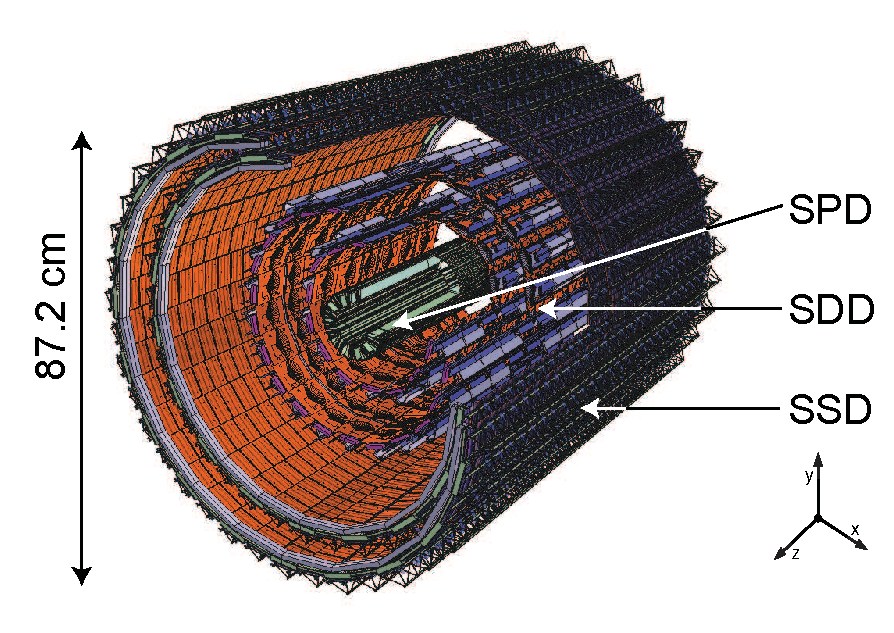
\includegraphics[width=0.75\textwidth]{Figs/Chapter3/its-rf-2-26925.eps}
}
\end{center}
\subfigure[]
{
	\includegraphics[width=0.31\textwidth]{Figs/Chapter3/ALICE-3D-Run1+2-ITS+V0-Inlay-v0-2012-08-02-Highlight-SPD.png}
}
\subfigure[]
{
	\includegraphics[width=0.31\textwidth]{Figs/Chapter3/ALICE-3D-Run1+2-ITS+V0-Inlay-v0-2012-08-02-Highlight-SDD.png}
}
\subfigure[]
{
	\includegraphics[width=0.31\textwidth]{Figs/Chapter3/ALICE-3D-Run1+2-ITS+V0-Inlay-v0-2012-08-02-Highlight-SSD.png}
}
	\caption{Visualisation of the complete structure of the ITS detector (a), as well as a highlight on the SPD(b), SDD(c) and SSD(d) locations in the ALICE apparatus. Figures taken from \cite{alicecollaborationAlignmentALICEInner2017}\cite{maireALICESubdetectorsHighlighted2017}.}
	\label{fig:ITSstructure}
\end{figure}

\begin{table}[t]
    \centering
    \begin{tabular}{b{1.5cm}@{\hspace{0.5cm}} b{1.5cm}@{\hspace{0.25cm}} b{1.5cm}@{\hspace{0.5cm}} b{2cm}@{\hspace{0.5cm}} b{2cm}@{\hspace{0.5cm}} b{1.5cm}@{\hspace{1cm}} b{2cm}@{\hspace{0.cm}}}
    \noalign{\smallskip}\hline\noalign{\smallskip}
	Layer & $r$ (\cm) & $\pm z$ (\cm) & Area ($\m^{2}$) & Active area per module ($\mm^{2}$) & Resolution $r\varphi \times z$ ($\mum^{2}$) & Material budget (\%\Xzero) \\
    \noalign{\smallskip}\hline \noalign{\smallskip}
    1 - SPD & 3.9 & 14.1 & 0.07 & 12.8 $\times$ 69.6 & 12 $\times$ 100 & 1.14 \\
    2 - SPD & 7.6 & 14.1 & 0.14 & 12.8 $\times$ 69.6 & 12 $\times$ 100 & 1.14 \\
    3 - SDD & 15.0 & 22.2 & 0.42 & 72.5 $\times$ 75.3 & 35 $\times$ 25 & 1.13 \\
    4 - SDD & 23.9 & 29.7 & 0.89 & 72.5 $\times$ 75.3 & 35 $\times$ 25 & 1.26 \\
    5 - SSD & 38.0 & 43.1 & 2.20 & 73 $\times$ 40 & 20 $\times$ 820 & 0.83 \\
    6 - SSD & 43.0 & 48.9 & 2.80 & 73 $\times$ 40 & 20 $\times$ 820 & 0.86 \\
    \noalign{\smallskip}\hline\noalign{\smallskip}
    \end{tabular}
    \caption{Details on the six layers of the ITS during the LHC Run-1 and Run-2. \cite{alicecollaborationALICEExperimentCERN2008}\cite{carminatiALICEPhysicsPerformance2004}. The radial distance $r$ are, in fact, average positions. The rightmost column only includes the material budget of the sensor.}\label{tab:ITSspec}
\end{table}

The two innermost layers are positionned at 3.9 and 7.6 \cm from the origin, covering a pseudo-rapidity range of $|\eta| < 2$ and $|\eta| < 1.4$ respectively. At this distance, the track density can reach values up to 80 tracks/$\cm^{2}$. In order to cope with these high track densities, the layers are equipped with SPD employing hybrid\footnote{The term \textit{hybrid} here refers to a type of pixel technology in which the silicon sensor and the readout chip are processed separatedly and connected together via a bump-bonding process. In this way, the detector (silicon sensor) and the electronics (readout chip) can be optimized individually. In LHC experiments, the optimisation is performed such that the detector has a good radiation tolerance and the readout is fast. In return, the assembly tends to be more complex and expensive, the readout chips dissipate a lot of power requiring an efficient cooling system and so more material budget.} silicon pixels. It consists of a bi-dimensional matrix of 256 $\times$ 160 cells of dimension 50 \mum ($r\varphi$) by 425 \mum ($z$). Two matrices are mounted together along the $z$ direction, forming a 141.6 \mm long half-stave. Two of them are attached head to head along the beam direction on a carbon-fibre support with cooling tubes in order to forge a stave. The latter are arranged in ten sectors surrounding the beam pipe, each sector supporting two staves for the inner layer and four for the outer layer. While the high granularity of the SPD provides a spatial resolution of 12 \mum in $r\varphi$ and 100 \mum along $z$, its fast integration time of 100 \nsec -- corresponding to four consecutive bunch-crossings in pp collisions or one in heavy-ions operation -- offers additionnal trigger information.

The SDDs equip the two intermediate layers at an average distance of 15.0 and 23.9 \cm, where the track density rises up to 7 tracks/$\cm^{2}$. Both layers have a pseudo-rapidity acceptance of $|\eta| < 0.9$. The basic module consists in a sensitive area of 70.17 $\times$ 75.26 $\mm^{2}$, split into two drift regions by a central cathode strip at high voltage such that the drift velocity is 8.1 $\mum/\nsec$. At this speed, charges drift to one of the 256 collection anodes (with a 294 \mum pitch) in a maximum time of 4.3 \musec, making it the slowest ITS detector. The SSD modules are mounted on triangular support structure made of carbon-fibre called ladders. The third layer counts 14 ladders with six modules each, and 22 ladders with eight detectors each for the fourth layer. They yield to a spatial precision of 35 \mum in the transverse plane and 25 \mum along the beam axis. 

The two outermost layers are constituted of double sided SSD of 73 $\times$ 40 $\mm^{2}$, where each side has 768 parallel strips (with a pitch of 95 \mum) and corresponds to a side of a p-n junction. The p-side (n-side) of the fifth layer (sixth layer) faces the inside of the ITS. The strips from one side are rotated by a stereo angle of 35 mrad with respect to the other, to reduce the overlapping between the strips and thus the number of ambiguities. The SSD modules are assembled on the same ladder design as those of the intermediate layers: 34 ladders, supporting 22 modules each, are installed on average at 38 \cm from the beam pipe for the inner layer and 38 ladders, holding 25 modules each, at 43 \cm for the outer layer. Both covers a pseudo-rapidity region of $|\eta| < 0.9$. The SSDs layers provide a spatial resolution of the track position of 20 \mum in the $r\varphi$ direction and 820 \mum along $z$, which is essential for the track matching from the Time Projection Chamber to the ITS. Similarly to the SDD layers, its analogue readout allows for the measurement of the charge deposited by the passage of a charged particle, and hence opens the door for PID of low-momentum particles.

Because of the sensitivity of the SDD layers to temperature changes, two thermal shields surround them in order to avoid any radiation of heat.


\subsubsection{Time Projection Chamber}
\label{subsubsec:TPC}

\begin{figure}[t]
\subfigure[]
{
	\includegraphics[width=0.62\textwidth]{Figs/Chapter3/1-s2.0-S0168900210008910-gr2_lrg.jpg}
	\label{fig:TPCFieldCage}
}
\subfigure[]
{
	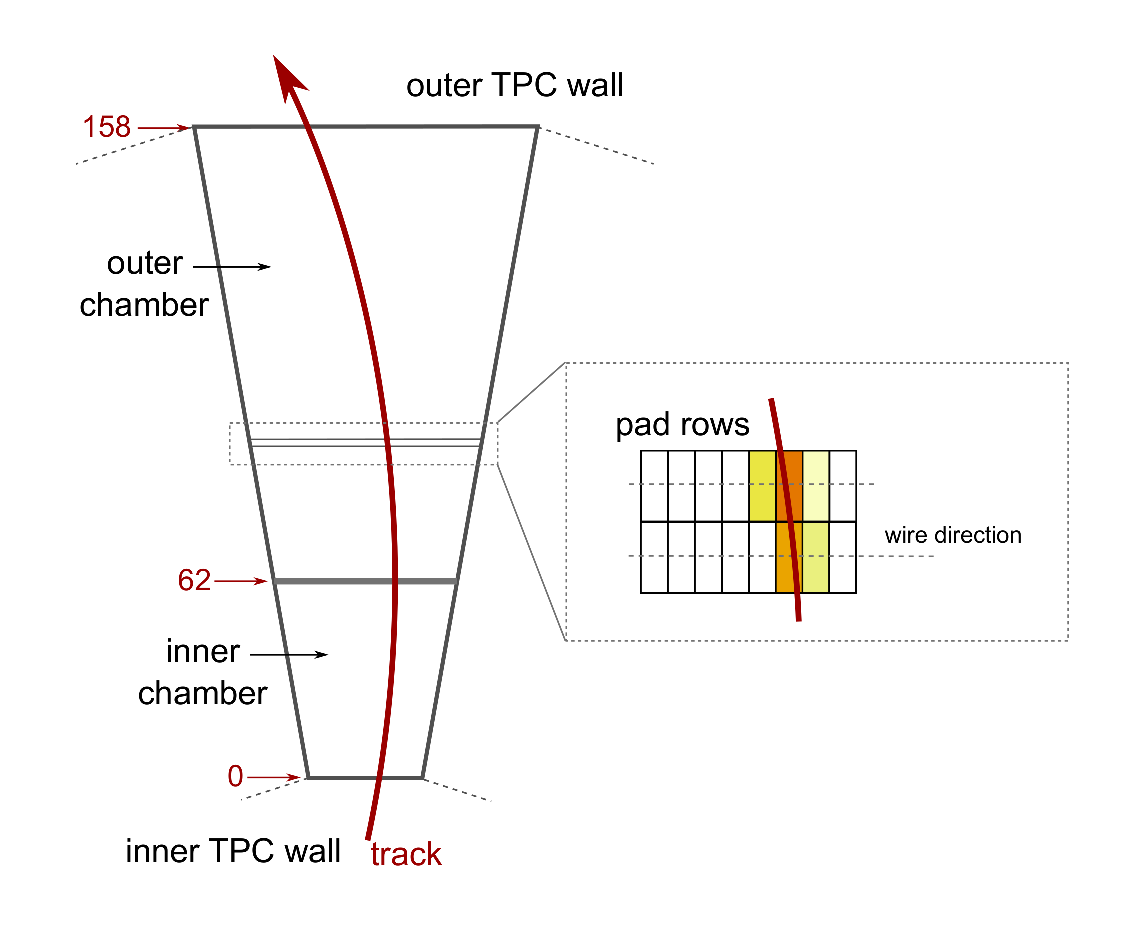
\includegraphics[width=0.50\textwidth]{Figs/Chapter3/Schema-TPC-SecteurEtPadRow.eps}
	\label{fig:TPCSector}
}
	\caption{(Left panel) Scheme of the TPC field cage, taken from \cite{almeALICETPCLarge2010}. (Right panel) Passage of a charged particle through a sector of the TPC. Figure taken from \cite{maireALICETPCSectors2011}.}
	\label{fig:TPCDetector}
\end{figure}

The Time Projection Chamber (TPC) is main tracking device of the ALICE experiment. It is responsible for measuring the momentum of charged particle above 150 \mmom, as well as providing particle identification and vertex determination. The TPC design is shown in \fig\ref{fig:TPCFieldCage}. It consists in a cylindrical gaseous detector, encercling the ITS, with an inner radius of about 85 \cm, an outer radius of 250 \cm and an overall length of 500 \cm along the beam axis. The acceptance of the TPC covers pseudo-rapidities from $|\eta| < 0.9$ (for tracks traversing radially the entire ALICE detector) up to $|\eta| = 1.5$ and the full azimuth (except for the dead zones between sectors). Although this detector occupies a large volume, its material budget remains low (about 3.5\% \Xzero).

The detection volume corresponds to a field cage filled with gas and separated in two equal parts, along the beam axis, by a central electrode at -100 kV. At this high voltage, this central membrane generates an axial electrostatic field of 400 V/\cm. When a charged particle traverses the 88 $\m^{3}$ active volume, it creates electron-hole pairs along its path by ionisation of the gas. The electrostatic field forces the electrons to drift from the central electrode to the end plates, where they are collected, in a maximum time of 92 \musec at a speed of 2.7 \cm/\musec (depending on the gas composition).

Each end plate is segmented into 18 trapezoidal sectors (as represented in \fig\ref{fig:TPCSector}), being themselves instrumented with two multi-wire proportionnal chambers (MWPC) with cathode pad readout: one stretches from $R= 84.8$ \cm to 132 \cm (inner chamber), the other ranges from 134.6 \cm to 246.6 \cm (outer chamber). This is motivated by the variation of the track density with the radius, that requires MWPCs with different wire geometry and pad sizes (granularities). Together, the two chambers count a total of 159 readout pad rows: 63 of 4 $\times$ 7.5 $\mm^{2}$ for the inner chamber, 64 of 6 $\times$ 10 $\mm^{2}$ and 32 of 6 $\times$ 15 $\mm^{2}$ for the outer chamber. They measure the deposited charge, as well as the radial position and the drift time. The longitudinal coordinate is inferred from the latter, provided that the drift speed is uniform over the whole volume\footnote{The longitudinal position is thus given by the product of the drift velocity and the drift time.}. In fact, the gas composition has been optimised for high and stable drift velocity, as well as low diffusion and small radiation length. At the start of the LHC Run-2, a mixture of Ne/CO$_{2}$/N$_{2}$ (90/10/5\%) was employed until 2017. It was later changed for Ar/CO$_{2}$ (90/10\%) as the latter reduces the space-charge distortion [ref?].

\begin{figure}[t]
	\centering
	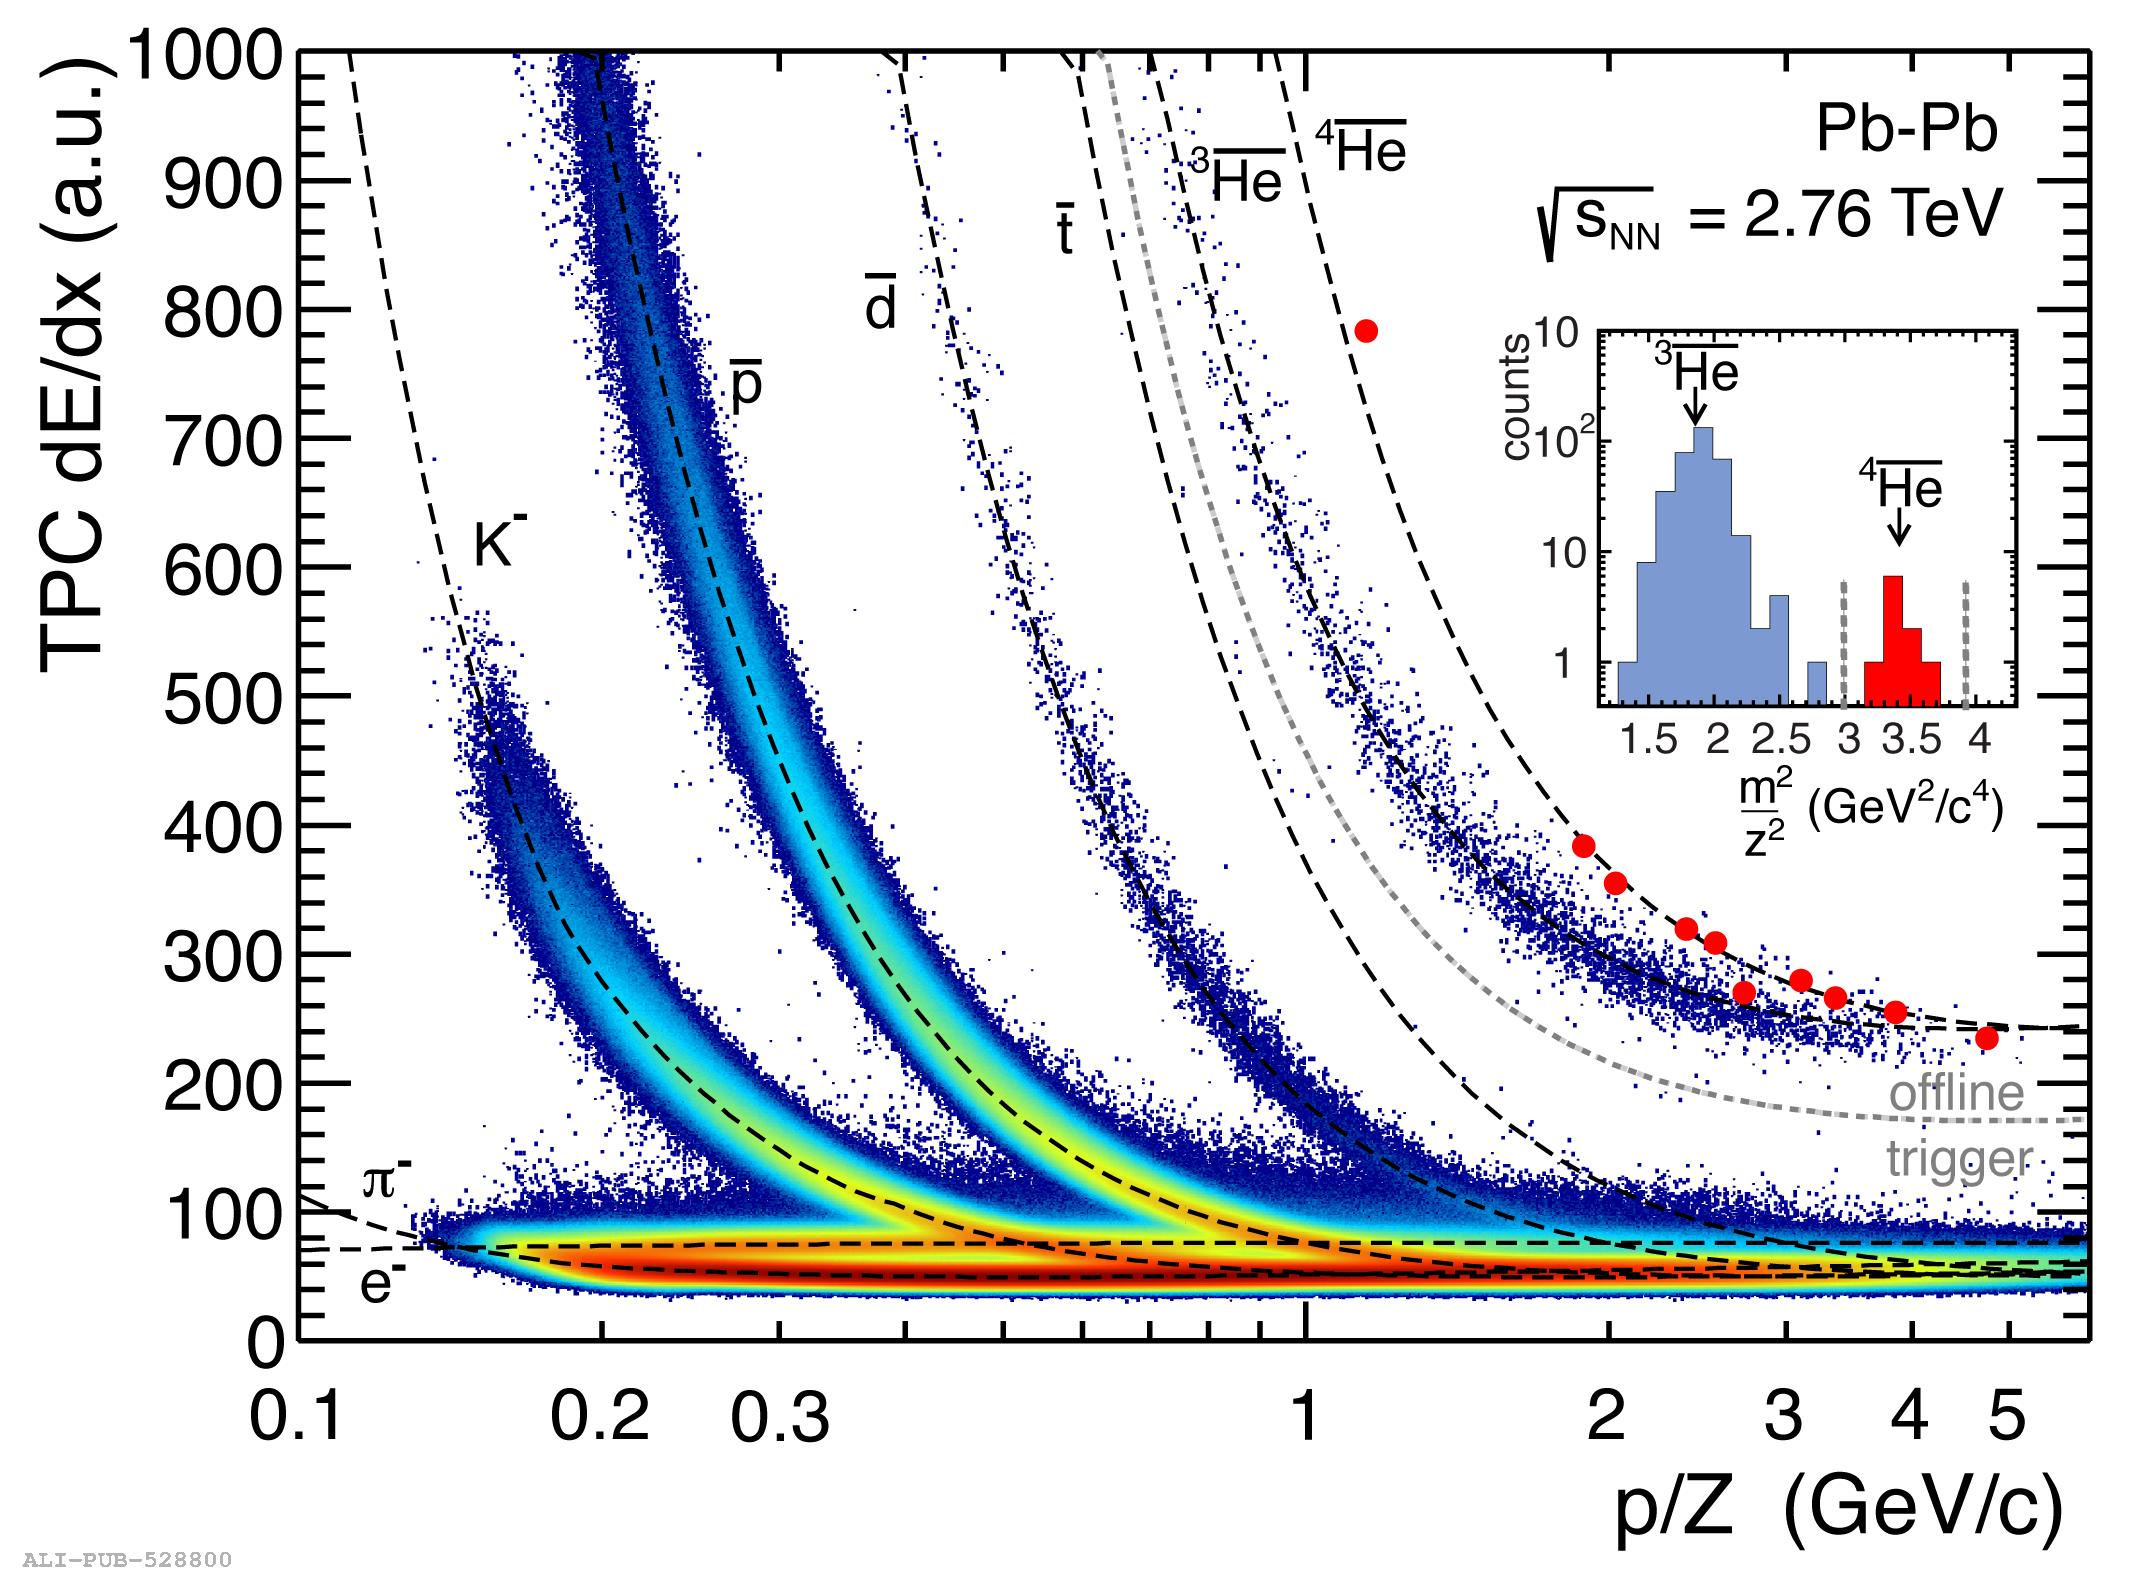
\includegraphics[width=0.8\textwidth]{Figs/Chapter3/dEdx_PbPb_2011_withAlphaInlet_NoLogo.eps}
	\caption{Energy deposition of various charged particles (electron, pion, kaon, anti-proton, anti-deuteron, anti-tritium, and two anti-helium isotopes) in the ALICE TPC in arbitrary units as a function of the magnetic rigidity (momentum over charge number). The dashed lines correspond to the theoretical expectations for each particle species. Figure taken from \cite{alicecollaborationALICEExperimentJourney2022}.}
	\label{fig:TPCdEdx}
\end{figure}

The spatial resolution varies from 1100 to 800 \mum in the transverse plane, and 1250 to 1100 \mum along the beam axis. Although the TPC can not compete with the level of precision of the ITS, it stands as the main tracking detector in ALICE thanks to its almost continuous sampling of the particle trajectory over large distances.

Moreover, the pad rows provides an analogue readout of the charge deposition, that is used to measure the energy loss of charged particles per unit of length (\dEdx) with a resolution ($\sigma_{\rm TPC}$) ranging from 5.5\% in pp events to 6.5\% in the most central Pb-Pb collisions. As the energy deposition is stochastic phenomenon, only the moments of its underlying distribution can be predicted. For instance, the Bethe-Bloch formula describes the mean \dEdx:
\begin{equation}
\begin{split}
\langle -\frac{dE}{dx} \rangle &= K z^{2} \frac{Z}{A} \frac{1}{\beta^{2}} \left[ \frac{1}{2} \ln \frac{2 m_{e} c^{2} \beta^{2} \gamma^{2} T_{\rm max}}{I} - \beta^{2} - \frac{\delta \left( \beta \gamma \right)}{2} \right],\\
\beta \gamma &= \frac{p}{M c}
\end{split}
\label{eq:BetheBloch}
\end{equation}
with 
\begin{itemize}
\item[$\bullet$] $Z$, the atomic number of the absorber (the TPC gas in this case),
\item[$\bullet$] $A$, the atomic mass of the absorber (g.mol$^{-1}$),
\item[$\bullet$] $m_{e}$, the electron mass,
\item[$\bullet$] $z$, charge number of the incident ionising particle,
\item[$\bullet$] $M$, mass of the incident ionising particle,
\item[$\bullet$] $p$, momentum of the incident ionising particle,
\item[$\bullet$] $\beta$, velocity of the incident ionising particle in units of $c$,
\item[$\bullet$] $\gamma$, Lorentz factor of the incident ionising particle,
\item[$\bullet$] $I$, mean excitation energy of the absorber,
\item[$\bullet$] $\delta \left( \beta \gamma \right)$, density effect correction due to the polarisation of the absorber,
\item[$\bullet$] $T_{\rm max} = \frac{2 m_{e} c^{2} \beta^{2} \gamma^{2}}{1 + 2 \gamma m_{e}/M + \left( m_{e}/M \right)^{2} }$, the maximum energy transfer to an electron in a single collision, 
\item[$\bullet$] $K$, a constant.
\end{itemize}

As a matter of fact, the energy deposition follows a Landau distribution. Its broad tail on the high-energy-loss side leads the mean energy loss to be considerably greater than the most probable value. It turns out that the most probable energy loss is much easier to evaluate than the mean, requiring large samples to converge. Thereby, the Landau distribution is usually truncated only to keep the 50 to 70\% smallest values, and by so doing, the truncated mean coincides with the most probable energy loss \cite{particledatagroupReviewParticlePhysics2022}.\\


\Fig\ref{fig:TPCdEdx} shows clearly the characteristic \dEdx bands associated to \electron, \rmPi, \proton, \rmDeuton, \rmTriton, \rmHeThree and \rmHeFour. The measurements distribute around dashed lines, that correspond to the expected mean value given by the Bethe-Bloch formula (\eq\ref{eq:BetheBloch}). By comparing the measured value to the expected energy loss for various particle species, the nature of the incident particle can be determined. The PID estimator
\begin{equation}
n_{\sigma} = \frac{ \langle \dEdx \rangle_{\rm meas} - \langle \dEdx \rangle_{\rm exp, i}}{\sigma_{\rm TPC}}
\end{equation}
gives the distance between measured \dEdx and the expected one under the particle mass hypothesis $m_{\rm i}$ (i $=$ \electron, \rmPi, \proton, \rmDeuton, \rmTriton, \rmHeThree, \rmHeFour), in units of relative resolution $\sigma_{\rm TPC}$. So, the TPC can distinguish a pion/electron from a kaon with a separation power better than 3$\sigma$ below $\sim$ 300 \mmom, and a kaon from a proton up to 1 \gmom.

\begin{figure}[b]
\centering
\subfigure[]
{
	\includegraphics[width=0.6\textwidth]{Figs/Chapter3/ALICE-3D-Run1+2-ITS+V0-Inlay-v0-2012-08-02-Highlight-VZERO.png}
	\label{fig:VZEROinALICE}
}	
\subfigure[]
{
	\includegraphics[width=0.8\textwidth]{Figs/Chapter3/Fig1-4206.png}
	\label{fig:VZEROarrays}
}
	\caption{(Top panel) View of the VZERO scintillator arrays inside the ALICE apparatus: VZERO-A on the left, and VZERO-C on the right. (Bottom panel) Sketches of the VZERO-A (left) and VZERO-C (right) with their segmentation. The dashed lines delimit segments connected to the same photomultiplier tube. Figures taken from \cite{alicecollaborationALICEExperimentJourney2022}\cite{alicecollaborationPerformanceALICEVZERO2013}.}
	\label{fig:VZEROdetector}
\end{figure}


\subsubsection{VZERO}
\label{subsubsec:VZERO}

The VZERO system consists in two scintillator arrays, VZERO-A and VZERO-C, covering the pseudo-rapidity ranges $2.8 < \eta < 5.1$ and $-3.7 < \eta < -1.7$ respectively (\fig\ref{fig:VZEROinALICE}). It plays a crucial role in the data taking of ALICE as it provides minimum-bias triggers for the experiment, measures the charged particle multiplicity and centrality, and participates in the beam luminosity determination.


Each of array is segmented in four rings, themselves being divided in eight sections of 45 wide made of plastic scintillators, as sketched in the \fig\ref{fig:VZEROarrays}. Because of the integration constraints (mainly coming from the muon absorber), two arrays needed to be designed. The 2.5 \cm thick VZERO-A sits at 329 \cm from the nominal vertex ($z = 0$). Since the VZERO-C stands in front of the muon absorber, the scintillator thickness reduces to 2 \cm and its rings are positionned between -86 and -88 \cm along the beam axis. 

\begin{figure}[h]
	\centering
	\includegraphics[width=0.8\textwidth]{Figs/Chapter3/Fig6_2-4228.png}
	\caption{Time of flight of the particles detected in the VZERO-C versus VZERO-A. Figure taken from \cite{alicecollaborationPerformanceALICEVZERO2013}.}
	\label{fig:VZERObeamgas}
\end{figure}

The passage of a charged particle in the scintillator generates light, that is guided to photomultiplier tubes via 1 \mm in diameter Wave-Length Shifting and optical fibers. For each of the 32 elementary cells, the photomultiplier tube outputs two analogue signals. The first measures the integrated charge, the second -- amplified by a factor 10 -- determines the pulse/arrival time relative to the LHC bunch clock with a resolution better than 1 \nsec. Each signal gives rise to a specific type of trigger algorithm. 

Based on the coincidence between the time signals from the arrays, beam-induced background events\footnote{They typically correspond to beam-gas collisions, that is a collision between a bunch from the beam and a residual atom in the beam pipe} can be rejected. \Fig\ref{fig:VZERObeamgas} shows an example of such rejection. A particle coming from the interaction point takes about 11 \nsec and 3 \nsec to reach the VZERO-A and the VZERO-C respectively. If the time of flight of the particles detected in the two scintillator arrays matches these values --- as it is the case in the top right corner of \fig\ref{fig:VZERObeamgas} ---, this would indicate that a beam-beam collision occured. However, the signals arriving in coincidence at -12 \nsec (VZERO-A) and 3 \nsec (VZERO-C), and 11 \nsec (VZERO-A) and -3 \nsec (VZERO-C) are not the signatures of a beam-beam event. They correspond to beam-gas collisions coming from the A-side and C-side respectively. This is the first type of trigger algorithm.

The energy deposited in the scintillators provides a measurement of the charged particle multiplicity. Based on a simulation of VZERO detectors, the total charge collected can be related to the number of primary charged particles. \Fig\ref{fig:VZEROcentrality} shows the relation between these two quantities. The second type of trigger algorithm consists in dividing the distribution of the V0 amplitudes in different multiplicity/centrality\footnote{In heavy-ion collisions, as in \fig\ref{fig:VZEROcentrality}, the impact parameter -- and, \textit{a fortiori}, its percentage value, the centrality -- can not be measured directly. However, since the centrality and the charged particle multiplicity in the event are correlated (confirmed by Glauber fit, that gives access to the centrality), the different intervals in multiplicity are refered as \textit{centrality classes}.} classes from the 5\%-highest multiplicity to the 10\%-lowest multiplicity events, as represented in shaded areas. 

\begin{figure}[h]
	\centering
	\includegraphics[width=0.8\textwidth]{Figs/Chapter3/Fig8-4236.png}
	\caption{Total yield as a function of the signal amplitudes of the two VZERO arrays in Pb-Pb collisions at \sqrtSnn = 2.76 \tev, fitted with a Glauber model in red. The shaded areas correspond to different centrality classes. Figure taken from \cite{alicecollaborationPerformanceALICEVZERO2013}.}
	\label{fig:VZEROcentrality}
\end{figure}

\subsubsection{Time-Of-Flight detector}
\label{subsubsec:TOF}

The Time-Of-Flight (TOF) detector is a large cylindrical array with an inner radius of 370 \cm and an outer one of 399 \cm. It covers the central pseudo-rapidity region, that is $|\eta| < 0.9$, and the full azimuth. While the separation power of TPC only goes up to 1 \gmom, the TOF detector aims at providing particle identification at intermediate momentum from 0.2 to 2.5 \gmom.  To instrument this large volume (17.5 $\m^{3}$), a gaseous detector is employed, as its manufacture remains rather simple and thus inexpensive. The best solution, with respect to the design considerations of the experiment, is the Multi-gap Resistive-Plate Chamber (MRPC) \cite{akindinovMultigapResistivePlate2000}. 

The basic constituent of the TOF system is a pair of MRPC strips, 122 \cm in length and 12 \cm in width, stacked together with an active area of 120 $\times$ 7.4 $\cm^{2}$. As shown in \fig\ref{fig:TOFMRPC}, it consists in two cathodes and a central anode placed in a gas volume and spaced by five 0.4 \mm thin glass plates (with a 250 \mum gap) for each strip. The full volume is filled with a gas mixture composed of C$_{2}$H$_{2}$F$_{4}$(90\%), C$_{4}$H$_{10}$(5\%), SF$_{6}$(5\%), as it shows no ageing effects and  has a rate capability much higher than the expected one in ALICE \cite{akindinovStudyGasMixtures2004}.

\begin{figure}[t]
\hspace*{-1.5cm}
\subfigure[]
{
	\includegraphics[width=0.5\textwidth]{Figs/Chapter3/TOFMRPC.png}
	\label{fig:TOFMRPC}
}
\subfigure[]
{
	\includegraphics[width=0.75\textwidth]{Figs/Chapter3/TOFSuperModule.png}
	\label{fig:TOFStructure}
}	
	\caption{(Left panel) Drawing of the cross section of a 10-gap double-stack MRPC. (Right panel) Schematic view of the TOF barrel with one supermodule, consisting of five modules. Figure taken from \cite{alicecollaborationALICEExperimentCERN2008}.}
	\label{fig:TOFPID}
\end{figure}

To cover the full cylinder along the beam direction and minimise the cumulative dead areas from the innermost to outermost detectors in ALICE, five modules of different lengths are combined. The central element utilizes 117 \cm long module, the intermediate ones 137 \cm, the external ones 177 \cm made of 15 MRPC strips for the central module and 19 for the others. Altogether, they form a supermodule of total length 930 \cm with an overall active region of 741 $\times$ 7.4 $\cm^{2}$, as shown on \fig\ref{fig:TOFStructure}. Each of the 18 azimuthal sectors of the TOF system has a supermodule.

When a charged particle traverses the active volume, it ionises the gas along its path and produces electrons that drift to one of the cathodes. The key aspect of the MRPC resides in the high voltage of the anode (-13 kV), which delivers a high and uniform electrostatic field. The latter is sufficiently strong to start an avalanche process\footnote{Let us consider a medium containing free electrons and in which a strong electrostatic field exists. If the latter is strong enough, it accelerates the electrons such that they will collide with other atoms in the medium, thereby ionising them and releasing additionnal electrons. These ones also get accelerated and collide with other atoms, releasing more electrons, and so on. This chain reaction is called an avalanche process.}, and thereby to give rise to a detectable signal. The avalanche stops when it reaches a glass plate, but the produced electrons continue to drift -- and to create avalanches in the gaseous medium along the way -- until they are collected by the 48 cathode pad readouts of 3.5 $\times$ 2.5 $\cm^{2}$ from each strip. \\

Their output signals carry the information of the deposited charge via the Time-Over-Threshold and the hit time -- with an intrinsic resolution of 56 \psec during the LHC Run-2 -- relative to the collision time, $t_{\rm ev}$. Due to the finite size of the bunches that interact, the latter has to be measured on an event-by-event basis. To that end, different options are available.

The most precise measurement of the collision time is provided by the T0 detector. It consists in two arrays, each made of twelve Cerenkov counters, placed at 375 (T0-A) and -72.7 \cm (T0-C) from the nominal vertex. They respectively cover the pseudo-rapidity range $4.61 < \eta < 4.92 $ and $-3.28 < \eta < -2.97$. Each counter is a quartz radiator of 20 \mm in diameter and 20 \mm thick, connected optically to a PMT. The readout electronics is quite similar to the one used for the TOF detector, with a dead time below 25 \nsec. The T0 system gives two time measurements, $t_{\rm T0-A}$ and $t_{\rm T0-C}$, one for each array. When both values are available, the average is taken as the start time of the event, $t_{\rm ev}^{\rm T0} = \left( t_{\rm T0-A} + t_{\rm T0-C} \right)/2$, with a resolution of 50 and 25 \psec in pp and Pb-Pb collisions. If only one of the two counters produces a signal, the collision time is given by either the $t_{\rm T0-A}$ or $t_{\rm T0-C}$ taking into account the longitudinal position of the primary vertex (provided by the ITS). Consequently, the resolution deteriorates to 100 and 60 \psec in pp collisions for the T0-A and -C respectively, and 50 and 30 \psec in heavy-ion collisions. Due to its limited acceptance, the triggering efficiency of the detector in coincidence is about 48\%, and reaches 60\% and 67\% for the T0-A and -C individually in pp collisions\footnote{The triggering efficiency is close to 100\% in heavy-ion collisions, due to the high multiplicities.}.

The TOF system itself can also determine $t_{\rm ev}$. Based on a sample of particles matching a hit in the detector, a $\chi^{2}$-minimisation procedure is performed in order to extract the set of mass hypotheses that minimises their combined time-of-flights. From this set derives the event collision time, denoted $t_{\rm ev}^{\rm TOF}$. By construction, this procedure only applies for a minimum number of two tracks, and the resolution improves with the track multiplicity (scaling as $\sim 1 / \sqrt{n_{\rm tracks}}$). It allows to reach time resolution from 80 \psec for the low multiplicity events to 20 \psec for the high multiplicity events, with efficiencies ranging from 20\% to 100\% respectively.

Considering the above efficiencies, the collision start time can be obtained from the T0 or TOF measurement ($t_{\rm ev}^{\rm T0}$ or $t_{\rm ev}^{\rm TOF}$) or their combination, if both are available. In the latter case, the final $t_{\rm ev}$ corresponds to their weighted average, with the inverse of their resolution squared as weighting factors. If none of the preceding procedures is usable, the event time is set on the LHC clock\footnote{In fact, it is set on zero as, after alignement and calibration of the TOF detector, the LHC clock phase has been shifted to coincide with the nominal starting time.} which has a resolution of 200 \psec \cite{alicecollaborationDeterminationEventCollision2017}.\\



Hence, the difference between the arrival time $t_{\rm TOF}$ and the moment of the collision $t_{\rm ev}$ gives the \textit{measured time-of-flight} of the charged particle from the primary vertex to the TOF detector. Knowing the latter as well as the the distance travelled, the velocity of the particle -- or rather the ratio of the velocity to the speed of light, $\beta = v /c$ -- can be evaluated. The \fig\ref{fig:TOFPID} shows the distribution of $\beta$ of charged particles measured by the TOF detector as a function of their momentum in Pb-Pb events at \sqrtSnn = 5.02 \tev. A clear separation of the electron, pion, kaon, proton and deuteron bands is visible. This stems from the relation between the particle mass $m$, its momentum $p$ and its velocity $\beta$: 
\begin{align}
m = \frac{p}{\beta \gamma} = p \ \sqrt{ \frac{1}{\beta^{2}} - 1 }& \qquad \textrm{with} \quad \beta = \frac{v}{c} = \frac{L}{c t_{\rm exp}},\\
\Rightarrow t_{\textrm{exp}} &= L \ \frac{\sqrt{p^{2} + m^{2}}}{c p}.
\label{eq:tTOF}
\end{align}

\begin{figure}[t]
	\centering
	\includegraphics[width=0.8\textwidth]{Figs/Chapter3/TOFBetawoMismatchEtaCut_PbPb.eps}
	\caption{Velocity ($\beta = v /c$) of electrons, pions, kaons, protons and deuterons as a function of their momentum (provided by the TPC), measured by the TOF detector, in Pb-Pb collisions at \sqrtSnn = 5.02 \tev. Figure taken from \cite{alicecollaborationALICEExperimentJourney2022}.}
	\label{fig:TOFPID}
\end{figure}

In \eq\ref{eq:tTOF}, $t_{\textrm{exp}}$ corresponds to the \textit{expected time-of-flight}, \ie the time it would take for a particle of mass $m$, with a momentum $p$, to go from the interaction point to the TOF detector following a path of length $L$. To this quantity is attached an uncertainty coming from the track reconstruction, as it will be detailed in \Sec\ref{subsec:EventReco}. By comparing the measured time-of-flight $t_{\rm TOF}$ and the expected one $t_{\rm exp, i}$ for different mass hypothesis $m_{\rm i}$ (i $=$ \electron, \muon, \rmPi, \rmKaon, \proton, \rmDeuton, \rmHeThree, \rmHeFour), particle identification can be performed. The PID estimator $n_{\sigma}$ is constructed in the following way:

\begin{equation}
n_{\sigma} = \frac{t_{\rm TOF} - t_{\rm ev} - t_{\rm exp, i} }{\sigma_{\rm PID, i}}, \qquad \text{with} \quad \sigma_{\rm PID, i}^{2} = \sigma_{t_{\rm TOF}}^{2} + \sigma_{t_{\rm ev}}^{2} + \sigma_{t_{\rm exp, i}}^{2}.
\end{equation}

Therefore, the TOF detector is capable of identifying charged particles in the intermediate momentum range, with a separation power better than 3$\sigma$ between pions and kaons below 2.5 \gmom, and up to 4 \gmom between kaons and protons.

\subsection{Trigger system and data acquisition}

As opposed to its LHC Run-3 version, ALICE only recorded triggered data in the Run-1 and -2, \ie events are selected and stored based on a variety of different features. The Central Trigger Processor (CTP) is in charge of optimising the trigger system in order to make the best use of i) the various detector components, that are busy for different period of time ($\sim$88 \musec for the TPC versus the T0 with $<$25 \nsec) when a valid trigger signal is received, and ii) the different running modes (pp, pPb, PbPb with specific interaction rates).\\

The latter is achieved by ensuring that the data collection is not ruined by the pile-up. Here, we refer primarily to event pile-up between different bunch crossings, that is treated differently depending on the expected multiplicity and luminosity. The one occuring between two central or semi-central heavy-ion collisions must be avoided as the density of tracks is so high that they become unreconstructable. However, the pile-up level between a (semi-)central and up to two peripheral Pb-Pb collisions is tolerable in some detectors -- such as the TPC -- and not in others -- the ITS for example. The same applies for pp collisions where pile-up is unavoidable but tracks are reconstructable due to much lower track densities than in Pb-Pb. To that end, a \textit{past-future} protection has been implemented, which basically verifies that the level of pile-up in the sensitive time windows of each detector\footnote{For instance, the past-future protection circuit checks on the TPC that the pile-up occuring between -88 \musec (past) and +88 \musec (future) relative to the collision time stays managable. The same logic applies to the rest of the ALICE devices. In fact, three categories of detectors can be drawn: the ones that can provide a signal at each bunch crossing and thus do not not need a protection, the others requiring the application of the past-future condition under 10 \musec, and the TPC demanding a protection under 88 \musec.} remains tolerable as defined in the above requirements.\\

To ensure efficient data taking, the ALICE detector is not entirely readout for every event. Instead, it is divided into groups of sub-systems named detector \textit{clusters}. For instance, the data from the forward muon arm do not need the TPC to be exploitable, only the trigger detectors (in particular the V0 and SPD for determining the centrality/multiplicity class and primary vertex location) are required. By grouping these detectors into the same cluster, they can be read out separately from the other devices. Consequently, there are three detector clusters comprising the full detector, only the central detectors, and the forward muon detectors (with the trigger detectors) respectively.

In addition, the hardware trigger system divides into three levels -- dubbed L0, L1 and L2 -- with different latencies \cite{bloodworthALICECentralTrigger2000}\cite{alicecollaborationTriggerDataAcquisition}. At each LHC clock cycle (that is every 25 \nsec in pp and 100 \nsec in heavy-ion mode), the CTP checks for the inputs from detectors with fast trigger capabilities (essentially the T0, V0, SPD and TOF) up to 800 \nsec after the collision (time needed for the SPD to transmit its trigger signal to the CTP). When the inputs coincide with the requirements of one (or more) \textit{trigger class}\footnote{This is the set of detector signals that defines a trigger selection. The ALICE experiment counts 50 trigger classes \cite{alicecollaborationALICEExperimentCERN2008}.}, the trigger system issues a Level 0 (L0) decision in less than 100 \nsec, that reaches the detectors 1.2 \musec after the interaction. Upon reception of the L0 signal, detectors move into a busy-state in which they stop taking new data until they have been fully read out. Since all the detector inputs can not be transmitted under 800 \nsec, the CTP collects all the signals that can be delivered under 6.1 \musec, checks the conditions for all trigger classes and -- in the absence of a veto from the past-future protection circuit -- generates a Level 1 (L1) trigger arriving at the detectors 6.5 \musec after the collision. Together, the L0 and L1 signals represent the fast response of the trigger system. The last signals arrives 87.6 \musec after the collision, due to the drift period of the TPC. A level 2 (L2) trigger decision is sent with a latency of 100 \nsec and reaches the detectors at 88 \musec, to finally conclude on whether the event is accepted or rejected. At this stage, a rejection most often comes from the excessive pile-up.\\

Among the different trigger classes, two configurations play an important role in ALICE and in the present work: the minimum-bias (MB) and the high-multiplicity (HM) classes. As its name suggests, the former refers to the least biasing conditions for the data acquisition in ALICE over the full multiplicity distribution. Its requirements have evolved over the years. Because of the low interaction rate in pp in 2009 and 2010 data takings, the minimum-bias trigger selections were kept loose: it required a hit in either VZERO counters or in one of the two SPD layers (MB$_{\rm OR}$). In this way, the collected event would have at least one charged particle in eight units of pseudo-rapidity. As the luminosity and the amount of beam-gas background increase, the conditions were tightened up and the high selection efficiency MB trigger is traded off for a high purity one. Hence, to be recorded, an event necessitates a coincidence between the VZERO detectors (MB$_{\rm AND}$). This is equivalent of asking for, at least, one charged particle in the A- and C-side, separated by 4.5 units of pseudo-rapidity\footnote{In fact, there exists still a few variants of the minimum-bias trigger such as at least a one hit in the SPD, or one hit in either VZERO scintillator arrays, or even both simultaneously.} \cite{alicecollaborationChargedparticleMultiplicityMeasurement2010}\cite{alicecollaborationALICETriggerCoordination2020}. 

The HM trigger corresponds to 0.1\% highest multiplicity events from the MB sample; it has been implemented in order to study efficiently rare signals, and most particularly in small systems. Throughout the LHC Run-1, it was based the number of hits in the outer layer of the SPD for the multiplicity estimation. The threshold was typically set between 80 to 100 hits which represent about 60 to 80 pairs of matching clusters between the two SPD layers, also refered as SPD tracklets (HM$_{\rm SPD}$) \cite{alicecollaborationALICETriggerCoordination2020}. However, in the Run-2, the default HM trigger configuration changes and the threshold now relies on the signal amplitude of the VZERO counters, that correlates with the event multiplicity (HM$_{\rm VZERO}$). 

As a side note, the trigger system operates in two modes: the default option, called "CENT", corresponds to the one where events are recorded with the informations of the SDD; if this detector is busy at the reception of the L0 signal, the "FAST" configuration allows to record the event without reading out the SSD. Because it is the slowest ITS detector (4.3 \musec) compared to the others (300 \nsec for the SPD and 1.4 to 2.2 \musec for the SSD), the SDD limits significantly the triggering rate. By combining these two trigger configurations (CENT and FAST), one can double the amount of data available but at the price of a lower track reconstruction efficiency (\ref{subsec:TrackReco}).\\

The reception of a successful L2 trigger signal initiates the detectors readout. Each one produces \textit{event fragments} that are transmitted to Data AcQuisition (DAQ) readout receiver cards, being themselves linked to Local Data Concentrators (LDCs). The latter gathers the event fragments from its associated cards and assembles them into sub-events. In parallel, a copy of the readout data is transfered to the High-Level Trigger (HLT) farm computer, that performs an online processing in order to filter out interesting physics events with more sophisticated and precise selections (jet identification, sharp \pT cut, etc) than the lower layer triggers (L0, L1, L2). It can also reduce the output size by selecting relevant parts of the event. The triggered event or the regions of interests are compressed, transfered back to the LDCs. The DAQ system treats the output of HLT system as the one of any other sub-detector.

A single machine of the Global Data Collector (GDC) farm\footnote{The Event-Destination Manager (EDM) supervises the distribution of LDC's sub-events from the same event to single GDC machines, and balances the data stream in order to avoid event loss by overloading the GDC farm (the so-called back-pressure). The latter point is critical for the reconstruction of rare events, as more frequent events take up most of the GDC load. Hence, the EDM monitors their GDC occupancy and, in case it is too high, they are blocked in favour of the rare events. With the past-future protections, these are the causes of a rejection at the L2 trigger stage.} receives the sub-events from sub-detectors' LDCs --- including the ones from the HLT computers -- and proceeds to the event reconstruction. The Transient Data Storage archives the output data over the storage network before their final recording into the Permanent Data Storage.


\subsection{The event reconstruction}
\label{subsec:EventReco}

The event reconstruction starts at the DAQ-LDC level, where the digitised signals of each detector -- likely generated by the same particle -- are grouped into a \textit{cluster}, based on their space and/or time proximities. Its centre of gravity is often taken as an estimate for the crossing point of a particle in the sensitive volume of the detector.

\subsubsection{Preliminary determination of the primary vertex}

From these clusters in the two innermost layers of the ITS, a preliminary estimation of the primary vertex position is realised \cite{caffarridavideCharmSuppressionPbPb2012}. The pairing of SPD clusters between the inner and outer layers (within an azimuthal window of $\Delta \phi = 0.01$ rad) allows to form tiny track segments\footnote{The track curling being supposedly small between the radii of the two SPD layers (3.9 and 7.6 \cm), it can be approximated as a straight line, in particular in the case of high-momentum particles \cite{carminatiALICEPhysicsPerformance2004}.} called \textit{tracklets}. The space point towards which the maximum number of tracklets converges gives a first estimate of the primary vertex location. 

Concretely, the reconstruction algorithm attempts to minimise the quantity
\begin{equation}
D^{2} = \sum_{i}^{N} \left( \frac{x_{i} - x_{0}}{\sigma_{xi}} \right)^{2} + \left( \frac{y_{i} - y_{0}}{\sigma_{yi}} \right)^{2} + \left( \frac{z_{i} - z_{0}}{\sigma_{zi}} \right)^{2},
\label{eq:SPDVertexer}
\end{equation}
with $N$ the number of considered tracklets, and each term of the sum corresponds to weighted distance along $x$, $y$ or $z$ between the tracklet $i$ ($x_{i}, y_{i}, z_{i}$)\footnote{Here, this is the tracklet's position at the point of minimum distance with respect to the primary vertex. At the start of the minimisation procedure, the initial location of the vertex is taken as the mean position of the intersection point of all selected tracklets \cite{carminatiALICEPhysicsPerformance2004}.} and the interaction point ($x_{0}, y_{0}, z_{0}$). The minimisation procedure is repeated several times; at each iteration, the tracklets contributing to a previously found vertex are discarded from the sample. Hence, by construction, the first reconstructed vertex takes up the majority of the contributing tracklets and is designated as the primary one. Since the spatial resolution scales as $1/\sqrt{N_{\rm tracklets}}$, the latter also turns out to be the most accurate. 

In cases where no convergence point is found (as it happens in low-multiplicity events), the algorithm searches for a vertex along the beam axis, with the constraint that it coincides with the beam position in the transverse plane. It is calculated as the weighted mean of the intersection points with the beam axis over all the tracklet candidates.

If no pair of clusters can be formed in the SPD, the primary vertex and thus the event are not reconstructed.

\subsubsection{Track reconstruction}
\label{subsubsec:TrackReco}

The determination of the trajectory --- or \textit{tracking} in the particle physicist's jargon --- of a charged particle breaks down into two major phases: the \textit{track finding} and \textit{track fitting}. The former aims at associating a set of clusters to the same track, and from this, the latter tries to estimate the track parameters such as the charge or momentum. Both can be performed using global or local methods.

Broadly speaking, the global approach treats all the measurements simultaneously, once all the informations have been collected. It has the advantages of being stable with respect to noise and directly applicable on raw data, but it does a require a precise knowledge of the model that may be unknown or do not exist because of random perturbations or non-uniformity of the magnetic field for instance. The online event reconstruction on the HLT computer farm typically uses such techniques (Cluster Finder and Track Follower methods, fast Hough transform), primarily because they are fast but also an extremely high precision is required at this stage (mostly interested in the reconstruction of high-momentum particles).

In contrast, the local methods proceed to a progressive estimation of the parameters  from one measurement to the next, each step improving the knowledge about the trajectory. Thereby, they do not require to know the global model, as any local effect (stochastic processes, etc) can be naturally accounted for at each data point. However, they are also sensitive to the noise, wrong measurement or misassociation, and rely on complex reconstruction algorithms. Among all the local approaches, the most advanced one is the Kalman filter technique, which is the one adopted for the offline reconstruction in ALICE. 

Within the framework of the Kalman filter, the five track parameters at a given time (or equivalently, at the position of a given hit) are contained inside the \textit{system state vector}. The latter evolves according to an iterative procedure in two steps. 
\begin{itemize}
\item[$\bullet$] \textbf{Prediction:} The track parameters are extrapolated to the next detection plane, by the sum of a deterministic term -- depending only on the current knowledge of the state vector -- and a noise term accounting for stochatistic processes such as multiple scattering or energy loss.
\item[$\bullet$] \textbf{Filtering:} If a cluster at the extrapolated position is found in the proximity of the predicted measurement, it is added to the prediction and thus improving/updating the state vector. In this way, cluster association with a track (track finding) appears naturally and simulatenously with the track fitting.
\end{itemize}
These steps repeat as many times as there are measurement points. There also exists a third (optional) phase, called \textbf{smoothing}, available once the full state vector has been extracted: the prediction and filtering steps are replayed in the opposite direction, starting from the last filtered point. These can be reiterated as much as required; each pass refining the track parameters such that the reconstructed track reproduces more and more the real particle trajectory.

Note that the two aforementionned random perturbations of the particle trajectory are in fact treated differently\footnote{This originates from the different stochastic nature of these processes. The multiple scattering follows a Gaussian distribution with a zero mean value and a variance given by the Molière theory \cite{particledatagroupReviewParticlePhysics2022}. In other words, the associated noise term should be unbiased ($\langle \epsilon \rangle = 0 $) with a known covariance matrix. In contrast, the energy loss leads to a biased noise term ($\langle \epsilon \rangle \neq 0 $), given by the Bethe-Bloch formula. However, it should be most notable for small particle energies where multiple scattering dominates, and so, no error term is added to the covariance matrix.}. On one hand, the multiple scattering introduces an angular uncertainty on the position of the next measurement, which translates into an increase of the covariance matrix elements of the state vector. On the other hand, the energy loss affects the momentum of track parameters, but can be estimated on average knowing the amount of crossed material and using the Bethe-Bloch formula in \eq\ref{eq:BetheBloch} under the assumption of a certain particle mass. Hence, a correction of the \dEdx of the track can be applied at each prediction step. \\

In ALICE, the Kalman-filtering track reconstruction uses three passes, as illustrated in \fig\ref{fig:Kalmanfiltering}. 

The first inward stage (first path on \fig\ref{fig:Kalmanfiltering}) starts by looking for the first clusters of a track candidate, dubbed \textit{track seed}, in order to initate the Kalman-filter procedure. This search commences in the best tracking device of the experiment, \ie the TPC, and particularly at its outer radius where the low track density limits the number of ambiguous cluster association. At first, the seeds consist of two TPC clusters and the preliminary vertex point. This initial guess relies on the fact that the track originates from the interaction point. This process is reiterated later without such constraint, which would correspond to secondary tracks coming from a decay. In this case, the seeds are formed out of three clusters.

Once the seeds have been built, they are propagated inwards to the TPC inner radius.
As described above, at each step, the seeds are updated with the nearest space point whenever one passes a proximity cut, taking into account the multiple scatterings and energy losses. At the end, only the tracks with at least 20 (up to 159 possible) attached clusters, and that a minimum of 50\% of the predicted measurement points matches an associated hit, are selected. 

\begin{figure}[!t]
	\centering
	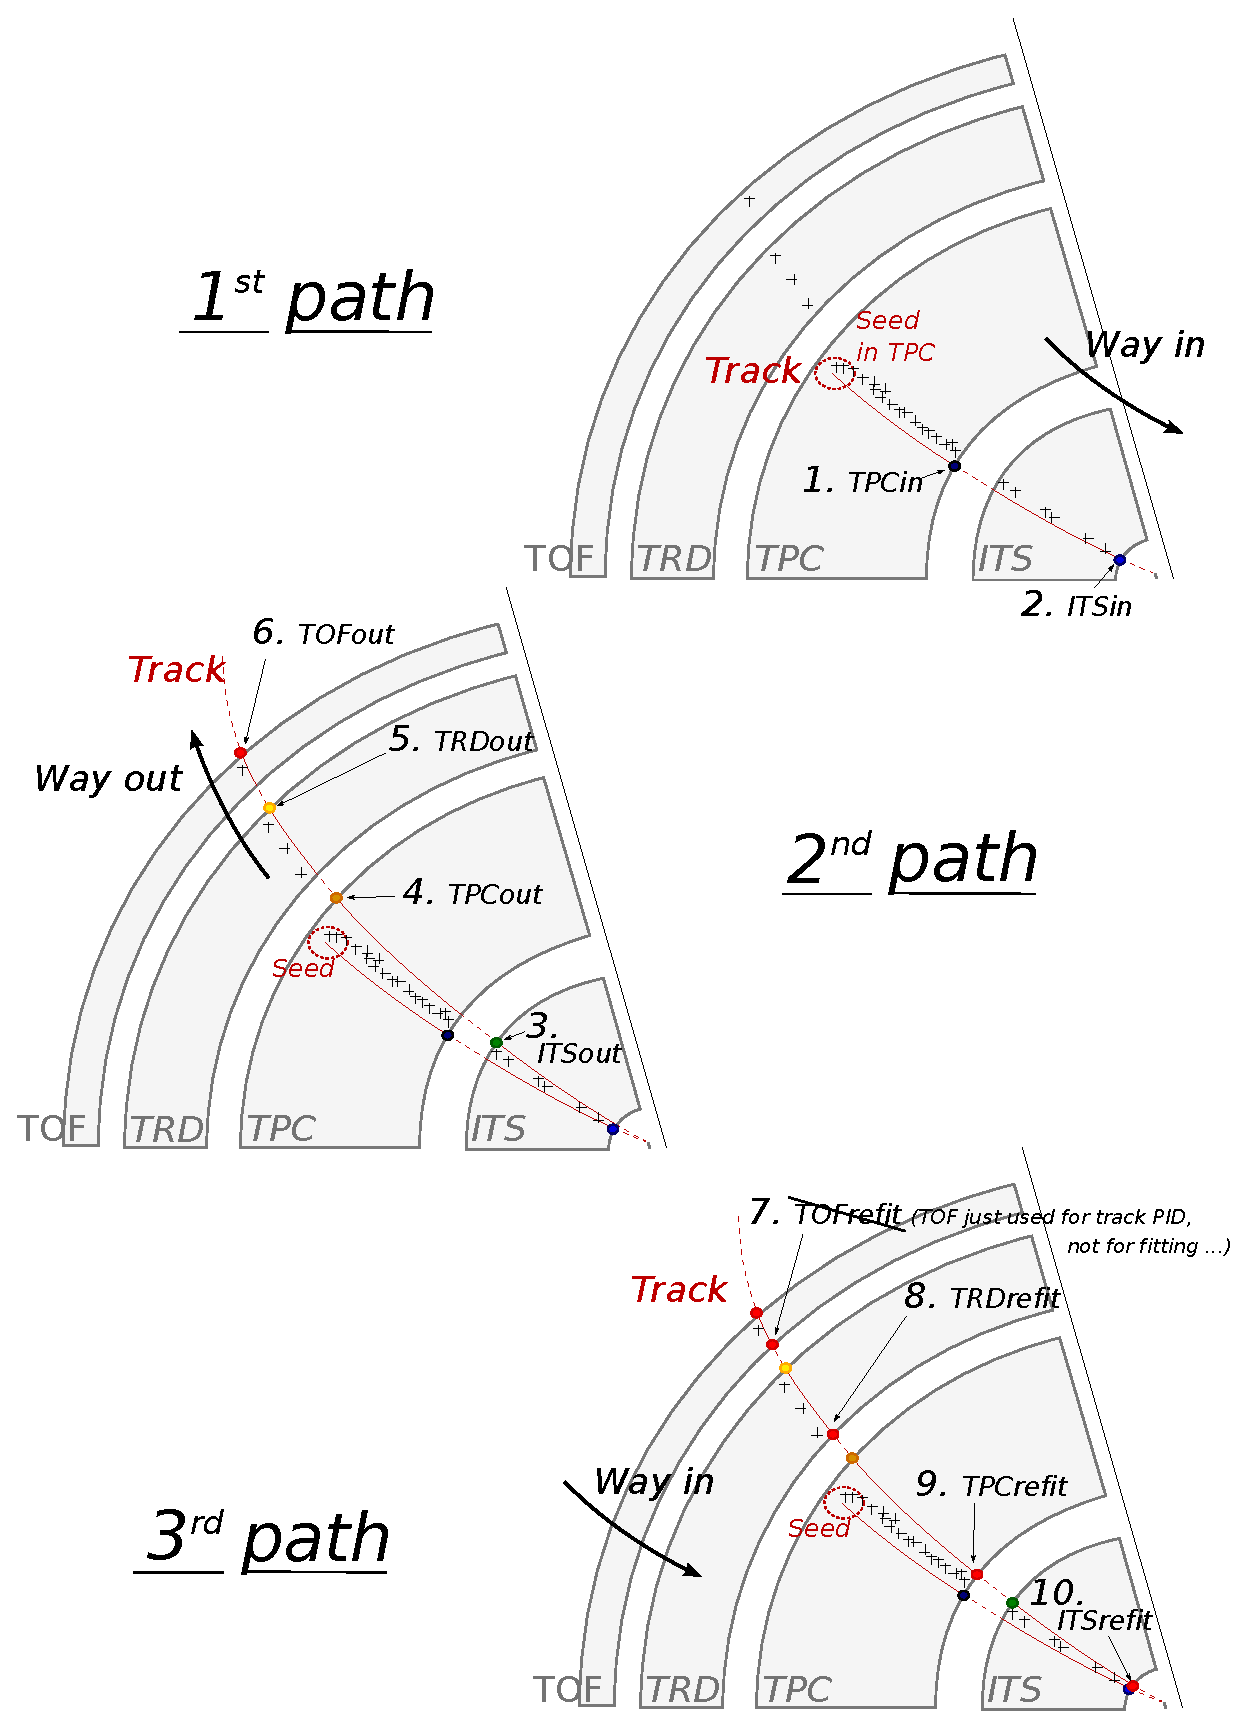
\includegraphics[width=1.05\textwidth]{Figs/Chapter3/Schema-PcpTrackingALICE.eps}
	\caption{Overview of the different elements of the track reconstruction in ALICE, at each pass of the Kalman filter. Figure taken from \cite{maireTrackReconstructionPrinciple2011}.}
	\label{fig:Kalmanfiltering}
\end{figure}

During this propagation, a preliminary particle identification based on the energy deposit in the TPC gas (see \Sec\ref{subsubsec:TPC}) allows to determine the most probable mass of the track candidate among eight hypothesis: \ePlusMinus, \muPlusMinus, \rmPiPlusMinus, \Kplusmin, \pOrPbar, \rmDeutonPM, \rmTritonPM, \rmHeThreePM or \rmHeFourPM. In cases where there is an ambiguity, the pion mass is assigned by default. From this and the amount of crossed material at each step, energy losses can be corrected on average using the Bethe-Bloch formula (\eq\ref{eq:BetheBloch}). It should be emphasised that all the parameters related to the TPC corresponds, in fact, to those of Ne. This approximation is justified by i) the fact that the TPC gas consists mainly of this element (until 2017), and ii) the effect is relatively small. 

When all the seeds have reached the inner wall of the TPC, the tracking in the ITS takes over. The reconstructed TPC tracks are extrapolated from the TPC inner wall ($\sim 85$ \cm) to the outermost layers of the ITS (38 and 43 \cm), that serve as seeds for the track finding in the ITS. Similarly as in the TPC, the seeding procedure produces two kinds of seed: first, one with vertex constraint, then the other without it. Whatever the hypothesis, they are all propagated as close as possible to the primary vertex, and updated along the way by any cluster passing a proximity cut. Only the highest quality candidates in the ITS from each TPC track are selected. A further check on cluster sharing among each other is performed. In such a case, the tracking algorithm tries to find another candidate and if this fails, the worst of the two tracks receives a special flag for containing a shared cluster, that is a potentially incorrectly assigned cluster.

Once all the ITS-TPC tracks have been formed, the ITS standalone tracking procedure comes into play and uses the remaining clusters to recover unfound tracks in the TPC because of i) their very low momentum or ii) the deadzones between sectors, or iii) decays before reaching the chamber. Formed out of two clusters from the three innermost layers and the preliminary vertex point, the seeds are propagated to the other layers, and updated with clusters passing a proximity cut. Only the track hypothesis with the smallest reduced $\chi^{2}$ is kept, and its assigned clusters are removed from further track finding. The procedure repeats until there are no more track to search. 

Upon completion of the track reconstruction in the ITS, the first stage of the tracking ends with the extrapolation of all tracks to their point of closest approach to the preliminary primary vertex. As in the TPC, energy loss corrections are applied at each propagation step in the ITS, considering the same mass hypothesis as one used previously and assuming that all the materials in the ITS volume (including the beam pipe) are made of Si\footnote{This relies on the same reasons as the ones mentionned in the case of the TPC. The \chap\ref{chap:CPTAnalysis} will showcase the limits of this approximation.}.\\

The second stage starts with the outwards propagation from the primary interaction point to the outermost layers of the ITS, and then towards the TPC outer wall (second path on \fig\ref{fig:Kalmanfiltering}). Based on the track parameters from the first iteration, the Kalman filter goes in the outward direction through the previously associated clusters. This also allows to calculate the track length integral, as well as the expected time of flight for the eight particle mass hypothesis, which are updated at each step. When reaching the outer edge of the TPC, the Kalman filter stops updating the track parameters but continues the propagation further detector (TRD, TOF, EMCal, PHOS, HMPID) for to hit matching. The track length integration and time-of-flight calculations terminates upon arriving at the TOF detector. \\

At the final stage (third path on \fig\ref{fig:Kalmanfiltering}), starting from the TPC outer wall, all tracks are propagated inwards to their distance of closest approach (DCA) to the preliminary primary vertex. Along the way, their parameters are improved one last time with the previously associated clusters in each detector. \\

\begin{figure}[t]
	\centering
	\includegraphics[width=0.9\textwidth]{Figs/Chapter3/PTresolution_vs_1Pt_pPb_2013_PerfPaper-8441.png}
	\caption{Transverse momentum resolution for TPC standalone and ITS-TPC combined tracks, with and without vertex constraint, as a function of $1/\pT$ in p-Pb collisions at \sqrtSnn = 5.02 \tev. The blue squares can not be seen as they overlap withe green ones. Figure taken from \cite{alicecollaborationPerformanceALICEExperiment2014}.}
	\label{fig:MomResolution}
\end{figure}

The reconstruction efficiency of TPC standalone tracks saturates around 80-85\% for transverse momentum above 0.5 \gmom, due to the loss of clusters in the deadzones between sectors. At lower \pT, it drops rapidly because of the dominance of multiple scattering and energy loss in the detector material. Whatever the detector occupancy, the contamination of wrongly associated clusters in the TPC remains low; it does not exceed 3\% for tracks with more than 10\% of fake clusters, even in the most violent heavy-ion collisions.

The TPC track prolongation efficiency to the ITS shows little dependence on the transverse momentum. It reaches $\sim$ 95\% for tracks with at least two associated hits in the ITS, and decreases to about 80\% in pp collisions at \sqrtS = 7 \tev (75\% in Pb-Pb collisions at \sqrtSnn = 2.76 \tev) when they have a minimum of one hit over two SPD layers, the furthest detectors relative to the TPC. The contamination of wrongly associated ITS clusters, though, can be quite high: $\sim$ 30\% of tracks with at least one fake cluster below $\pT < 0.2$ \gmom, $\sim$ 7\% at 1 \gmom, and below 2 \% at 10 \gmom in the most central Pb-Pb collisions.

The \fig\ref{fig:MomResolution} shows the resolution on the inverse transverse momentum for TPC standalone and ITS-TPC combined tracks, extracted from their covariance matrix. This quantity is related to the relative transverse momentum resolution, $\sigma_{\pT}/\pT$, via 
\begin{equation}
\sigma_{1/\pT} = \frac{\sigma_{\pT}}{\pT} \frac{1}{\pT} \quad \Rightarrow \quad \frac{\sigma_{1/\pT}}{1/\pT} = \frac{\sigma_{\pT}}{\pT}.
\end{equation}
In general, the transverse momentum resolution varies as a function of the transverse momentum; typically, it is at least as good as 0.9\% at $\pT = 1$ \gmom and 6\% at $\pT = 10$ \gmom. Note that the global ITS-TPC tracks always yields to a better relative \pT resolution than those reconstructed only with the TPC. In the latter case, the vertex constraint on the seeding strongly improves the resolution but the effect is negligible with a matching to the ITS detectors.


\subsubsection{Final determination of the primary vertex}

The end of tracking stage initiates a new determination of the primary vertex, based on the ITS-TPC combined tracks. Unlike the tracklets, their curvature is known, which allows to find the interaction point with a much higher precision.\\

All the global tracks are extrapolated as close as possible to the nominal beam position (or luminous region\footnote{When two beams collide, it gives rise to one or multiple collisions. Their interaction point \textit{a priori} lies anywhere within the region defined by the convolution of the particle distribution -- in other words, the beam size -- of the two incoming beams. Also called \textit{interaction region}, its transverse size is given by $\sigma_{D} = \sigma^{\rm beam} / \sqrt{2}$ \cite{carminatiALICEPhysicsPerformance2004}.}). After rejection of far outliers, the approximate point of closest approach of all selected tracks provides a first estimation of the interaction vertex. From here, in the near vicinity of its true position, a highly precise vertex fit can be performed \cite{karimakiEffectiveVertexFitting1997}. It basically consists in finding the space point that minimises the weighted\footnote{The track weighting has the effect of suppressing the contribution of any remaining outliers.} distance of closest of approach to this same point over all the tracks, as in \eq\ref{eq:SPDVertexer}. 

The precision on the vertex position increases with the number of tracks employed in the fitting algorithm. Therefore, in low-multiplicity events, the fit also includes the nominal beam position as an additional constraint/contribution with an uncertainty corresponding to the transverse size of the luminous region \cite{karimakiEffectiveVertexFitting1997}. Although high-multiplicity events have plenty of tracks available, the high pile-up rate requires a different approach. In order to reduce the contamination from collisions, only tracks coming from the same bunch crossings (identified thanks to the time information measured in the TOF detectors) can contribute to the same vertex. To further suppress the contribution of outliers, the vertex fitting relies on a more robust technique based on Tukey bisquare weights \cite{alicecollaborationPerformanceALICEExperiment2014}. \\

The \fig\ref{fig:VertexResol} shows the transverse resolution on the primary vertex position as a function of the particle multiplicity per unit pseudo-rapidity in pp at \sqrtS = 7 \tev. As mentioned above, the accuracy on the interaction point position sharply improves with the track multiplicity in the event, reaching $\sim 50$ \mum for $\dNdeta > 15$. With respect to the preliminary vertices found with the SPD tracklets, the final ones determined with global tracks is better by at least a factor of two. Note that both resolutions scale as the square root of the number of contributing tracks/tracklets \cite{caffarridavideCharmSuppressionPbPb2012}.

\begin{figure}[t]
	\centering
	\includegraphics[width=0.9\textwidth]{Figs/Chapter3/VertexRes-8462.png}
	\caption{Transverse width of the final vertex distribution, in solid markers, in pp collisions at \sqrtS = 7 \tev. Two contributions are separated: the transverse size of the nominal beam position $\sigma_{\rm D}$, and the transverse resolution on the vertex $\alpha / \sqrt{ \left( \dNdeta \right)^{\beta} }$. For comparison, the open markers show the same quantity determined making use of SPD tracklets. Figure taken from \cite{alicecollaborationPerformanceALICEExperiment2014}.}
	\label{fig:VertexResol}
\end{figure}

\subsection{The ALICE offline framework}

\subsubsection{The computing model}

Over the whole LHC Run-2, more than 160 PB of raw data have been collected by the ALICE experiment. Their treatment requires a robust framework, capable of processing them in a reliable and timely fashion. 

To be processed, this volume of data requires an amount of computing resources that can not be concentrated in one place\footnote{There are various reasons. Although the funding agencies invest in the computing equipment of their scientific projects, they focus their investments in their own countries. Even if all computing resources could be put in one place -- let us say, at CERN --, the manpower would be insufficient to ensure the upkeep of such a system.}. Instead, it is spread over different computing centres around the world. In particular, ALICE uses the Worlwide LHC Computing Grid (WLCG), a worldwide computer network infrastructure coordinated by the CERN and shared among all LHC experiments, that includes over 170 computing centres in 42 countries. The WLCG stands as the world's largest computing grid, that provides near real-time access to the LHC data regardless of their physical location \cite{worldwidelhccomputinggridWorldwideLHCComputing}.

\begin{figure}[b]
	\centering
	\includegraphics[width=0.8\textwidth]{Figs/Chapter3/WLCG-Tiers-2021_v3_1.png}
	\caption{The three Tiers of the Worlwide LHC Computing Grid as of 2023, with the list of the thirteen Tier-1 computing centres, with their geographic location. Figure taken from \cite{worldwidelhccomputinggridWorldwideLHCComputing}.}
	\label{fig:WLCG}
\end{figure}

The WLCG computing sites follows a hierarchical structure in layers or \textit{Tiers} as shown in \fig\ref{fig:WLCG}, that provides different levels of data storage and processing. The Tier-0 corresponds to the CERN Data Centre located in Geneva, that directly receives all the raw data from the LHC experiments, keeps one replica (on magnetic tapes) and performs the first reconstruction pass. It also distributes the raw data and the reconstruction output to the thirteen Tier-1 computer centres around the world via high-speed connections between 10 and 100 GB/\second. They share the same roles with CERN, namely safe-keeping the data, finishing their reconstruction and distributing them to the next layer. The Tier-2 regroups about 160 sites, corresponding typically to universities and scientific institutes, that store the data produced by the closest Tier-1 site. Beyond their mass-storage capabilities, they are used to run the physics analysis tasks, produce Monte Carlo simulations, and reprocess the data. A copy of the simulated data is stored in the Tier-1 centres.

Each site relies on four components: networking, hardware, middleware and physics analysis software. The networking -- the backbone of any distributed computing infrastructure -- allows to link together the hundreds of WLCG centres and exchange data with an excellent connectivity thanks to the CERN Internet Exchange Point, the high-bandwidth LHC optical-fibres and the Grid File Transfer Service. Each site can be seen as computer farm that needs tending to; the hardware component refers to this aspect. It includes maintaining disk and tape servers, providing tools to access the data whatever the storage medium --- via the \textbf{C}ERN \textbf{A}dvanced \textbf{STOR}age system (CASTOR) or CERN EOS --- as well as upgrading regularly the necessary software to operate the Grid system --- from the operating system to the physics analysis software libraries. The middleware corresponds to the software architecture that comes between the operating systems and the physics analysis software; it provides numerous services (interfacing, workload management, monitoring, job submission and execution, etc) in order to access at the titanic CPU power and storage ressources of the Grid. In ALICE, the AliEn system fill in this task. Last but not least, the physics analysis software provides the tools to analyse the data.


\subsubsection{The analysis framework, AliRoot}
\label{subsubsec:AliRoot}

As most of the current high-energy experiments -- if not all --, the ALICE offline analysis framework is built upon ROOT, an high-performance object-oriented software developed by the CERN and implemented almost entirely in the C++ programming language. Created in 1994 by René Brun and Fons Rademakers, it provides the mathematical and statistical tools to manipulate large amounts of data and analyse them \cite{renebrunandfonsrademakersROOTObjectOriented}. ROOT sets the foundation for the ALICE offline framework, that divides into two parts during the LHC Run-1 and Run-2:
\begin{itemize}
\item[$\ $] \textbf{AliRoot} \cite{alicecollaborationAliRoot} contains the codes that are common to the whole collaboration. In particular, it includes:
\begin{itemize}
\item[$\bullet$] an interface for running Monte Carlo simulations (from the event generation to the detector response), event visualisation, etc,
\item[$\bullet$] a description of the detector geometry as well as the material budget,
\item[$\bullet$] the alignement and calibration of the detectors, 
\item[$\bullet$] the real and simulated data reconstruction,
\item[$\bullet$] and the management of the data formats;
\end{itemize}
\item[$\ $] \textbf{AliPhysics} \cite{alicecollaborationAliPhysics2023} regroups all the physics analysis tasks to process the collected and simulated events. Each PWG (\tab\ref{tab:PhysicsBoard}) has a dedicated repository.
\end{itemize}

\subsubsection{Data formats}
\label{subsubsec:DataFormats}

Depending on the processing stage, the ALICE data come in three distinct formats with different level of abstraction. At the output of the detectors (\Sec\ref{subsec:ALICEDetector}), they take the form of \textit{Raw Data}, that regroups all the cluster informations recorded during a collision. They are collected by the DAQ system before being transmitted at a rate of 200 MB/\second to the Tier-0 site for storage and distribution to Tier-1 data centres. 

In parallel, the raw data undergo their first reconstruction pass at CERN. For pp collisions, it typically takes two minutes per event in pp collisions, mainly in input/output streaming. This first pass yields to an Event Summary Data (ESD) format, that  contains most of the informations related to the reconstruction such as the reconstructed tracks with their associated hits. While an event from raw data occupies about 1 MB of disk space, it reduces to $\sim$ 100 kB in ESD format. 

At the analysis level, the ESD file presents the advantage of having the full knowledge of the tracking and event building, with the possibility of replaying some part of the reconstruction like the V0 and cascade vertexings (see next chapter, \chap\ref{chap:V0CascReconstruction}). However, they are still considered as too heavy and too expensive in terms of CPU time. For that reason, the first pass also produces a file in Analysis Object Data (AOD) format, a lighter version than the ESD counterpart, keeping only the relevant information to extract the physics content from the data. It covers 5 to 10 times less disk space than an ESD file, thereby reducing significatively the processing time by the analysis tasks.\\

Note that the first reconstruction pass only serves to calibrate the TPC, SDD, TOF, T0, luminous region and centrality. The second pass applies the derived calibration, and is then used to improve the calibrations and perform a first data quality assurance. These two reconstruction passes, using only a fraction of the data from each run, provides the input for a more complete and fine-tuned calibration, that is stored in the Offline Conditions DataBase\footnote{In fact, OCDB stores the ideal geometry of the detector,  the alignement objects (\ie corrections on the ideal geometry derived using Millepede algorithm \cite{blobelNewMethodHighPrecision2002}) and the calibration parameters for each data taking period.} (OCDB) and is applied in the third pass. At each stage of the processing, a set of ESD and AOD files is produced. 

\subsubsection{Monte Carlo data}
\label{subsubsec:MCData}

As mentionned in \Sec\ref{subsubsec:AliRoot}, the AliRoot framework has the capability to run Monte Carlo (MC) simulations, that try to reproduce as accurately as possible the stochastic processes observed in the detector by sampling a given set of probability density distributions. Such a simulation consists in two consecutive steps.

It starts with the generation of the event, that simulates a collision as well as the associated physics processes ultimately leading to the creation of primary particles. This first step relies on different models called \textit{event generators}, each having its own paradigm, its own production mechanisms, tuned to mimic the topology the collision (multiplicity, momentum distribution, etc). Among the most commonly used, there are \Pythia \cite{bierlichComprehensiveGuidePhysics2022} and \Herwig \cite{bahrHerwigPhysicsManual2008} for pp collisions, \Epos \cite{pierogEPOSLHCTest2015} for both pp and heavy-ion collisions, \Hijing \cite{wangHIJINGMonteCarlo1994} exclusively for heavy-ion collisions.

After the generation of the event comes the propagation of the primary particles through the ALICE detector. This requires a modelisation of the apparatus in its entirety, from the various elements composing the sub-detectors to their geometric shape and their positioning. It also has to account for noisy or dead channels, detector defects, intensity of the magnetic field, etc. These informations available run by run on OCDB are used to \textit{anchor} the simulation on the data taking conditions. The transport and interaction with the detector material typically rely on softwares, such as \GeantThree \cite{brunGEANTUserGuide1987}, \GeantFour \cite{geant4Geant4HomePage} and \Fluka \cite{battistoniOverviewFLUKACode2015}.

Taking into account the detector response, the energy deposited by the passage of charged particles are converted into digits and then stored in raw data format. From this point, the reconstruction of the event can start. It follows the same procedure as the one applied for real data (\Sec\ref{subsec:EventReco}), yielding to files in ESD and AOD formats.

In order to minimise the disk space usage and the computing time, only a fraction of the total number of events in real data is simulated. The proportion of triggers remains unchanged between real and simulated data, though. For instance, if a run in its entirety has 10\% of high-multiplicity events, its simulated twin will comprise the same fraction of such events.\\

The key point of MC data resides in the presence of the full information about the event. This is often referred as \textit{MC truth}. Each element of the simulation is perfectly known: the number of generated particles, their type, charge, momenta, whether they are primary or secondary, where they deposit energy in the detector giving rise to hits -- the so-called track references --, etc. This copious amount of additional informations opens the door to other kinds of investigations. 

When designing a new experiment, it allows to anticipate the results and, if needed, to correct or optimise the current design. It gives also the opportunity to estimate the performances of a detector (typically, the efficiency) and to study its systematic features. Finally, the comparison between the measurements (real data) and the predictions from a given MC model (simulated data) helps to improve our understanding of the underlying physics.\\

It should be mentionned that there exists two classes of MC simulations in high-energy physics. Reproducing as accurately as possible a collision requires tuning the parameters of the simulation such that they correspond to the ones observed in real data, including the decay channels, the branching ratios, etc. This is the standard type of simulations, the \textit{general-purpose} MC production. A limitation arises from rare signals: for them to be observed, an unrealistic amount of events would need to be generated. 

Instead, one could resort to an \textit{enriched} MC simulations, in which the abundancy of rare signals is increased. This can be achieved by artificially injecting the particles of interest in the simulation, according to a flat distribution in \pT or rapidity, etc. Another option consists in embedding a pure sample of rare signals into a background event, coming from either a simulation or real data. This is particularly used in p-Pb or Pb-Pb simulations, where \Pythia -- a generator dedicated to pp collisions -- produces an event with an enhanced abundancy in rare signals. However, the topology of the simulated event does not coincide with the one in p-Pb or Pb-Pb collisions. Therefore, the injected event is incorporated into a \Hijing event, that plays the role of a background event\footnote{Note that the background event can \textit{a priori} be re-used several times.}. % The ALICE experiment
%//------ Section 03 -------------------------------------------------------------------------------------------------
\chapter{Mass measurements of multi-strange baryons in pp collisions at \sqrtS = 13 TeV}
\label{chap:CPTAnalysis}
%//-----------------------------------------------------------------------//

The first analysis conducted in this thesis aims at measuring the \rmXiM, \rmAxiP, \rmOmegaM, \rmAomegaP masses and mass differences between particle and anti-particle. This chapter provides a description of the different elements needed for its achievement. 


\section{Introduction}

%Symmetries certainly stand as one of the most fruitful concepts in Physics. They are of two kinds: continuous --- such as the global translations in both space and time, or the Lorentz transformations --- and discrete --- for example, the space- (P) and time- (T) inversions, the charge conjugation (C), and their combined transformation given by CPT. In particular, the Lorentz and CPT symmetries are connected by the so-called CPT theorem which states that any local Lorentz-invariant quantum field theory must also (under some extra requirements) be CPT invariant \cite{cptstatus}. Consequently, the CPT violation implies the breaking of the Lorentz symmetry, and vice versa\footnote{In fact, there is another option; to allow for CPT to be violated, either the Lorentz symmetry must be broken -- as in the string theory \cite{string} or the Standard-Model Extension \cite{sme} -- or some of the other extra assumptions of the CPT theorem must be dropped, namely the energy positivity, local interactions, finite spin, etc \cite{cptimplieslorentz}\cite{cptsymmetryantitsviolation}. } \cite{sozzi}. Another implication involves the relation between the properties of matter and antimatter: due to the charge conjugation linking particles to antiparticles, the CPT symmetry imposes that they share the same invariant mass, energy spectra, lifetime, coupling constants, etc \cite{cptsymmetryantitsviolation}. Most of the experimental checks of CPT invariance stem from these physical consequences.

As discussed in \Sec\ref{subsec:Theory}, the Standard Model is built upon a set of symmetries, each being either discrete -- such as the combination of the charge conjugation (C), parity (P) and time reversal (T), known as the CPT transformation -- or continuous -- for example, the Lorentz transformations that includes rotations and boosts. In particular, the Lorentz and CPT symmetries are connected by the so-called CPT theorem which establishes that any unitary, local Lorentz-invariant quantum field theory must be CPT invariant \cite{kosteleckyStatusCPT1998}. Consequently, the CPT violation implies the breaking of the Lorentz symmetry, and vice versa\footnote{In fact, another option exists; to allow for the CPT violation, either the Lorentz symmetry must be broken -- as in the case of string theory \cite{kosteleckySpontaneousBreakingLorentz1989} or the Standard-Model Extension \cite{colladayLorentzviolatingExtensionStandard1998} -- or some of the other additionnal assumptions of the CPT theorem must be dropped, namely the energy positivity \cite{abersDiseasesInfiniteComponentField1967}, local interactions \cite{carruthersIsospinSymmetryTCP1968}, finite spin \cite{oksakInvalidityTCPtheoremInfinitecomponent1968}, etc \cite{greenbergCPTViolationImplies2002}\cite{lehnertCPTSymmetryIts2016}. } \cite{sozziTestsDiscreteSymmetries2019}. Another implication involves the relation between the properties of matter and antimatter: due to the charge conjugation linking particles to antiparticles, the CPT symmetry imposes that they share the same invariant mass, energy spectra, lifetime, coupling constants, etc \cite{cptsymmetryantitsviolation}. Most of the experimental checks of CPT invariance stem from this last point, which imposes several constraints on the anti-particle properties. \\

The Particle Data Group (PDG) \cite{particledatagroupReviewParticlePhysics2022} compiles a large variety of CPT tests from many experiments and with different degrees of precision; so far, no CPT violation have been observed. The most stringent test involves the \rmKzero-\rmAKzero mixing process, which depends on the mass and lifetime differences of these two states. In this way, assuming no other source of CPT violation in the decay of neutral kaons, these two quantities have been bounded \cite{particledatagroupReviewParticlePhysics2022}\cite{angelopoulosK0K0Mass1999} to 

\begin{equation}
2 \frac{\mid m_{\rmKzero} - m_{\rmAKzero} \mid}{m_{\rmKzero} + m_{\rmAKzero}} < 6 \times 10^{-19} \quad , \quad 2 \frac{\mid \Gamma_{\rmKzero} - \Gamma_{\rmAKzero} \mid}{\Gamma_{\rmKzero} + \Gamma_{\rmAKzero}} = (8 \pm 8) \times 10^{-18}.
\end{equation}

These indirect limits are much stronger than the ones extracted from direct tests. For example, in the hyperon sector, the precision on relative mass difference is typically of a few $10^{-5}$. In the latter case, it should be mentioned that there is still some room for improvements, and most particularly concerning the mass difference measurements between particle and anti-particle in the multi-strange baryon sector. The only test of this nature dates back to 2006 \cite{abdallahMassesLifetimesProduction2006} for the \rmXiM and \rmAxiP, and from 1998 \cite{chanMeasurementPropertiesOverline1998} for the \rmOmegaM and \rmAomegaP. The former was achieved by exploiting 3.25 million hadronic decays of the \rmZzero recorded by the DELPHI detector at LEP-1; the latter was obtained on the E756 spectrometer at Fermilab, using an 800 \gmom proton beam on a beryllium target. However, both studies suffer from low statistics: approximately 2500(2300) reconstructed \rmXiM (\rmAxiP) and about 6323(2607) reconstructed \rmOmegaM (\rmAomegaP) were used.\\

\begin{table}[t]
    \centering
    \begin{tabular}{>{\centering\arraybackslash}b{1.5cm}@{\hspace{0.3cm}} >{\centering\arraybackslash}b{1.75cm}@{\hspace{0.3cm}} >{\centering\arraybackslash}b{2.85cm}@{\hspace{0.3cm}} >{\centering\arraybackslash}b{3.6cm}@{\hspace{0.3cm}} >{\centering\arraybackslash}b{2.5cm}@{\hspace{0.3cm}} >{\centering\arraybackslash}b{1cm}@{\hspace{0.3cm}}}
    \noalign{\smallskip}\hline\noalign{\smallskip}
	Particle & Quark content & Mass (\mmass) & Relative mass difference & Dominant decay channel & B.R.\\	
    \noalign{\smallskip}\hline \noalign{\smallskip}
    	
	\rmKzeroS (\rmAKzeroS) & $d \bar{s}$ ($\bar{d} s$)& $497.611 \pm 0.013$ & $< 6 \times 10^{-19}$ & \piPlus \piMinus & 69.20\%\\
	
    \noalign{\smallskip}\hline \noalign{\smallskip}
    
    \rmLambda (\rmAlambda) & $u d s$ ($\bar{u}\bar{d}\bar{s}$) & $1115.683 \pm 0.006$ & $\left(-0.1 \pm 1.1\right) \times 10^{-5}$ & \proton \piMinus (\pbar \piPlus) & 63.9\% \\
    
    \noalign{\smallskip}\hline \noalign{\smallskip}    
    
    \rmXiM (\rmAxiP) & $dss$ ($\bar{d}\bar{s}\bar{s}$) & $1321.71 \pm 0.07$ & $\left(-2.5 \pm 8.7\right) \times 10^{-5}$ & \rmLambda \piMinus (\rmAlambda \piPlus) & 99.9\% \\	
    \noalign{\smallskip}\hline \noalign{\smallskip}
    
	\rmOmegaM (\rmAomegaP) & $sss$ ($\bar{s}\bar{s}\bar{s}$) & $1672.45 \pm 0.23$ & $\left(-1.44 \pm 7.98\right) \times 10^{-5}$ & \rmLambda \rmKminus (\rmAlambda \rmKplus) & 67.8\%\\    
    \noalign{\smallskip}\hline\noalign{\smallskip}
    \end{tabular}
    \caption{A few characteristics, as of 2023, of the \rmLambda, \rmXi, \rmOmega hyperons and the \rmKzeroS meson: quark content, mass, relative mass difference values with their associated uncertainties and their dominant decay channel as well as the corresponding branching ratio \cite{particledatagroupReviewParticlePhysics2022}.}\label{tab:V0CascPDGMass}
\end{table}

In comparison, all the pp collisions at a centre-of-mass energy of 13 \tev collected by ALICE throughout the LHC Run-2 contains about 2 400 000 \rmXi and 129 000 \rmOmega, with little background. Therefore, in this thesis, the measurement of the mass difference of \rmXiM and \rmAxiP, and \rmOmegaM and \rmAomegaP hyperons is performed. It relies on data samples much larger than those exploited previously. These direct measurements of the mass difference offer a test of the CPT invariance to an unprecedented level of precision in the multi-strange baryon sector. The absolute masses are updated as well, with a precision substantially better than the current values listed in the PDG and presented in the \tab\ref{tab:V0CascDecay}.

Furthermore, concerning the \rmLambda hyperon and \rmKzeroS meson, the PDG quotes a precision of a few \kmass on the mass value, and about $1 \times 10^{-5}$ on the relative mass difference value\footnote{This only concerns the relative mass difference between \rmLambda and \rmAlambda. As mentioned above, such quantity is much smaller by fourteen orders of magnitude in the case of \rmKzero.}. Abundantly produced, these two hadrons also exhibit an irresistible feature in the context of this thesis: both decay into a V0 in their dominant decay channel, and so can be identified in a similar manner as cascades using topological reconstruction. For those two reasons -- high precision on the PDG mass values, and similar decay topology as cascade --, the analysis is reproduced on \rmLambda and \rmKzeroS, both being used as a benchmark for the measurement.\\

In the following, the term \textit{mass difference} always refers to the relative one, namely $(\mMassApart{part.} - \mMassPart{part.})/\mMassPart{part.}$, unless indicated otherwise.

\section{Data samples and event selection}

\subsection{The data samples}

All the data samples employed for this measurement originates from the second campaign of data taking, the LHC Run-2. The latter comprises different collision systems at various energies, mainly pp collisions at \sqrtS = 13 \tev and Pb-Pb collisions at \sqrtSnn = 5.02 \tev. Based on the elements in \Sec\ref{subsec:HyperonAndALICE}, the analysis exploits the former ones as they provide a less dense collision environment, expectedly easier to reconstruct and thus more controllable. All these pp events have been collected during three data taking periods: between April and October 2016, May and November 2017, April and October 2018 (\Sec\ref{subsec:acceleratorprogramme}, \tab\ref{tab:LHCRunProgramm}).

Considering the target precision on the mass and mass difference values, it is crucial to have a fine comprehension of the data reconstruction to keep it well under control. For that reason, the analysis uses data in ESD format as they contain all the informations related to event building, thus offering the possibility to replay \textit{offline} the V0 and cascade vertexings/formations. As mentioned in \Sec\ref{subsubsec:DataFormats}, the first full reconstruction cycle (\Sec\ref{subsubsec:computingmodel}), performed right after their recording of the data, produces ESD files labelled as \textit{pass-1}. Since then, other reconstruction cycles have been carried out, each iteration bringing its share of improvements or fixes. The events analysed for this measurement originates from the second reconstruction cycle, the pass-2, which offers better tracking performances: same version of analysis software over all the data taking periods leading to more uniform performances, better SPD and TPC alignments, improved TPC reconstruction and finer description of the distortions within the TPC gas.

Each period consists in fact of dozens or hundreds of \textit{runs}, corresponding to sequences of events recorded in an uninterrupted manner\footnote{Throughout the data taking, it is more or less frequent to interrupt the data collection, \ie stop the run. This usually occurs when a detector encounters an error, unfixable while collecting data. Broadly speaking, a period regroups a set of runs that have been recorded within the same data taking conditions.}. The lists of approriated runs for physics analysis are defined by the ALICE Data Preparation Group (DPG). As its name suggests, the latter oversees the preparation, reconstruction, quality assurance of both collected and simulated data, as well as the upkeep of the analysis tools including the event and track selections \cite{alicecollaborationALICEDataPreparation2023}. The list of runs employed in this study follows the DPG's one for an analysis using central barrel detectors and requiring hadron PID. For a run to be in that list, all the detectors related to the tracking and PID must be operational -- \ie SPD, SDD, SSD (ITS), TPC, TOF --, as well as those in charge of triggering, that are the V0 and T0. Note that it does not mean that the PID performances are optimal, nor that the full acceptance of each detector is covered.\\

Besides the real data sample, the measurement also relies on simulated data in order to estimate and optimize the performances of the analysis. To each run corresponds its simulated counterpart, anchored on pass-2 data, as described in \Sec\ref{subsubsec:MCData}. All the exploited MC productions employ \Pythiaeight (version 8.2, tune: Monash 2013) as event generator. For the transport and interaction with the material of the ALICE detector, most of them use \GeantThree; although \GeantFour runs faster, describes more accurately hadronic interactions at very low momentum and is better maintained, only a few of the exploited simulations rely on it \cite{barendsGeant4ValidationStudy2017}.

Since both abundant (\rmKzeroS, \rmLambda and to a certain extent, \rmXi) and rare species (\rmXi and \rmOmega) are being studied, one may resort to two kinds of simulations: general-purpose MC productions for the first ones, and enriched MC productions for the others. Here, the enriched simulations have been obtained by selecting the events that includes, at least, a \rmKzeroS, \rmLambdaPM, \rmXiPM or \rmOmegaPM in $\abspseudorap < 1.2$.

Furthermore, this analysis also makes use of the track references in the simulation. As mentioned in \Sec\ref{subsubsec:MCData}, these correspond to the MC informations of the considered track at the location where it crosses a given detection plane. Thereby, they allow to compare the reconstructed track informations with the actual/generated ones at any point along the particle trajectory\footnote{Strictly speaking, this comparison cannot be done at any point since the track reference is only available where the particle traverses a sensitive volume.}. Although the track references are effectively stored for only 10\% of the production\footnote{This is done in order to spare some disk space.}, this comparison is proving invaluable to control the tracking in ALICE.\\


In total, the exploited data sample counts about 2.6 billions minimum bias events at \sqrtS = 13 \tev, and approximately 600 millions events in the associated MC productions.

\subsection{The event selection}

As mentioned in \Sec\ref{subsec:TriggerSystem}, the analysis focuses on minimum-bias and/or high-multiplicity events. More precisely, the respective trigger configurations correspond to the MB$_{\rm AND}$ and/or HM$_{\rm VZERO}$. Not all the events passing these trigger selections are considered; additional cuts are applied in order to filter out only those of \say{good} quality for a physics analysis. \\

During the data acquisition (DAQ), the event-builder proceeds to the event reconstruction based on the sub-events from all contributing detectors. It may happen, however, that the detector's output can not be transmitted due to the associated data channel being closed\footnote{There are different reasons for the data channel to be closed. At the beginning or the end of each run, a specific procedure is performed on all detectors in order to effectively initiate the start or stop of the run. In particular, the \say{End Of Run} procedure has to close all the data channel connecting the event-builder and the sub-detectors -- \ie the GDCs and LDCs respectively (\Sec\ref{subsec:TriggerSystem}) --, but this termination can occur sooner in the case of a connection time-out for example.} \cite{alicecollaborationTriggerDataAcquisition}. The event-builder still reconstructs the event, although it is tagged as \say{incomplete DAQ} due to the missing informations. Such events are rejected in the present work.\\

There exists three types of reconstructed primary vertex in ALICE, from the highest to the poorest quality: one estimated using the global ITS-TPC tracks (\Sec\ref{subsubsec:FinalVertexDet}), another based on the SPD tracklets (\Sec\ref{subsubsec:PreliminaryVertex}), and the last built from the TPC standalone tracks in a similar way as the former. By default, only the \say{best} available reconstructed primary vertex is considered. 

Nevertheless, to ensure that the event has a vertex of a sufficiently good quality, the analysis relies exclusively on the first two aforementioned primary vertices. This boils down to requiring the presence of, at least, the one reconstructed using tracklets\footnote{As mentioned in \Sec\ref{subsubsec:PreliminaryVertex}, the event cannot be built without the primary vertex based on SPD tracklets. Hence, by construction, the presence of such vertex is guaranteed in the event.}. Moreover, the resolution of the latter in the longitudinal direction should not exceed 0.25 \cm. In cases when both SPD tracklets and global ITS-TPC track vertices are available, their positions along the beam axis must coincide within a 0.5 \cm window.

As a prerequisite for guaranteeing an uniform reconstruction efficiency, particles must remain within the acceptance of all the central detectors involved in their reconstruction, that is $\abspseudorap < 0.9$. For particles originating from the interaction point, this condition implies a constraint on the longitudinal position of the primary vertex: the distance between the interaction point and the centre of ALICE should be below 10 \cm along the beam axis\footnote{Note that there is no selection of such nature concerning the transverse position of the primary vertex, except that it must be located below the beam pipe.}. \\

A key element of the event quality concerns the pile-up level. The latter occurs when there are two or more collisions coming from the same bunch crossing -- this is the \textit{in-bunch} pile-up -- and/or from different bunch crossings occuring within the readout time of the detectors -- also called \textit{out-of-bunch} pile-up. One approach to remove both types of pile-up consists in rejecting events with multiple reconstructed primary vertices. This selection depends on the nature of the best primary vertex available.
\begin{itemize}
\item[$\bullet$] If it is the one reconstructed using ITS-TPC tracks, the event selection algorithm checks the presence of another vertex of reasonably good quality ($\rmChiSquareNDF < 5$, with $NDF$ the number of degree of freedom), formed out of at least five tracks, and separated from the first one by more than $15 \sigma$\footnote{Here, $\sigma$ denotes the uncertainty on the distance between the two vertices.}. If such vertex exists, the event is discarded. 
\item[$\bullet$] Otherwise, it corresponds to the one built from SPD tracklets. To maximise the selection efficiency, the cuts adapt to the tracklet multiplicity. Hence, if a second vertex is found to be away from the first one by more than 0.8 \cm along the beam axis, with at least three, four or five associated tracklets for a total number of reconstructed tracklets (\rmNTracklet) inferior to 20, $20 < \rmNTracklet \leq 50 $ and \rmNTracklet > 50 respectively, then the event is rejected.
\end{itemize}


Along the same line, the two innermost layers of the ITS can help to identify the remaining beam-induced background -- that have not been removed by the MB$_{\rm AND}$ trigger selection -- and pile-up events. As mentioned in \ref{subsubsec:PreliminaryVertex}, a tracklet is formed out of pair of clusters found in the two SPD layers, separated by an angle of 0.01 rad at most. Therefore, the number of clusters increases, so does the amount of reconstructed tracklet. However, in the case of beam-gas event, there should be many clusters but only a small number of tracklets could be formed using the previous definition. In pile-up events, only the tracklets associated with the primary vertex are considered; for that reason, the number of clusters should be relatively larger than expected at such tracklet multiplicity \cite{alicecollaborationALICEPhysicsForum2016}. In this way, based on this correlation between the number of SPD clusters and tracklets, the remaining events flagged as background or pile-up are rejected. \\

\begin{figure}[t]
	\centering
	\includegraphics[width=1\textwidth]{Figs/Chapter5/EventSelection.eps}
	\caption{Fraction of rejected events in the present data sample for each event selection: trigger selections (MB$_{\rm AND}$ and/or HM$_{\rm VZERO}$), incomplete DAQ, consistency between the global track and SPD tracklet vertices, longitudinal position of the primary vertex ($\mid \Delta z \mid < 10 $ \cm), pile-up removal for ITS-TPC track and SPD tracklet vertices, correlation between SPD tracklets and clusters.}
	\label{fig:EvtSelection}
\end{figure}


The \fig\ref{fig:EvtSelection} provides the fraction of rejected events as a function of the above selections in pp collisions at \sqrtS = 13 \tev.

\section{Analysis of the hyperon masses}

\subsection{Track selections}
\label{subsec:TrackSelections}

The identification of V0s and cascades strongly depends on the quality of the daughter tracks, and more precisely on their momentum resolution and trajectory. For that reason, the strange particle reconstruction relies exclusively on ITS-TPC combined tracks, since they offer the best momentum resolution as discussed in \Sec\ref{subsubsec:TrackReco} and shown in \fig\ref{fig:MomResolution}. In order to ensure an excellent momentum resolution as well as a fine estimation of the particle trajectory, various selection criteria are applied on the daughter tracks.\\

The analysis concentrates exclusively on tracks comprised within the pseudo-rapidity region $\abspseudorap < 0.8$. The latter corresponds to the acceptance volume of all the central detectors, which provides a flat reconstruction efficiency. Moreover, any track containing ITS and/or TPC shared clusters is rejected, as they potentially correspond to wrongly assigned clusters that could bias the tracking quality.

Each track should have passed the final refit in the TPC. This means that its parameters have been estimated successfully in the TPC during the third stage of the tracking, when the track is propagated inwards to their distance of closest approach to the primary vertex (\Sec\ref{subsubsec:TrackReco}). To guarantee a good momentum resolution and a stable particle identification (PID) based on the energy deposit (\dEdx) in the TPC, the tracks need to be associated to at least 70 readout pad rows in the TPC out of 159 in total. These selections eliminate the contribution of short tracks and, incidentally, pairs of tracks formed out of the clusters from a single actual particle.\\

The reconstruction of V0s and cascades presented in \chap\ref{chap:V0CascReconstruction} does not resort to any kind of selections on the nature of the daughter particles, apart from their electric charge. This yields \textit{de facto} to an outstanding amount of background candidates. One way of suppressing the latter with a minimal cost in terms of signal candidates consists in using the PID informations provided by the TPC. In practice, the idea is to reject every association that involves tracks inconsistent with the expected identities for either a \rmKzeroS, \rmLambdaPM, \rmXiPM or \rmOmegaPM decay.

As explained in \Sec\ref{subsubsec:TPC}, a track can be labeled as a pion, proton or kaon by making use the PID estimator in \eq\ref{eq:PIDEstimator}, \Nsigma, which evaluates the difference between the measured \dEdx and the expected one under a given particle mass hypothesis in units of relative resolution. The separation power of such estimator evolves with the particle momentum which, in turn, influences the selection threshold and has some implications in terms of purity and efficiency: the tighter the selection on \Nsigma, the higher the purity but at the price of a small efficiency; conversely, a looser cut on \Nsigma deteriorates the purity in favour of a higher efficiency.

The identification strategy adopted here consists in selecting only the tracks compatible with their expected mass hypothesis within \Nsigma = $\pm 3$ at most. This selection is applied on each decay daughters, irrespective of their momentum or the one of the mother particle. This therefore imposes that:
\begin{itemize}
\item[$\bullet$] the bachelor track must consistent with the \rmPiPM or \rmKPM mass hypothesis, in the case of \rmXiPM or \rmOmegaPM respectively,
\item[$\bullet$] the positive track needs to be compatible with a proton hypothesis,
\item[$\bullet$] and the negative track has to agree with energy loss band of the pion.
\end{itemize}
Note that the last two constraints only allow to identify a \rmLambda and, associated with the bachelor track, a \rmXiM or \rmOmegaM. In order to select their anti-particle, one needs to swap the mass hypothesis of these two items, namely the positive track corresponds to a pion and the negative track, an anti-proton. For the \rmKzeroS, the particle is indistinguishable from the anti-particle in exploited V0 decay channel; both positive and negative tracks should be compatible with the pion hypthesis.


\subsection{Topological and kinematic selections}

\begin{table}[t]
    \centering
    \begin{tabular}{c|c|c}
    \noalign{\smallskip}\hline \noalign{\smallskip}
    \bf Candidate variable & Selections \rmLambdaPM & Selections \rmKzero \\
    \noalign{\smallskip}\hline \noalign{\smallskip}    
    V0 \pT interval (\gmom) & \multicolumn{2}{c}{1 < \pT < 5} \\
    V0 rapidity interval & \multicolumn{2}{c}{\absrap < 0.5} \\
    Competing mass rejection (\gmass) & > 0.010 & > 0.005 \\
    MC association (MC only) & \multicolumn{2}{c}{Correct identity assumption} \\ 

    \noalign{\smallskip} \hline \noalign{\smallskip}
    \bf Track variable & Selections \rmLambdaPM & Selections \rmKzero \\
    \noalign{\smallskip} \hline \noalign{\smallskip}
    Pseudo-rapidity interval & \multicolumn{2}{c}{\abspseudorap < 0.8} \\
    TPC refit & \multicolumn{2}{c}{\CheckGr} \\
    Nbr of crossed TPC readout rows & \multicolumn{2}{c}{ > 70} \\
    $\Nsigma^{\rm TPC}$ & \multicolumn{2}{c}{< 3} \\
    Out-of-bunch pile-up rejection & \multicolumn{2}{c}{ITS or TOF matching} \\
    
    \noalign{\smallskip}\hline \noalign{\smallskip}
    \bf Topological variable & Selections \rmLambdaPM & Selections \rmKzero \\
    \noalign{\smallskip}\hline \noalign{\smallskip}
    
    V0 decay radius (\cm) & \multicolumn{2}{c}{> 0.5}\\
    V0 Lifetime (\cm) & \multicolumn{2}{c}{< 3 $\times$ \cTau}\\
    V0 cosine of pointing angle & \multicolumn{2}{c}{> 0.998}\\
    DCA proton to prim. vtx (\cm) & > 0.06 & \NoWay \\
    DCA pion to prim. vtx (\cm) & \multicolumn{2}{c}{> 0.06} \\
%    DCA V0 to prim. vtx (\cm) & < 1 & < 0.06 \\
    DCA between V0 daughters (std dev) & \multicolumn{2}{c}{< 1} \\
    
    \noalign{\smallskip}\hline \noalign{\smallskip}
    \end{tabular}
    \caption{Summary of the topological selections and track selections used for the reconstruction of \rmLambdaPM and \rmKzero.}\label{tab:V0Selections}
\end{table}

Once the events and tracks have been selected, the topological reconstruction of V0s and cascades comes into play, as explained in \chap\ref{chap:V0CascReconstruction}. However, not all the candidates are considered in the analysis. As suggested in \Sec\ref{subsec:HyperonAndALICE}, ALICE is well suited for studying hyperons but only at mid-rapidity. This means that the V0s and cascades are reconstructed in the rapidity window $\absrap < 0.5$.

The above selections on the track quality in TPC exclude the possibility of studying the particles of interest at low momentum ($\pT \leq 0.6$ \gmom). At such values, the V0s and cascades decay into very low momentum tracks, that can only be reconstructed via the ITS standalone tracking. Even when these tracks reach the TPC, they form short tracks and are thus rejected (\Sec\ref{subsec:TrackSelections}). As a matter of fact, in order to secure a reasonably good momentum resolution on the decay daughters, this analysis only considers candidates from 1 to 5 \gmom. On one hand, the \eq\ref{eq:Gluckstern} indicates that the momentum resolution deteriorates at low momentum ($\pT \leq 1$ \gmom) due to their relatively \say{short} track length, \say{small} number of clusters and the dominant contribution of multiple scattering. On the other hand, at high \pT ($\pT \geq 5$ \gmom), the resolution also decreases as a consequence of less pronunced track curvature.\\

To further remove the contribution from out-of-bunch pile-up events, it is required for at least one of the daughter tracks to either have passed the final refit in the ITS or  match with a hit in the TOF. The former uses the fast readout time of the SPD to limit the pile-up to tracks produced in collisions within $\pm$ 300 \nsec, that is twelve bunch crossings; the latter exploits the highly precise timing information of the TOF to identify the bunch crossing from which the particle originates, with an efficiency of approximately 70 to 80\% for intermediate or high \pT particles and drops rapidly for lower momentum due to mismatches \cite{alicecollaborationALICEDPGPileup}. This selection has been thoroughly studied in the context of a strange particle production analysis \cite{alicecollaborationMultiplicityDependenceMulti2020}; it was shown that applying this ITS-TOF matching condition to one of the decay daughters is sufficient to eliminate most of the remaining pile-up contamination.


\begin{table}[t]
    \centering
    \begin{tabular}{c|c|c}
    \noalign{\smallskip}\hline \noalign{\smallskip}
    \bf Candidate variable & Selections \rmXiPM & Selections \rmOmegaPM \\
    \noalign{\smallskip}\hline \noalign{\smallskip}    
    Cascade \pT interval (\gmom) & \multicolumn{2}{c}{1 < \pT < 5} \\
    Cascade rapidity interval & \multicolumn{2}{c}{\absrap < 0.5} \\
    Competing mass rejection (\gmass) & \NoWay & > 0.008 \\
    MC association (MC only) & \multicolumn{2}{c}{Correct identity assumption} \\ 

    \noalign{\smallskip}\hline \noalign{\smallskip}
    \bf Track variable & Selections \rmXiPM & Selections \rmOmegaPM \\
    \noalign{\smallskip}\hline \noalign{\smallskip}
    Pseudo-rapidity interval & \multicolumn{2}{c}{\abspseudorap < 0.8} \\
    TPC refit & \multicolumn{2}{c}{\CheckGr} \\
    Nbr of crossed TPC readout rows & \multicolumn{2}{c}{ > 70} \\
    $\Nsigma^{\rm TPC}$ & \multicolumn{2}{c}{< 3} \\
    Out-of-bunch pile-up rejection & \multicolumn{2}{c}{ITS or TOF matching} \\
    
    \noalign{\smallskip}\hline \noalign{\smallskip}
    \bf Topological variable & Selections \rmXiPM & Selections \rmOmegaPM \\
    \noalign{\smallskip}\hline \noalign{\smallskip}
    
    \multicolumn{3}{l}{\textbf{V0}} \\
    V0 decay radius (\cm) & > 1.2 & > 1.1\\
    V0 cosine of pointing angle & \multicolumn{2}{c}{> 0.97}\\
    |$m$($V0$) - \mPDG\rmLambda| (\gmass) & \multicolumn{2}{c}{< 0.008} \\
    DCA proton to prim. vtx (\cm) & \multicolumn{2}{c}{> 0.03} \\
    DCA pion to prim. vtx (\cm) & \multicolumn{2}{c}{> 0.04} \\
    DCA V0 to prim. vtx (\cm) & \multicolumn{2}{c}{> 0.06} \\
    DCA between V0 daughters (std dev) & \multicolumn{2}{c}{< 1.5} \\
    \noalign{\smallskip}\hline \noalign{\smallskip}
    
    \multicolumn{3}{l}{\textbf{Cascade}} \\
    Cascade decay radius (\cm) & > 0.6 & > 0.5 \\
    Cascade Lifetime (\cm) & \multicolumn{2}{c}{< 3 $\times$ \cTau}\\
    DCA bachelor to prim. vtx (\cm) & \multicolumn{2}{c}{> 0.04} \\
    DCA between cascade daughters (std dev) & \multicolumn{2}{c}{< 1.3} \\
    Cascade cosine of pointing angle & \multicolumn{2}{c}{> 0.998} \\
    Bachelor-proton pointing angle (rad) & \multicolumn{2}{c}{> 0.04} \\
    
    \noalign{\smallskip}\hline \noalign{\smallskip}
    \end{tabular}
    \caption{Summary of the topological selections and track selections used for the reconstruction of \rmXiPM and \rmOmegaPM.}\label{tab:CascadeSelections}
\end{table}

\subsection{Mass extraction}

\subsection{Correction on the extracted mass}

\section{Study of the systematic uncertainties}

\subsection{Momentum scale}

\subsubsection{Energy loss corrections}

\subsubsection{Imprecision on the magnetic field}

\subsection{Topological and track selections}

\subsection{Pile-up treatment}

\subsection{Mass extraction}

\subsubsection{Choice of the fit function}

\subsubsection{Choice of the fitting range}

\subsubsection{Choice of the binning}

\subsection{Correction on the extracted mass}

\subsection{Precision on the tabulated masses}

\subsection{Other possible biases}

\section{Results} % The CPT analysis
%//------ Section 04 -------------------------------------------------------------------------------------------------
\chapter{Analysis of the correlated production of strange hadrons}
\label{sec:Section04}
%//-----------------------------------------------------------------------// % Correlation analysis
%//------ Section 05 -------------------------------------------------------------------------------------------------
\chapter{Discussion and future prospects}
\label{sec:Section05} % Discusssion
%//------ Section 07 -------------------------------------------------------------------------------------------------
\chapter{Conclusion}
\label{sec:Section07}
%//-----------------------------------------------------------------------//

\subsection{section}
\label{sec:Section0x.a-}

\subsubsection{Sub-Sbsection}



\newpage
    

 % Conclusion



% http://en.wikibooks.org/wiki/LaTeX/Bibliography_Management#Bibliography_in_the_table_of_contents
\cleardoublepage % pour fermer le dernier paragraphe du chapitre précédent (ccl°)
\phantomsection % With hyperref package, you should also use \phantomsection command to enable hyperlinking from the table of contents to bibliography.




%______________________________________________________________________________
%______________________________________________________________ Bibliography
% (In case of using bibtex generate the bbl requested by arXiv)




\footnotesize

%\bibliographystyle{utphys}   
\bibliographystyle{myJHEP} % http://jhep.sissa.it/jhep/help/JHEP_TeXclass.jsp


% http://en.wikibooks.org/wiki/LaTeX/Bibliography_Management#Bibliography_in_the_table_of_contents
\cleardoublepage % pour fermer le dernier paragraphe du chapitre précédent (ccl°)
\phantomsection % With hyperref package, you should also use \phantomsection command to enable hyperlinking from the table of contents to bibliography.

\addcontentsline{toc}{section}{References} 
\bibliography{References}


        
\normalsize


%______________________________________________________________________________
%______________________________________________________________ Appendices


%%%%%%%%% appendix with author list
\newpage
\appendix
%
%\input{}               %%%%%%%%%%% put your appendices here
%

\section*{The ALICE Collaboration}

\addcontentsline{toc}{section}{The ALICE collaboration} 
\label{app:collab}

%\input{authorlist-preprint.tex}  %%%%%%% done by webmaster team

\end{document}
